%%%%%%%%%%%%%%%%%%%%%%%%%%%%%%%%%%%%%%%%%%%%%%%%%%%%%%%%%%
% 
% Template for Project/Internship reports, for LEEC and LETI at DEE, ISEP,
% by Vitor M. R. Cunha - v1.0, May 2021
% Suggestions and comments are welcomed (vrc at isep dot ipp dot pt).
%
% Template provided as is, NO SUPPORT will be given.
% NO questions related to LaTeX will be answered, go to
% https://ftp.eq.uc.pt/software/TeX/info/lshort/english/lshort.pdf, or search the web.
%
% The DEE document class uses the LaTeX book base class, the original work credits are
% in the document class file.
%
% Overleaf template direct link:
% https://www.overleaf.com/latex/templates/isep-dee-bsc-latex-template/kqkmqnjbbpvj
% or go to https://www.overleaf.com/gallery/, and search for: ISEP LEEC
%
%%%%%%%%%%%%%%%%%%%% MAIN SETTINGS %%%%%%%%%%%%%%%%%%%%%%%
\documentclass[
LEEC,			% Use this option to select your DEE degree, options: LEEC, LETI
portuguese,		% Select document language, options: portuguese, english
%draft,			% Uncomment for draft mode (no pictures, no links, overfull hboxes) 
]{./Document/DEEclass}
% Use the 'preamble.tex' file (root folder) do add packages and macros. Keep your main.tex file clean.
%%%%%%%%%%%%%%%%%%%%%%%%%%%%%%%%%%%%%%%%%%%%%%%%%%%%%%%%%%
% FYI, the following packages are preloaded with the document class:
% longtable, xcolor, graphicx, booktabs, caption, csquotes, hyperref,
% calc, listings, datetime2, siunitx, geometry, enumitem
%%%%%%%%%%%%%%%%%%% extra packages %%%%%%%%%%%%%%%%%%%%%%%
\usepackage{commath, amsmath}		% the principal package in the AMS-LATEX distribution
\usepackage{amsfonts}		% extended set of fonts for use in mathematics
\usepackage{amssymb}		% adds new symbols to be used in math mode
\usepackage{MnSymbol}		% adds new symbols to be used in math mode
%\usepackage{derivative}			% derivative
%\usepackage[italicdiff]{physics} 	% physic
%%%%%%%%%%%%%%%%%%%%%%%%%%%%%%%%%%%%%%%%%%%%%%%%%%%%%%%%%%
%%% Choice extarrows or extpfeil
%\usepackage{extarrows}				% adds new arrow symbols to be used in math mode
\usepackage{extpfeil}				% adds new arrow symbols to be used in math mode
%%%%%%%%%%%%%%%%%%%%%%%%%%%%%%%%%%%%%%%%%%%%%%%%%%%%%%%%%%
\usepackage{mathrsfs}		% math fonts, e.g., Laplace
\usepackage{float}			% provides the H float modifier option
\usepackage{multirow}		% tables \multirow command
\usepackage{subcaption}		% enables subfigures
\usepackage{lscape}			% for landscape mode
\usepackage{verbatim}		% new verbatim environment, \begin{comment}...\end{comment}, \verbatiminput
%%%%%%%%%%%%%%%%%%%%%%%%%%%%%%%%%%%%%%%%%%%%%%%%%%%%%%%%%%
%add extra packages if needed here
%%%%%%%%%%%%%%%%%%%%%%%%%%%%%%%%%%%%%%%%%%%%%%%%%%%%%%%%%%
\usepackage{url}
\usepackage{etoolbox}
\usepackage{xparse}
\usepackage[font=small, labelfont=bf]{caption}
\usepackage{hyphenat}
\usepackage{multicol}
\usepackage{makecell}
\usepackage{array}
\usepackage{tabularx}
\usepackage[export]{adjustbox}
\usepackage{eurosym}
%\usepackage{enumerate}
\usepackage{longtable}
\usepackage{setspace}
\usepackage{lipsum}
\usepackage{moreverb}
\usepackage{rotating}
\usepackage{romannum}
%%%%%%%%%%%%%%%%%%%%%%%%%%%%%%%%%%%%%%%%%%%%%%%%%%%%%%%%%%
\usepackage[portuguese]{babelbib}
\usepackage[toc, page]{appendix}
%%%%%%%%%%%%%%%%%%%%%%%%%%%%%%%%%%%%%%%%%%%%%%%%%%%%%%%%%%
\usepackage{pgfgantt}
\usepackage{tikz}
\usepackage{circuitikz}
\usetikzlibrary{cd, matrix, shapes.geometric, arrows, trees, positioning, calc}
%%%%%%%%%%%%%%%%%%%%%% temp packages
\usepackage{lipsum}						% for fake text
%\usepackage[textsize=tiny]{todonotes}   % enable To-do notes, use the option "disable" to hide all notes, usage \todo{}
%\usepackage{draftwatermark}			% prints a watermark overlay, uncomment if needed
%\SetWatermarkText{**DRAFT**}
%\SetWatermarkScale{1}
%\SetWatermarkColor[gray]{0.8}
%%%%%%%%%%%%%%%%%%%%%%% settings
\AtBeginDocument{					% Rendered PDF metadata:
\hypersetup{pdftitle=\ttitle} 		% Sets the PDF title to your dissertation title
\hypersetup{pdfauthor=\authorname} 	% Sets the PDF author to your name
}
%%%%%%%%%%%%%%%%%%%%%%% user defined macros
%....
	 
%%%%%%%%%%%%%%%%%%%%%%%%%%%%%%%%%%%%%%%%%%%%%%%%%%%%%%%%%%
\newglossary[algh]{hidden}{acrh}{acnh}{Hidden Acronyms}
%%%%%%%%%%%%%%%%%%%%%%%%%%%%%%%%%%%%%%%%%%%%%%%%%%%%%%%%%%
\definecolor{light-gray}{gray}{0.95}
%%%%%%%%%%%%%%%%%%%%%%%%%%%%%%%%%%%%%%%%%%%%%%%%%%%%%%%%%%
\begin{comment}
\DTMnewdatestyle{mydateformat}{
	\renewcommand{\DTMdisplaydate}[4]{
		    %\DTMshortweekdayname{##4},\space
		\DTMmonthname{##2} \nobreakspace de \nobreakspace
		    %\number##3,\space        
		\number##1                  
	}
	\renewcommand{\DTMDisplaydate}{\DTMdisplaydate}%
}
\end{comment}
%%%%%%%%%%%%%%%%%%%%%%%ISEP SETTINGS END%%%%%%%%%%%%%%%%%%
\begin{comment}
\setlistdepth{12}
\newlist{enumitem}{enumerate}{12}
\setlist[enumitem,1]{label=\roman*)}
\setlist[enumitem,2]{label=\alph*)}
\setlist[enumitem,3]{label=\arabic*)}
\setlist[enumitem,4]{label=(\roman*)}
\setlist[enumitem,5]{label=(\alph*)}
\setlist[enumitem,6]{label=(\arabic*)}
\setlist[enumitem,7]{label=\roman*)}
\setlist[enumitem,8]{label=\alph*)}
\setlist[enumitem,9]{label=\arabic*)}
\setlist[enumitem,10]{label=(\roman*)}
\setlist[enumitem,11]{label=(\alph*)}
\setlist[enumitem,12]{label=(\arabic*)}
\end{comment}
%%%%%%%%%%%%%%%%%%%%%%%%%%%%%%%%%%%%%%%%%%%%%%%%%%%%%%%%%%
\begin{comment}
\renewcommand{\labelitemi}{$\bullet$}
\renewcommand{\labelitemii}{$\cdot$}
\renewcommand{\labelitemiii}{$\diamond$}
\renewcommand{\labelitemiv}{$\ast$}
\end{comment}
%%%%%%%%%%%%%%%%%%%%%%%%%%%%%%%%%%%%%%%%%%%%%%%%%%%%%%%%%%
%%%\begin{comment}
\tikzstyle{RECTANGLE_2} = [rectangle, draw, text width=5em, text centered, rounded corners, minimum height=4em]
\tikzstyle{RECTANGLE_3} = [rectangle, rounded corners, minimum width=3cm, minimum height=1cm,text centered, draw=black, fill=red!80]
\tikzstyle{RECTANGLE_4} = [rectangle, draw, fill=blue!20, text width=3cm, text centered, minimum height=4em]
\tikzstyle{RECTANGLE_5} = [rectangle, minimum width=3cm, minimum height=1cm, text centered, text width=3cm]
\tikzstyle{RECTANGLE_6} = [rectangle, draw, fill=blue!20, text width=5em, text centered, rounded corners, minimum height=4em]
\tikzstyle{RECTANGLE_7} = [rectangle, draw, fill=blue!20, text width=5em, text centered, rounded corners, minimum height=4em]
\tikzstyle{RECTANGLE_8} = [rectangle, draw, align=left, fill=blue!20]
\tikzstyle{RECTANGLE_1} = [rectangle, rounded corners, minimum width=1cm, minimum height=1cm,text centered, draw=black, fill=green!%30]
\tikzstyle{DIAMOND_1} = [diamond, draw, fill=blue!20, text width=4.5em, text badly centered, node distance=4cm, inner sep=0pt]
\tikzstyle{DIAMOND_2} = [diamond, minimum width=3cm, minimum height=1cm, text centered, draw=black, fill=green!30]
\tikzstyle{DIAMOND_3} = [diamond, draw, text width=4.5em, text badly centered, node distance=3cm, inner sep=0pt]
\tikzstyle{DIAMOND_4} = [diamond, draw, fill=blue!20, text width=4.5em, text badly centered, node distance=3cm, inner sep=0pt]
\tikzstyle{DIAMOND_5} = [diamond, draw, fill=blue!20, text width=4.5em, text badly centered, node distance=3cm, inner sep=0pt]
\tikzstyle{DIAMOND_6} = [diamond, draw, fill=blue!20, text width=4.5em, text badly centered, node distance=4cm, inner sep=0pt]
\tikzstyle{DIAMOND_7} = [diamond, draw, align=left, fill=blue!20]
\tikzstyle{ELLIPSE_1} = [draw, ellipse,fill=red!20, node distance=3cm, minimum height=2em]
\tikzstyle{ELLIPSE_2} = [draw, ellipse,fill=red!20, node distance=3cm, minimum height=2em]
\tikzstyle{ELLIPSE} = [draw, ellipse,fill=red!20, node distance=3cm, minimum height=2em]
\tikzstyle{TRAPEZIUM_1} = [trapezium,trapezium left angle=70,trapezium right angle=-70,minimum height=0.6cm, draw, fill=blue!20, text width=4.5em, text badly centered, node distance=3cm, inner sep=0pt]
\tikzstyle{TRAPEZIUM_2} = [trapezium, trapezium left angle=70, trapezium right angle=110, minimum width=3cm, minimum height=1cm, text centered, draw=black, fill=blue!30]
\tikzstyle{TRAPEZIUM_3} = [trapezium,trapezium left angle=70,trapezium right angle=-70,minimum height=0.6cm, draw, fill=blue!20, text width=4.5em, text badly centered, node distance=3cm, inner sep=0pt]
\tikzstyle{ARROW} = [thick,->,>=stealth]
\tikzstyle{LINE} = [draw, -latex']
\tikzstyle{MYLINE} = [draw, ->,  thick, shorten <=4pt, shorten >=4pt]
\tikzstyle{TEXT_1}=[draw,text centered,minimum size=6em,text width=5.25cm,text height=0.34cm]
\tikzstyle{TEXT_2}=[draw,text centered,minimum size=2em,text width=2.75cm,text height=0.34cm]
\tikzstyle{TEXT_3}=[draw,minimum size=2.5em,text centered,text width=3.5cm]
\tikzstyle{TEXT_4}=[draw,minimum size=3em,text centered,text width=6.cm]
\tikzstyle{CIRCLE_1}=[draw,shape=circle,inner sep=2pt,text centered, node distance=3.5cm]
\tikzstyle{CIRCLE_2}=[draw,shape=circle,inner sep=4pt,text centered, node distance=3.cm]
%%%\end{comment}
%%%%%%%%%%%%%%%%%%%%%%%%%%%%%%%%%%%%%%%%%%%%%%%%%%%%%%%%%%
\newtheorem{definition}{Defini\c{c}\~{a}o}
%%%%%%%%%%%%%%%%%%%%%%%%%%%%%%%%%%%%%%%%%%%%%%%%%%%%%%%%%%
\newcommand{\minipagespace}[1]{\newline  \vspace{#1cm} \newline}
\newcommand{\emptyline}{\hfill \vspace{\baselineskip} \newline}
\newcommand{\tablespace}[1]{\vspace{#1cm}}
\newcommand{\figurespace}[1]{\vspace{#1cm}}
\newcommand{\listingspace}[1]{\vspace{#1cm}}
\newcommand{\equationspace}[1]{\vspace{#1cm}}
%%%%%%%%%%%%%FIX SECTION NUMBERING IN CASE REPORT%%%%%%%%%
%\renewcommand\thesection{\arabic{section}}
%\renewcommand\thesubsection{\thesection.\arabic{subsection}}
%\renewcommand\thesubsubsection{\thesection.\thesubsection.\arabic{subsubsection}}
%%%%%%%%%%%%%%%%%%%%%%%%%%%%%%%%%%%%%%%%%%%%%%%%%%%%%%%%%%
\newcolumntype{L}[1]{>{\raggedright\arraybackslash}p{#1}}
\newcolumntype{C}[1]{>{\centering\arraybackslash}p{#1}}
\newcolumntype{R}[1]{>{\raggedleft\arraybackslash}p{#1}}
%%%%%%%%%%%%%%%%%%%%%%%%%%%%%%%%%%%%%%%%%%%%%%%%%%%%%%%%%%
\lstnewenvironment{java}[1][]{%
	\lstset{language=Java,#1}%
}{}
\newcommand*{\incjava}[1][]{%
	\lstinputlisting[{language=Java,#1}]%
}
%%%%%%%%%%%%%%%%%%%%%%%%%%%%%%%%%%%%%%%%%%%%%%%%%%%%%%%%%%
\newcommand\acrfullr[2][]{\acrshort[#1]{#2} (\acrlong[#1]{#2})}
%%%%%%%%%%%%%%%%%%%%%%%%%%%%%%%%%%%%%%%%%%%%%%%%%%%%%%%%%%
\def\mcirc{\mathbin{\scalerel*{\bigcirc}{t}}}
\def\msquare{\mathord{\scalerel*{\Box}{gX}}}
\def\ce{\mathrm{e}}
%%%%%%%%%%%%%%%%%%%%%%%%%%%%%%%%%%%%%%%%%%%%%%%%%%%%%%%%%%
	 
%%%%%%%%%%%%%%%%%% REPORT INFORMATION %%%%%%%%%%%%%%%%%%%%
\reporttitle{Balança Digital} % Your report title
%\reportsubtitle{Com um Subtítulo se Necessário} % and subtitle, uncomment if needed
\subdate{Junho, 2021} % Uncomment for a static submission date, or leave it as a comment for automatic date (month+year) 
\author{Sérgio Manuel Salazar dos Santos}	% Your name
\studentnumber{1020881}	% Your student number
\studentemail{1020881@isep.ipp.pt}	% Your student email address  
\advisor{Isabel Gonçalves Vaz}{igv@isep.ipp.pt}	% Your ISEP advisor name and email
%\coadvisor{Nome do Coorientador}{xxx@isep.ipp.pt}	% Your ISEP co-advisor name and email, comment this line if not needed
%\company{Nome da Empresa, Lda.}	% The company name where you developed your work, comment this line if not needed
%\supervisor{Nome do Orientador da Empresa}{xxx@emailaddress.com} % Your company supervisor name, comment this line if not needed

\makeindex
%%%%%%%%%%%%%%%%% USER DEFINED LISTS %%%%%%%%%%%%%%%%%%%%%
% folder:
%---------------------------------------------------------
%	GLOSSARY
%---------------------------------------------------------
% Only the used entries will be displayed in the printed list, ie, you need to used a term at least once
% In italic if not in the main document language
% terms definition usage:
% \newglossaryentry{<tag>}{name={<term>},description={<description of the term>}}
%\makeglossaries
\newglossaryentry{gloss}{
name={glossário}, 
description={é uma lista alfabética de termos de um determinado domínio de conhecimento com a definição desses mesmos termos.},
}
\newglossaryentry{pack}{
name={\textit{package}}, 
description={é um ficheiro ou conjunto de ficheiros que contêm comandos \LaTeX{} extra que adicionam novas funcionalidades de estilo ou modificam aquelas já existentes.},
sort={package}	%needed for sorting when using LaTeX commands in the 'name' field
}
\newglossaryentry{lipsum}{
name={\textit{Lorem Ipsum}}, 
description={é uma sequência de palavras, geralmente latinas, utilizada para preencher o espaço destinado a texto numa publicação, por forma a testar as opções de formatação e edição e o arranjo dos elementos gráficos antes da inserção do conteúdo.},
sort={Lorem Ipsum}
}
%%%%%%%%%%%%%%%%%%%%%%%%%%%%%%%%%%%%%%%%%%%%%%%%%%%%%%%%%%%%%%%%
\newglossarystyle{mylong}{%
	\setglossarystyle{long}%
	\renewenvironment{theglossary}%
	{\begin{longtable}[l]{@{}p{\dimexpr 3cm-\tabcolsep}p{.7\hsize}}}% <-- change the value here
		{\end{longtable}}%
}
\newglossaryentry{latex}
{
	name=latex,
	description={Is a mark up language specially suited 
		for scientific documents}
}
\newglossaryentry{maths}
{
	name=mathematics,
	description={Mathematics is what mathematicians do}
}
\newglossaryentry{formula}{
	name=formula,
	description={A mathematical expression}
}
\newglossaryentry{Biofouling}{
	name=Biofouling,description={Some description}
}
\newglossaryentry{symb:Pi}{
	name=\ensuremath{\pi},
	description={Geometrical value}
}
%%%%%%%%%%%%%%%%%%%%%%%%%%%%%%%%%%%%%%%%%%%%%%%%%%%%%%%%%%
			% Edit to define your glossary entries list
%---------------------------------------------------------
%	ACRONYMS LIST
%---------------------------------------------------------
% Only the used entries will be displayed in the printed list, ie, you need to used a acronym at least once
% Full name in italic if not in the main document language
%acronym definition usage:
%\newacronym{<tag>}{<acronym>}{<full name>}
%%%%%%%%%%%%%%%%%%%%%%%%%%%%%%%%%%%%%%%%%%%%%%%%%%%%%%%%%%
\newacronym{wys}{WYSIWYG}{\textit{What You See Is What You Get}}
\newacronym{dee}{DEE}{Departamento de Engenharia Electrotécnica}
\newacronym{api}{API}{\textit{Application Programming Interface}}
\newacronym{ascii}{ASCII}{\textit{American Standard Code for Information Interchange}}
\newacronym{html}{HTML}{\textit{HyperText Markup Language}}
\newacronym[type=hidden]{isep}{ISEP}{Instituto Superior de Engenharia do Porto}
\newacronym{leec}{LEEC}{Licenciatura em Engenharia Eletrot\'{e}cnica e de Computadores}
\newacronym{leti}{LETI}{Licenciatura em Engenharia de Telecomunicações e Informática}
\newacronym{usb}{USB}{\textit{Universal Serial Bus}}
\newacronym{pdf}{PDF}{\textit{Portable Document Format}}
%%%ACRONYM%%%
\newacronym{cics}{CICS}{\textit{Customer Information Control System}}
\newacronym{ehdm}{EHDM}{\textit{Enhanced Hierarchical Development Methodology}}
\newacronym{asf}{ASF}{\textit{Algebraic Specification Formalism}}
\newacronym{procos}{ProCos}{\textit{Provably Correct Systems}}
\newacronym{hol}{HOL}{\textit{Higher Order Logic}}
\newacronym{lotos}{LOTOS}{\textit{Language Of Temporal Ordering Specification}}
\newacronym{ccs}{CCS}{\textit{Calculus of Communicating Systems}}
\newacronym{csp}{CSP}{\textit{Communicating Sequential Processes}}
\newacronym{raise}{RAISE}{\textit{Rigorous Approach to Industrial Software Engineering}}
\newacronym{vdm}{VDM}{\textit{Vienna Development Method }}
\newacronym{gcd}{GCD}{\textit{Greatest Common Divisor}}
\newacronym{lcm}{LCM}{\textit{Least Common Multiple}}
\newacronym{ide}{IDE}{\textit{Integrated Development Environment}}
\newacronym{cots}{COTS}{\textit{Components Of The Shelf}}
\newacronym{cpu}{CPU}{\textit{Communications Processor Unit}}
\newacronym{crc}{CRC}{\textit{Cyclic Redundancy Check}}
\newacronym{eeprom}{EEPROM}{\textit{Electrically Erasable Programmable Read-Only Memory}}
\newacronym{fcs}{FCS}{\textit{Frame Check Sequence}}
\newacronym{fifo}{FIFO}{\textit{First In First Out}}
\newacronym{mems}{MEMS}{\textit{Microelectromechanical Systems}}
\newacronym{rom}{ROM}{\textit{Read-only Memory}}
\newacronym{ram}{RAM}{\textit{Random-Access Memory}}
\newacronym{isp}{ISP}{\textit{In-System Programming}}
\newacronym{jtag-dp}{JTAG-DP}{\textit{Joint Test Action Group}}
\newacronym{jtag}{JTAG}{\textit{Joint Test Action Group}}
\newacronym{swd-dp}{SWD-DP}{\textit{Serial Wire Debug}}
\newacronym{iap}{IAP}{\textit{in-application programming}}
\newacronym{icp}{ICP}{\textit{in-circuit programming}}
\newacronym{pvp}{PVP}{Preço de Venda ao Público}
\newacronym[type=hidden]{atmel-ice}{ATMEL-ICE}{\textit{Development Tool for debugging and programming}}
%\newacronym{atmel-ice}{ATMEL-ICE}{\textit{Development Tool for debugging and programming ARM \textsuperscript{\textregistered} Cortex \textsuperscript{\textregistered} -M based Atmel \textsuperscript{\textregistered} SAM and Atmel AVR \textsuperscript{\textregistered} microcontrollers with On-Chip Debug capability}}
\newacronym{msb}{MSB}{\textit{Most Significant Bit}}
\newacronym{mcu}{MCU}{\textit{Microcontroller Unit}}
\newacronym{adc}{ADC}{\textit{Analog to Digital Converter}}
\newacronym{lcd}{LCD}{\textit{Liquid Crystal Display}}
\newacronym{rtos}{RTOS}{\textit{Real Time Operating System}}
\newacronym{idc}{IDC}{\textit{Insulation-Displacement Contact}}
\newacronym{sram}{SRAM}{\textit{Static Random-Access Memory}}
\newacronym{gpr}{GPR}{\textit{General Purpose Registers}}
\newacronym{sfr}{SFR}{\textit{Special Function Registers}}
\newacronym{risc}{RISC}{\textit{Reduced Instruction Set Computer ou Reduced COMPLEXITY Instruction Set Computer}}
\newacronym{pic}{PIC}{\textit{Peripheral Interface Controller}}
\newacronym{flash}{FLASH}{\textit{electronic non-volatile computer memory storage medium}}
\newacronym{pwm}{PWM}{\textit{Pulse-Width Modulation}}
\newacronym{spi}{SPI}{\textit{Serial Peripheral Interface}}
\newacronym{usart}{USART}{\textit{Universal Synchronous/Asynchronous Receiver/Transmitter}}
\newacronym{twi}{TWI}{\textit{Two-Wire Interface}}
\newacronym{rtc}{RTC}{\textit{Real Time Counter}}
\newacronym{mips}{MIPS}{\textit{Million Instructions Per Second}}
\newacronym{e2prom}{E2PROM}{\textit{Electrically Erasable Programmable Read-Only Memory}}
\newacronym{pcb}{PCB}{\textit{Printed Circuit Board}}
\newacronym{dc}{DC}{\textit{Direct Current}}
\newacronym{ac}{AC}{\textit{Alternating Current}}
\newacronym{avr}{AVR}{Alf and Vegard's RISC processor}
\newacronym{lcd-1}{LCD}{\textit{Lowest Common Denominator}}
\newacronym{hcf}{HCF}{\textit{Highest Common Factor}}
\newacronym{factorisation}{FACTORISATION}{\textit{Factorisation}}
\newacronym{led}{LED}{\textit{Light-Emitting Diode}}
%\newacronym{1}{1}{\textit{1}}
%\newacronym{1}{1}{\textit{2}}
%\newacronym{1}{1}{\textit{3}}
%\newacronym{1}{1}{\textit{4}}
%\newacronym{1}{1}{\textit{5}}
%\newacronym{1}{1}{\textit{6}}
%\newacronym{1}{1}{\textit{7}}
%\newacronym{1}{1}{\textit{8}}
%\newacronym{1}{1}{\textit{9}}
%\newacronym{1}{1}{\textit{10}}
%%%%%%%%%%%%%%%%%%%%%%%%%%%%%%%%%%%%%%%%%%%%%%%%%%%%%%%%%%
			% Edit to define your acronyms entries list
%---------------------------------------------------------
%	SYMBOLS LIST
%---------------------------------------------------------
% terms definition usage:
% \newglossaryentry{<tag>}{
% name={<symbol>},
% sort={<text for the alphabetical sorting>},
% description={<description of the symbol>},
% unit={<units to display>},
% type=symbolslist}
\newglossaryentry{f}{
name={\ensuremath{f}},
sort={f},
description={força},
unit=\si{\newton},
type=symbolslist}
\newglossaryentry{i}{
name={\ensuremath{i}},
sort={i},
description={corrente},
unit=\si{\ampere},
type=symbolslist}
\newglossaryentry{m}{
name=\ensuremath{M},
sort={m},
description={massa},
unit=\si{\kilogram},
type=symbolslist}
\newglossaryentry{p}{
name=\ensuremath{P},
sort={p},
description={potência},
unit=\si{\watt},
type=symbolslist}
\newglossaryentry{theta}{
name=\ensuremath{\theta},
sort={z1},
description={deslocamento angular},
unit=\si{\radian},
type=symbolslist}
\newglossaryentry{omega}{
name=\ensuremath{\omega},
sort={z2},
description={velocidade angular},
unit=\si{\radian\per\second},
type=symbolslist}
\newglossaryentry{x}{
name=\ensuremath{x},
sort={x},
description={deslocamento},
unit=\si{\meter},
type=symbolslist}
% Greek: alpha,beta,gamma,delta,epsilon,zeta,eta,theta,iota,kappa,lambda,mu,nu,xi,omikron,pi,rho,sigma,tau,upsilon,phi,chi,psi,omega
%%%%%%%%%%%%%%%%%%%%%%%%%%%%%%%%%%%%%%%%%%%%%%%%%%%%%%%%%%
				% Edit to define your symbols entries list
\makeglossaries						% Consider the following files in the 'front'
%%%%%%%%%%%%%%%%%%%%%%%%%%%%%%%%%%%%%%%%%%%%%%%%%%%%%%%%%%
					%% DOCUMENT %%
%%%%%%%%%%%%%%%%%%%%%%%%%%%%%%%%%%%%%%%%%%%%%%%%%%%%%%%%%%
\begin{document}
\frontmatter
%%%%%%%%%%%%%%%%%%%%%% FRONTMATTER %%%%%%%%%%%%%%%%%%%%%%%
% Consider the following front matter sections provided as separate files in the 'front' folder.

%---------------------------------------------------------
%	TITLE PAGES
%---------------------------------------------------------
\pagestyle{plain} % Default to the plain heading style until the thesis style is called for the body content
\printcoverpage
\printaftercoverpage
\cleardoublepage
%%%%%%%%%%%%%%%%%%%%%%%%%%%%%%%%%%%%%%%%%%%%%%%%%%%%%%%%%%














% Comment the lines regarding the sections you will not use, or edit the file contents as needed
%%%%%%%%%%%%%%%%DEDICATORIA%%%%%%%%%%%%%%%%%
%\include{front/1_dedicatory}		% Edit if you want to dedicate your work to someone, or comment this line if not used
%%%%%%%%%%%%%ACKNOWLEDGEMENTS%%%%%%%%%%%%%%%
%---------------------------------------------------------
%	ACKNOWLEDGEMENTS
%---------------------------------------------------------
\begin{acknowledgements}
Ao \ac{isep}, como instituto com fortes valores e princípios, que permaneçam no bom caminho, criando cada vez mais formandos aptos para enfrentar os desafios do futuro, e crescer de forma positiva. Agradecer aos docentes que partilharam seus conhecimentos e nos permitiu desenvolver as competências necessárias para atingir os nossos objetivos.
\emptyline
Um especial agradecimento ao orientador do Projeto/Estagio Engª Isabel Gonçalves Vaz, pelos conselhos e opiniões.
\end{acknowledgements}
%%%%%%%%%%%%%%%%%%%%%%%%%%%%%%%%%%%%%%%%%%%%%%%%%%%%%%%%%%
	% Edit to add the due acknowledgements, or comment this line if not used
%%%%%%%%%%%%%%%%%ABSTRACT%%%%%%%%%%%%%%%%%%%
%---------------------------------------------------------
%	ABSTRACT PAGES
%---------------------------------------------------------
% IMPORTANT NOTE: the abstract must always be written in two languages. If the report
% is written in Portuguese you have selected 'portuguese' as the language in the document class.
% Therefore, the portuguese version of the abstract must come first, so write it in the
% below area denoted by 'MAIN LANGUAGE ABSTRACT'. The english version follows in the
% 'SECOND LANGUAGE ABSTRACT' section.
% If the report is written in English, first will come the abstract in English
% ('MAIN LANGUAGE ABSTRACT') and then in Portuguese ('SECOND LANGUAGE ABSTRACT').
\begin{abstract}
%%%%%%%%%%%%%%%% MAIN LANGUAGE ABSTRACT %%%%%%%%%%%%%%%%%%
%É a apresentação do trabalho, onde se pretende que seja feito um resumo do mesmo
\par O projeto proposto prevê a implementação de uma balança digital, utilizando um microcontrolador. Vai ser utilizada uma célula de carga como sensor de conversão do peso a medir, para uma diferença de potencial ou tensão proporcional (\textit{Volt}).
\emptyline
Após a aquisição deste sinal em tensão gerado pela ponte de \textit{Wheatstone} da célula de carga, o mesmo será depois ligado a um amplificador de sinal com \ac{adc} dedicado para este tipo de aplicação. Este tem 24 \textit{bits} de resolução, amplificação programável e uma taxa de transferência fisicamente configurável. O amplificador de célula de carga é designado por \textbf{HX711}, e possui um protocolo de comunicação dedicado, o protocolo  de comunicação série será realizada com o uso de um \ac{mcu}.
\emptyline
A programação do \acrshort{mcu}, o código das bibliotecas e ou drivers vai ser implementada em linguagem \textbf{C}. O objetivo é implementar uma balança funcional de fácil utilização e calibração, economicamente viável, tornado-a desta forma numa balança acessível e prática.
\emptyline
A balança digital vai ter um \textit{display} \ac{lcd} para visualizar o valor do peso medido e o parâmetro de calibração da célula de carga. Vai ter um botão de \textit{offset}, e botões para carregar os parâmetros de \textit{default} e para alterar o valor de calibração, também vai utilizar \acp{led} para indicar o estado em que a balança se encontra, ou seja, se esta a utilizar os valores \textit{default} ou da memória \ac{eeprom}.
%Este trabalho é orientado para quem tem alguns conhecimentos básicos de eletrotecnia, com orientação para a eletrónica e programação.
%---------------------------------------------------------
\hfill \vfill
%\vspace*{10mm} 
\noindent
\textbf{\keywordslabel}: \textit{Strain Gauge}, \textit{Load Cell}, Amplificador, Código, Programação, \textit{Embedded System}.
%%%%%%%%%%% END OF THE MAIN LANGUAGE ABSTRACT %%%%%%%%%%%%
\end{abstract}
\begin{secondlangabstract}
%%%%%%%%%%%%%%%% SECOND LANGUAGE ABSTRACT %%%%%%%%%%%%%%%%
\par The proposed project is to build a weighing scale using a microcontroller, an embedded system.
\emptyline
A load cell is what is going to be used to convert the measured weight into a potential difference by its Wheatstone configuration, generating a proportional signal.
\emptyline
After obtaining this signal it is going to be connected to a load cell amplifier with a \ac{adc} dedicated for this type of application, it has a 24 bit resolution, programable amplification and sampling rate physically programmable, this is the \textbf{HX711} chip, having a proprietary communication protocol.
This information then will be passed to the microcontroller.
\emptyline
The \ac{mcu} programming code, libraries and or drivers are to be implemented using the \textbf{C} language. The objective of this project is to get a functional weighing scale easy to use and to calibrate economically viable, in order to have a practical weight scale.
\emptyline
This weight scale will have integrated an \acs{lcd} display with buttons and \acs{led} indicators, making it easy for the user to work with.
%This work is targeted to a public with some basic electrical knowledge with electronic and programming background.
%---------------------------------------------------------
\hfill \vfill
%\vspace*{10mm} 
\noindent
\textbf{\keywordslabel}: Strain Gauge, Load Cell, Amplifier, Code, Programming, Embedded System.
%%%%%%%%%% END OF THE SECOND LANGUAGE ABSTRACT %%%%%%%%%%%
\end{secondlangabstract}
%%%%%%%%%%%%%%%%%%%%%%%%%%%%%%%%%%%%%%%%%%%%%%%%%%%%%%%%%%
			% Edit the file to write the document Abstract. Two languages are always required.
%%%%%%%%%%%%%%%CONTENTLISTS%%%%%%%%%%%%%%%%%
%---------------------------------------------------------
%	CONTENT LISTS
%---------------------------------------------------------
\pdfbookmark[0]{\contentsname}{toc}
\tableofcontents 	
\glsresetall
%%%%%%%%%%%%%%%%%%%%%%%%%%%%%%%%%%%%%%%%%%%%%%%%%%%%%%%%%%
%%%%%%%%%%%%%FRONTMATTERLISTS%%%%%%%%%%%%%%%
%---------------------------------------------------------
%	FONTMATTER LISTS
%---------------------------------------------------------
%---------------------------------------------------------
% Of the following lists, comment the ones you will not use in your document
\listoffigures 			% Prints the list of figures
\listoftables 			% Prints the list of tables
\printlistoflistings	% Prints the list of listings (source code segments)
\printlistofterms		% Prints the list of USED terms (glossary)
\printlistofacronyms{XXXXXXXXI} % Prints the list of USED acronyms
% Change the argument with random letters to adjust the left alignment of the acronyms full name column
%\printlistofsymbols		% Prints the list of ALL defined symbols
%%%%%%%%%%%%%%%%%%%%%%%%%%%%%%%%%%%%%%%%%%%%%%%%%%%%%%%%%%	% Edit the file to select the lists to be shown (figures, tables, source code segments, glossary, acronyms, symbols)
%%%%%%%%%%%%%%%%%%%%%%% MAINMATTER %%%%%%%%%%%%%%%%%%%%%%%
\mainmatter
\pagestyle{thesis} %thesis plain
% Include the chapters of the document as separate files from the 'chapters' folder
\chapter{Introdução}
Num mundo altamente mecanizado, a força e o torque dentro de todas as grandezas, são as mais comuns. Estas têm um papel significativo nos aparelhos de medição de massa e células de carga usadas na indústria e retalho, nos automóveis e nas aeronaves, no aperto de tampas de frascos de medicina e parafusos.\cite{book-9}
\emptyline
A massa é uma das grandezas fundamentais, uma propriedade intrínseca de um objeto, que se mede pela sua resistência à aceleração.\cite{book-2}
%melhorar imagen
\begin{figure}[H]
	\centering
	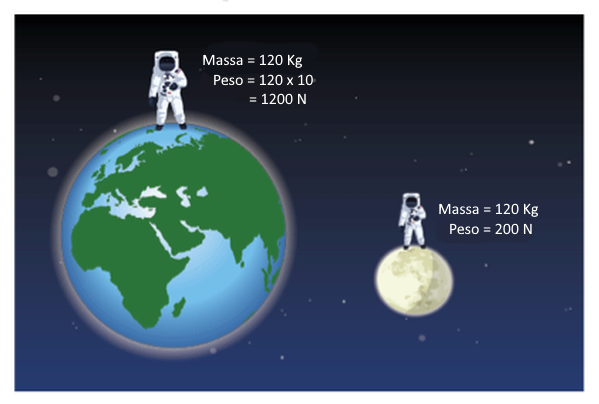
\includegraphics[width=.8\linewidth]{./image/PESTA/fisica/mass-1.png}
	\caption{Peso e Massa}
	\label{mass}
\end{figure}
Através da medição do peso, isto é, da força gravitacional exercida num dado objeto, podemos calcular a massa. \cite{book-2}
\emptyline
A massa dos objetos pode ser medida por balanças utilizando vários métodos, tais como as alavancas convencionais, ou por  molas, ou ainda sistemas mais modernos, como, as balanças digitais.
\emptyline
As balanças digitais estão presentes no nosso dia a dia e tornaram-se numa ferramenta indispensável na indústria, comércio e laboratórios. Determinar a massa dos objetos facilitou a moeda de troca no comércio, e tornou-se num pilar fundamental da física e seu desenvolvimentos.
\emptyline
Existe uma procura, tanto na área comercial como na industrial, que empurra o desenvolvimento dos sensores para obter melhores resultados, quanto à precisão e imunidade de influências exteriores na medição das grandezas mencionadas (força, torque e a massa).
\emptyline
A importância desta grandeza (massa) foi o mote para o projeto proposto: a implementação de uma balança digital para uso doméstico, recorrendo a componentes que estão disponíveis no mercado.
%%%%%%%%%%%%%%%%%%%%%%%%%%%%%%%%%%%%%%%%%%%%%%%%%%%%%%%%%%
\newpage
\section{Objetivos}
O objetivo principal deste projeto será a implementação de uma balança digital economicamente viável, usando os sensores e equipamentos disponíveis no mercado, para ter um produto útil e fácil de ser replicado.
\emptyline
Escolher o sensor adequado e meios de tratamento da informação e comunicação, será o objeto de estudo. Tendo como foco a utilização de um \textit{Embedded System} utilizando as ferramentas necessárias para o executar.
\emptyline
No final, o produto obtido será testado, de forma a tentar aperfeiçoar, fazer melhorias, alterações e adaptações que possam surgir, tendo em vista a possibilidade de simplificar o projeto e torná-lo mais atraente ao consumidor.
%%%%%%%%%%%%%%%%%%%%%%%%%%%%%%%%%%%%%%%%%%%%%%%%%%%%%%%%%%
\newpage
\section{Calendarização}
O segundo semestre teve início em 8 de Março, num ambiente de pandemia COVID-19, período durante o qual foi necessário recorrer ao ensino à distância, e todo o trabalho teve de ser acompanhado \textit{online} pelos docentes. No entanto foi necessário organizar as tarefas pretendidas de acordo com o plano abaixo descrito, para poder fazer a entrega deste trabalho antes da data limite da época normal (28 de Junho de 2021).
\begin{table}[H]
	\caption{Calendarização das tarefas}
	%\begin{sidewaysfigure}
	\begin{ganttchart}[vgrid, hgrid]{1}{20}
		\gantttitle{Março}{5} 
		\gantttitle{Abril}{5}
		\gantttitle{Maio}{5}
		\gantttitle{Juno}{5}\\
		\gantttitlelist{1,...,20}{1}\\
		%First Group
		\ganttgroup{Requisitos}{2}{10} \\
		\ganttbar{Material}{3}{5} \\
		\ganttbar{\textit{Template} LaTeX}{5}{10} \\
		\ganttbar{\textbf{IDE} \textit{Template}}{3}{10}\\
		%\ganttlink{elem0}{elem1}
		%\ganttlink{elem1}{elem2}
		%\ganttlink{elem2}{elem3}
		%\ganttmilestone{Milestone 1}{11}
		%Second Group
		\ganttgroup{Projecto}{3}{20} \\
		\ganttbar{Kit Desenvolvimento}{3}{4} \\
		\ganttbar{Montagen Mesa Sensor}{5}{7} \\%5 7
		\ganttbar{HX711 comunicação}{4}{10} \\%4 8
		\ganttbar{Programação e ensaio}{4}{20}\\
		%\ganttlink{elem4}{elem5}
		%\ganttlink{elem5}{elem6}
		%\ganttlink{elem6}{elem7}
		%\ganttmilestone{Milestone 1}{11}
		%Third Group
		\ganttgroup{Relatório}{9}{20} \\
		\ganttbar{Literatura}{8}{12} \\
		\ganttbar{Análise documentação}{9}{12} \\
		%\ganttbar{Validação}{10}{12} \\
		\ganttbar{Execução}{10}{20}
		%\ganttlink{elem8}{elem9}
		%\ganttlink{elem9}{elem10}
		%\ganttlink{elem10}{elem11}
		%\ganttmilestone{Milestone 1}{11}
	\end{ganttchart}
	\label{gantt}
%\end{sidewaysfigure}
\end{table}
%%%%%%%%%%%%%%%%%%%%%%%%%%%%%%%%%%%%%%%%%%%%%%%%%%%%%%%%%%
\newpage
\section{Organização do Relatório}
No capítulo 1 é feita uma contextualização do trabalho realizado e do seu propósito face às necessidades do mundo atual.
\emptyline
No capítulo 2 é apresentada uma breve história da evolução das balanças, e depois um estudo da balança eletrónica.
\emptyline
No capitulo 3 é apresentado a balança digital, seus componentes e características com uma descrição.
\emptyline
No capitulo 4 é descrito o software utilizado, estrutura do programa, e a implementação do código.
\emptyline
O capitulo 5 é apresentada a validação da implementação do projeto e seu funcionamento.
\emptyline
O capitulo 6 são expostas as conclusões e possíveis alterações do produto.
%%%%%%%%%%%%%%%%%%%%%%%%%%%%%%%%%%%%%%%%%%%%%%%%%%%%%%%%%%

\chapter{Evolução da balança}
%%%%%%%%%%%%%%%%%%%%%%%%%%%%%%%%%%%%%%%%%%%%%%%%%%%%%%%%%%
As balanças foram criadas por necessidade durante o desenvolvimento do comércio na antiguidade. Os produtos que não recorriam a contagem por unidades, tais como objetos irregulares (por exemplo o ouro) tinha de se quantificar o seu valor, e a forma de medir a sua massa tornou-se numa variável de medição para a troca de bens.
%%%%%%%%%%%%%%%%%%%%%%%%%%%%%%%%%%%%%%%%%%%%%%%%%%%%%%%%%%
\newpage
\section{O aparecimento e a evolução da balança}
%A relíquia mais antiga de uma balança de medir massa foi descoberta na vila de \textit{Indus River}, perto da região hoje conhecida como Paquistão, e estima-se ser por volta de 2000 A.C.
Estas primeiras balanças eram alavancas em equilíbrio. $[ \; F_{1} \times b_{1c} = F_{2} \times b_{2c} \; ]$. Nos extremos eram colocados cestos estando este conjunto centrado no seu centro de massa. Assim, se os pesos colocados nos dois cestos fossem iguais, a alavanca ficava em equilíbrio (na horizontal). Esse tipo de balança era um sistema de comparação, com recurso a pesos fixos estabelecidos como norma e designados de \textbf{contra-pesos}.
\emptyline
\begin{minipage}[!b]{0.5\linewidth}
	\begin{figure}[H]
		\flushleft
		\includegraphics[height=6cm]{./image/PESTA/general/balanca_1.jpg}
		\caption{Balança medieval}
		\label{balanca_1}
	\end{figure}
\end{minipage}
\hspace{1cm}
\begin{minipage}[!b]{0.5\linewidth}
	\begin{figure}[H]
		\centering
		\includegraphics[height=6cm]{./image/PESTA/general/balanca_4.jpg}
		\caption{Balança de laboratório}
		%\caption{Balança moderna \cite{book-7}}
		\label{balanca_4}
	\end{figure}
\end{minipage}
\minipagespace{.5}
Este sistema é prático, mas também pode facilmente ser adulterado de forma a ter leituras incorretas.
\newpage
Os métodos de medir a massa de objetos não conheceram nenhumas melhorias tecnológicas relevantes até à era industrial. Só nos fins do século \textit{XVIII} é que o meio de medir a massa de objetos não dependia de contra-pesos. As balanças por molas foram inventados por volta de 1770 em Inglaterra por \textit{Richard Salter}, um fabricante de balanças.\\
\begin{figure}[H]
	\centering
	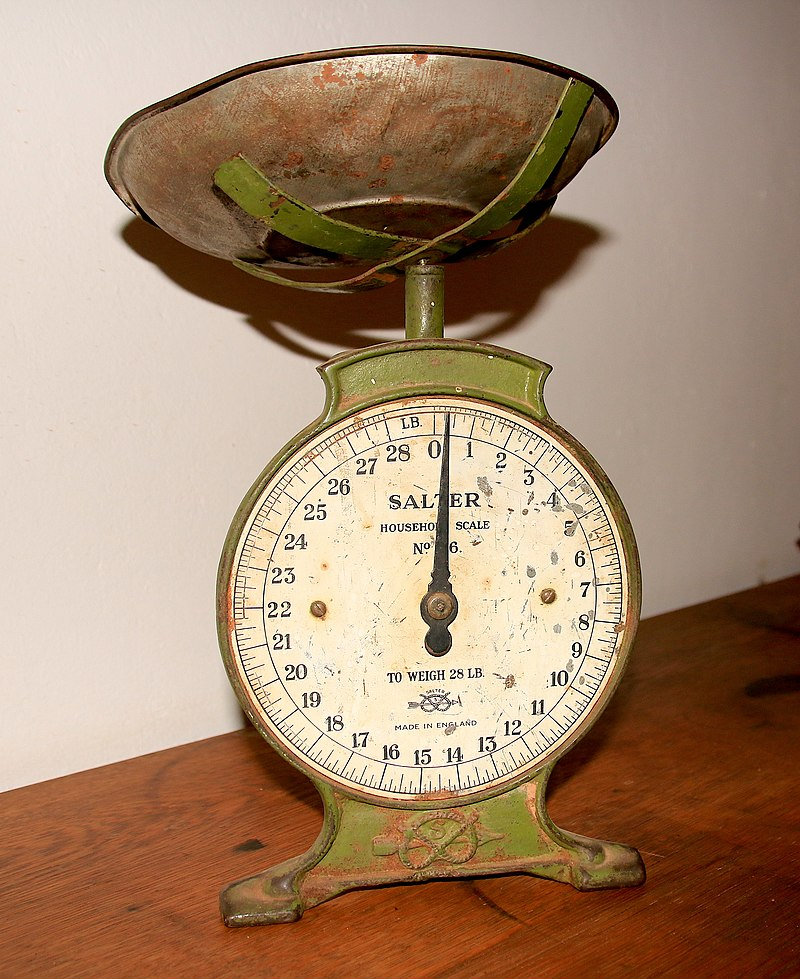
\includegraphics[scale=.15]{./image/PESTA/general/Weigh_Scale_Salter_1.jpg}
	\caption{Balança de Salter}
	\url{https://en.wikipedia.org/wiki/Salter_Housewares}
	\label{Weigh_Scale_Salter_1}
\end{figure}
\figurespace{.1}
A balança por mola, como o nome implica, mede a pressão (ou sua tensão) exercida sobre a mola para determinar a massa do objeto. Este tipo de balanças ainda é muito comum nos dias de hoje, por serem bastante económicas de fabricar, mas não têm tanta precisão como as eletrónicas desenvolvidas e aperfeiçoadas durante o século \textit{XX}.\\
\begin{minipage}[!b]{\linewidth}
	\begin{figure}[H]
		\captionsetup{justification=raggedright,singlelinecheck=false}
		\flushleft
		\hspace{.4cm}
		\includegraphics[height=6cm]{./image/PESTA/general/Public_Body_Scales_1.jpg}
		\hspace{.4cm}
		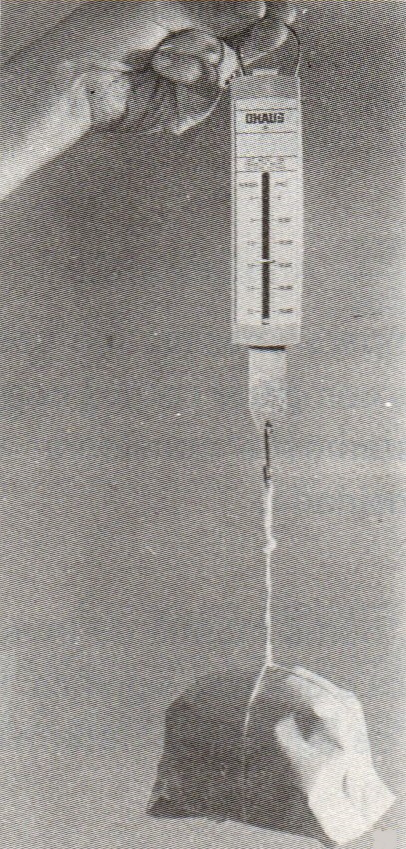
\includegraphics[height=6cm]{./image/PESTA/general/Balanca_Mola_1.jpg}
		\caption{Balanças de Mola}
		\label{Balanca_Mola_1}
	\end{figure}
\end{minipage}
%%%%%%%%%%%%%%%%%%%%%%%%%%%%%%%%%%%%%%%%%%%%%%%%%%%%%%%%%%
\newpage
\section{A balança eletrónica}
%Desenvolver mais
As balanças eletrónicas mais modernas utilizam resistências elétricas instaladas sobre materiais flexíveis por onde passa uma corrente elétrica, onde é possível detetar a variação de condutividade das resistências. Esta variação é proporcional à pressão exercida sobre esse material, trata-se dos sensores \textit{strain gauge}. As células de carga são materiais desenhados com uma estrutura para ter o mesmo comportamento de uma mola, dando-lhe uma caraterística de proporcionalidade entre a pressão exercida e o deslocamento provocado no material onde estão colocados os sensores (\textit{strain gauge}) em que detetam essa tensão mecânica e compressão. As células de carga são os sensores mais comuns usados nas balanças digitais, porque geram um sinal proporcional a força ou pressão. De notar que existem muitos tipos de células de carga para diferentes gamas de massas, porque todas as molas tem um ponto de rotura da sua elasticidade, e a partir do instante em que o mesmo é atingido, a mola perde a caraterística que a define.
\\
\begin{figure}[H]
	\centering
	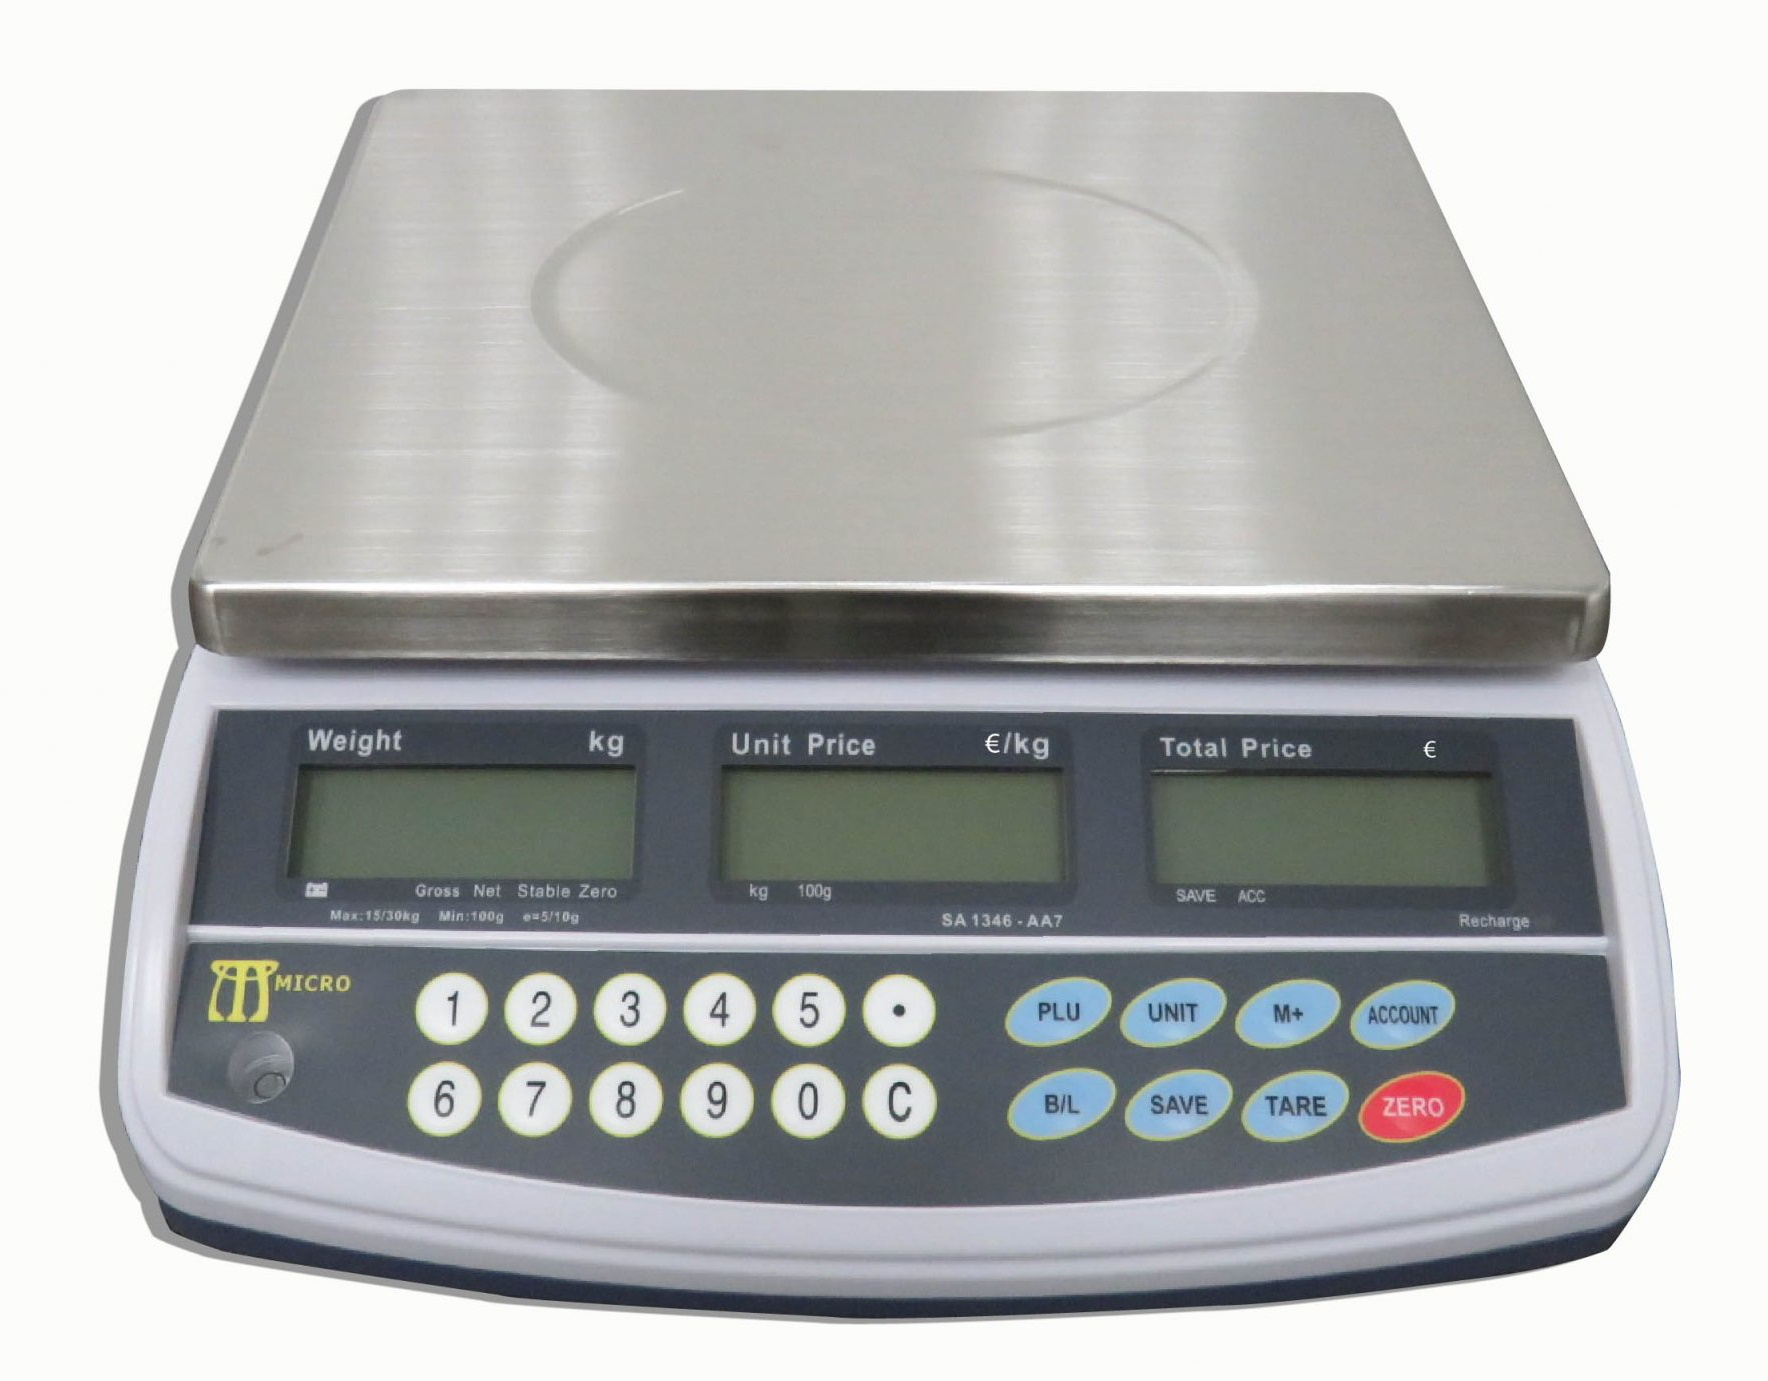
\includegraphics[height=7cm]{./image/PESTA/general/Scale_1.jpg}
	\caption{Balança eletrónica}
	\label{Scale_1}
\end{figure}
\figurespace{.5}
No projeto proposto vai ser utilizado uma \textbf{célula de carga}, que segue o princípio acima mencionado. Estas células têm sensores \textit{\textbf{strain gauges}} ligados em ponte de \textit{Wheatstone}, que vão detetar a distorção (pressão) no material da célula de carga e gerar um sinal de diferença de potencial proporcional. %Segue o mesmo princípio de uma mola.
\\
Todas as molas têm uma constante de elasticidade conhecida pela lei de Hooke \cite{book-3} \textit{equação} \eqref{eq:Hooke}.\\
%\\
%As expressões aparecem sem ligação ao texto
%Deve desenvolver mais esta parte, resultando numa mais elaborada fundamentação teórica
\begin{equation}
	\label{eq:Hooke}
	K = \frac{F}{\Delta x}
\end{equation}
\equationspace{.5}
Na \autoref{Hooke-1} temos um exemplo prático.
\begin{figure}[H]
	\centering
	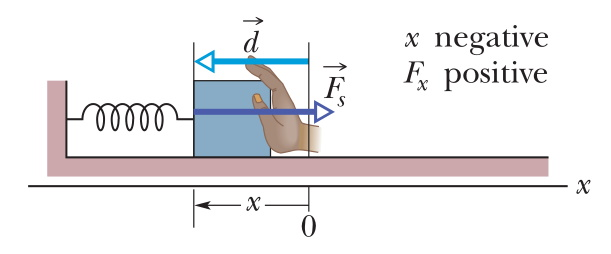
\includegraphics[height=5cm]{./image/PESTA/fisica/Hooke-1.jpg}
	\caption{Exemplo lei de Hooke \cite{book-3}}
	\label{Hooke-1}
\end{figure}
Em que.
\begin{equation}
	\label{eq:Lei-de-Hooke}
	F_x = -K \; x
\end{equation}
E a energia dissipada pela mola é determinada pela expressão \eqref{eq:Hooke-Energia}
\begin{equation}
	\label{eq:Hooke-Energia}
	W_s = - \; \frac{1}{2} \; K x^2
\end{equation}
Outros tipos de células de carga, tais como as pneumáticas e hidráulicas, convertem a pressão num sinal elétrico, que também é proporcional à força exercida, de acordo com a expressão \eqref{eq:Preasure}.
\begin{equation}
	\label{eq:Preasure}
	P = \frac{F}{A}
\end{equation}
As células de carga capacitivas são outro exemplo de como obter um sinal proporcional à força imposta como carga. Neste caso, é medida a sua capacidade, de acordo com o afastamento ou aproximação das placas dos elétrodos, de acordo com a expressão \eqref{eq:Capacity}.
\begin{equation}
	\label{eq:Capacity}
	C = \varepsilon_{0} \; \varepsilon_{r} \; \frac{A}{d}
\end{equation}
Também existem células que utilizam os princípios de ressonância, desfasamento de fase, e efeito \textit{Doppler} para determinar a pressão ou distorção, que resulta consequentemente numa medição.
%Pode-se dizer que em todos os casos se determina a força resultante através do deslocamento no espaço.
\emptyline
Como se pode observar existe diversos tipos de células de carga, é a peça principal que mede informação analógica da vida real para outra analógica de sinal elétrico, uma etapa de conversão onde podemos utilizar nos nossos sistemas eletrónicos para determinar seu valor.
\\
É nesta etapa que a seguir precisamos de outra conversão, de um sinal analógico elétrico para outro que seja do tipo discreto para poder ser tratado digitalmente, estou a falar dos \ac{adc}, e como a maioria dos sensores geram sinais com magnitude muito pequenas é frequente necessitar também de uma pré amplificação e uma filtragem de ruídos.
\\
Depois de chegar ao mundo digital, já trabalhamos com \textit{bit}, \textit{nibble} e \textit{bytes}. A partir daqui entramos num ambiente de programação, onde a informação pode ser manipulada de forma a cumprir os objetivos que se pretende, e que neste caso também vai ser objeto de estudo.
É nesta etapa que se tem de determinar que tipo de balança digital pretendemos e suas caraterísticas, pois pode-se implementar das mais simples até as mais complexas.
%%%%%%%%%%%%%%%%%%%%%%%%%%%%%%%%%%%%%%%%%%%%%%%%%%%%%%%%%%
\begin{comment}
Measurement devices need to be robust to withstand changing environmental influences such as temperature, vibration, and humidity, and they must also provide reliable measurement over long periods of time. Mechanical interfacing of the devices can be difficult and can influence final measurement. The forces and torques may change rapidly, and so the devices must have adequate frequency and transient responses.\\
There are several methods to measure forces and torques. Often, the force to be measured is converted into a change in length of a spring element. The change in dimensions is subsequently measured by a sensor, for example, a piezoresistive, a capacitive or a resonant sensor.\\
It is not so surprising, therefore, that most force and torque measurement devices utilize the long and well-established resistance strain gauge technology.\\
Unfortunately, the metallic resistance strain gauge is relatively insensitive such that in use it is normal to obtain only several millivolts of analog voltage before amplification, and the gauges must not be significantly overstrained. The rangeability and overloading capabilities are seriously restricted. Also, the gauges consume relatively high electrical power (e.g., 250 mW).\\
In general, measurement instrumentation now needs smaller sensing devices of lower power consumption and with greater rangeability and overload capabilities.\\
Greater compatibility with digital microelectronics is highly desirable. Noncontact and wireless operation is sometimes needed, and in some cases batteryless devices are desirable. Production of measurement devices using metallic resistance strain gauges can be relatively labor intensive and skilled, and may require relatively ineffi-cient calibration procedures.\\
In recent years some instrument manufacturers of force and torque measure-ment devices have moved away from using resistance strain gauges. Already, one leading manufacturer of weighing machines for retail and industrial applications now uses metallic and quartz resonant tuning fork technologies, and smaller companies have established niche markets using surface acoustic wave (SAW) technology, optical technology, and magnetoelastic technology.\\
Further commercial developments are taking place to enhance device manufacturability and improve device sensitivity and robustness in operation. Measurement on stiffer structures at much lower strain levels is now possible. The worldwide sensor research base is very active in exploring MEMS for sensing force and torque, and the rest of this chapter will review the current situation and future prospects.
\emptyline
The market pull provided by the automotive industry—for example, for manifold air pressure sensors has led to the development of successful devices and technologies that have benefited a wide range of other pressure sensing applications.
\end{comment}
%%%%%%%%%%%%%%%%%%%%%%%%%%%%%%%%%%%%%%%%%%%%%%%%%%%%%%%%%%

\chapter{Desenvolvimento do projeto}
%Neste capitulo deve fazer uma introdução na qual são indicados os requisitos do sistema a implementar. Será uma balança, mas quais as caracteristicas da mesma ? Disso depende os componentes selecionados.
Para o desenvolvimento deste projeto, foi criado um \textit{kit} de desenvolvimento o que permitiu a realização de testes, com vista à validação do projeto, bem como à execução de alterações e melhoramentos.
\emptyline
%Qual a resolução do dispaly LCD e a Gama da celula de peso.
Analisando a \autoref{Kit_Desenvolvimento_2}, pode-se verificar a montagem em esqueleto do equipamento.
\\
\begin{figure}[H]
	\centering
	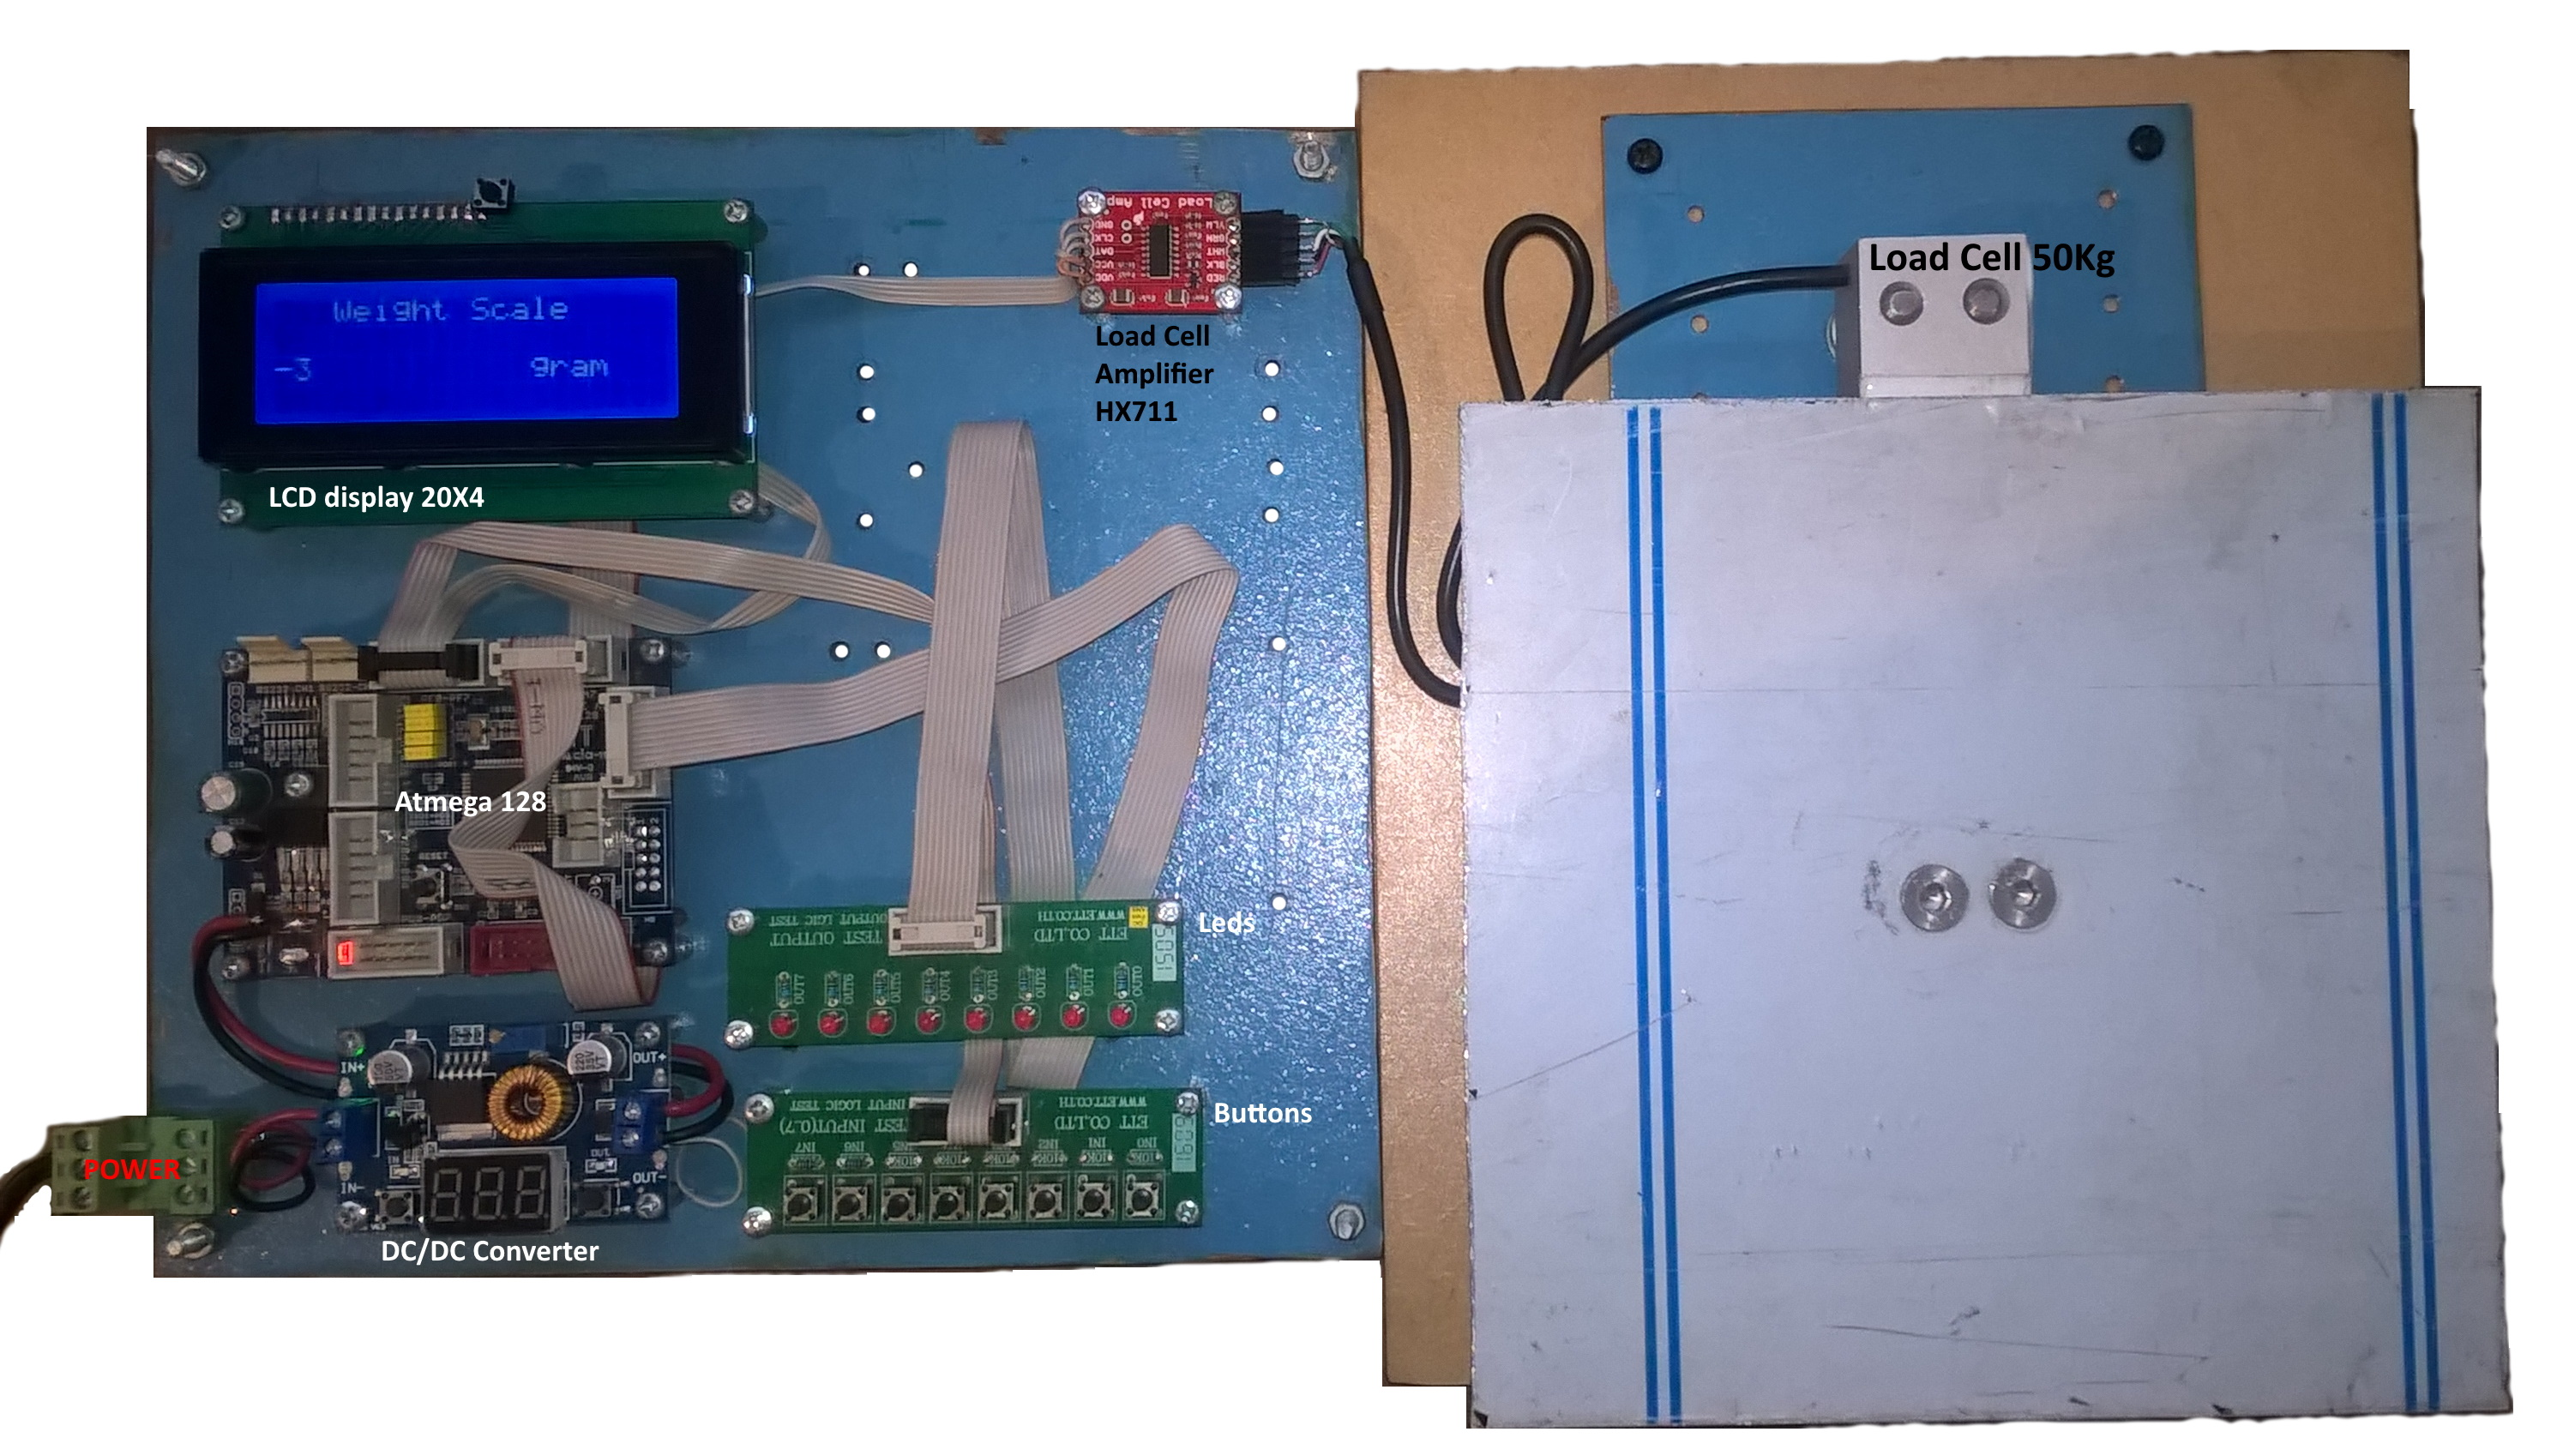
\includegraphics[scale=0.12]{./image/PESTA/kit/Kit_Desenvolvimento_2.jpg}
	\caption{Kit de Desenvolvimento}
	\label{Kit_Desenvolvimento_2}
\end{figure}
\figurespace{.5}
A seguir na \autoref{Diagrama-bloco-2} estão representados os elementos em diagrama de blocos.
\\
%Pôr a celula de caraga representada por um bloco
%comunicação série
%que tipo de comunicações ?
%O display visualiza o que ?
%O objectivo do botões e leds indicadores?
\begin{figure}[H]
	\centering
	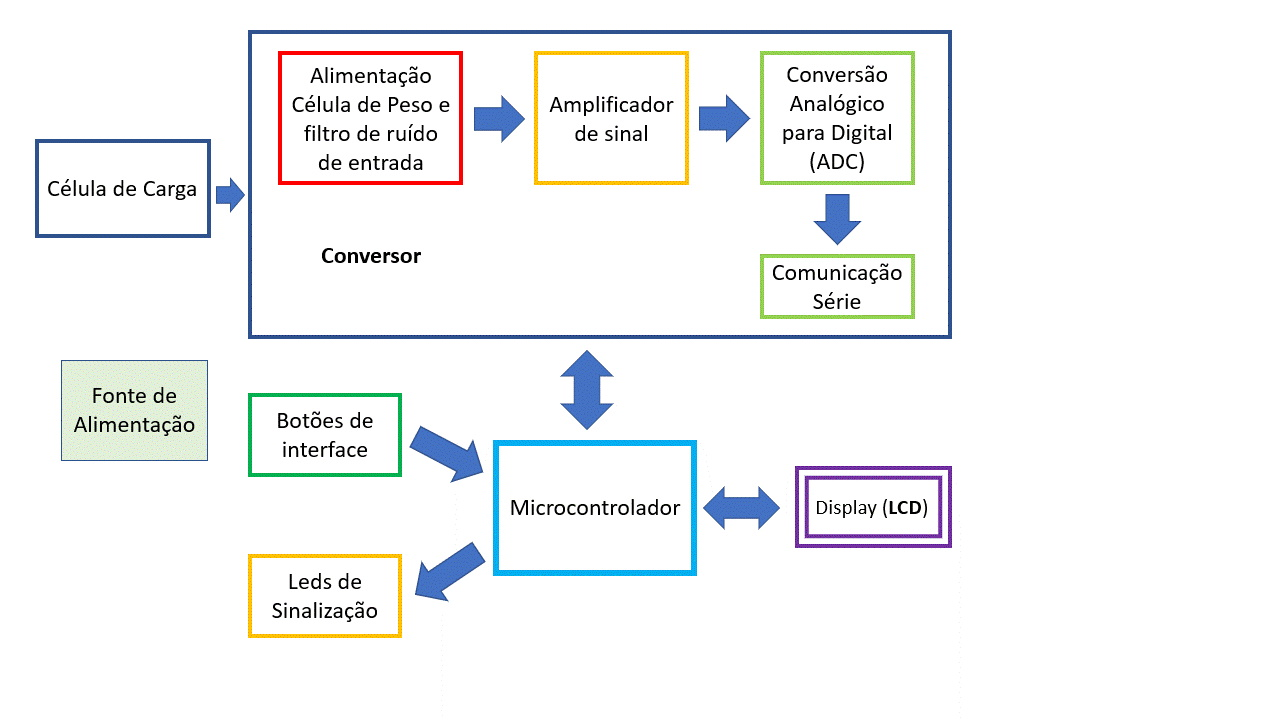
\includegraphics[scale=0.5]{./image/PESTA/Diagrama/Diagrama-bloco-2.jpg}
	\caption{Diagrama blocos do sistema implementado}
	\label{Diagrama-bloco-2}
\end{figure}
\figurespace{.5}
O microcontrolador usado neste projeto é um Atmega 128, a célula de peso é de $50 \; Kg$ com uma saída de proporção de $\; 2 \; mV/V \;$. É usado um amplificador de célula de carga com a referência HX711, que tem um protocolo de comunicação proprietário.
É utilizo um \textit{display} \acs{lcd} para visualizar os valores medidos (com a sua grandeza), e também para visualizar o fator de divisão que converte o valor lido da célula de carga pelo \acs{adc} no seu respetiva correspondente valor de massa. Os
botões são usados para saltar entre \textit{Menus} e os \acsp{led} servem como indicadores de estado, isto é, se está a usar os parâmetros \textit{default} ou de \textit{offset}.
\emptyline
Nas seguintes secções serão apresentados os componentes utilizados no projeto, assim como os aspetos relacionados com a implementação dos mesmos.
%%%%%%%%%%%%%%%%%%%%%%%%%%%%%%%%%%%%%%%%%%%%%%%%%%%%%%%%%%
\newpage
\section{Célula de carga}
Para medir a massa, recorreu-se a uma célula de carga de $50 \; Kg$ (\autoref{Load_Cell_1}). Esta célula de carga utiliza sensores piezoresistivos numa montagem em ponte \textit{Wheatstone}. Esses locais são determinados pela configuração mecânica da célula de carga de forma a obter a leitura linear e proporcional ao peso exercido, isto é, ter um comportamento similar ao de uma mola.
%explicar melhor esta parte da montagem
\\
\begin{figure}[H]
	%\captionsetup{justification=raggedright,singlelinecheck=false}
	\centering
	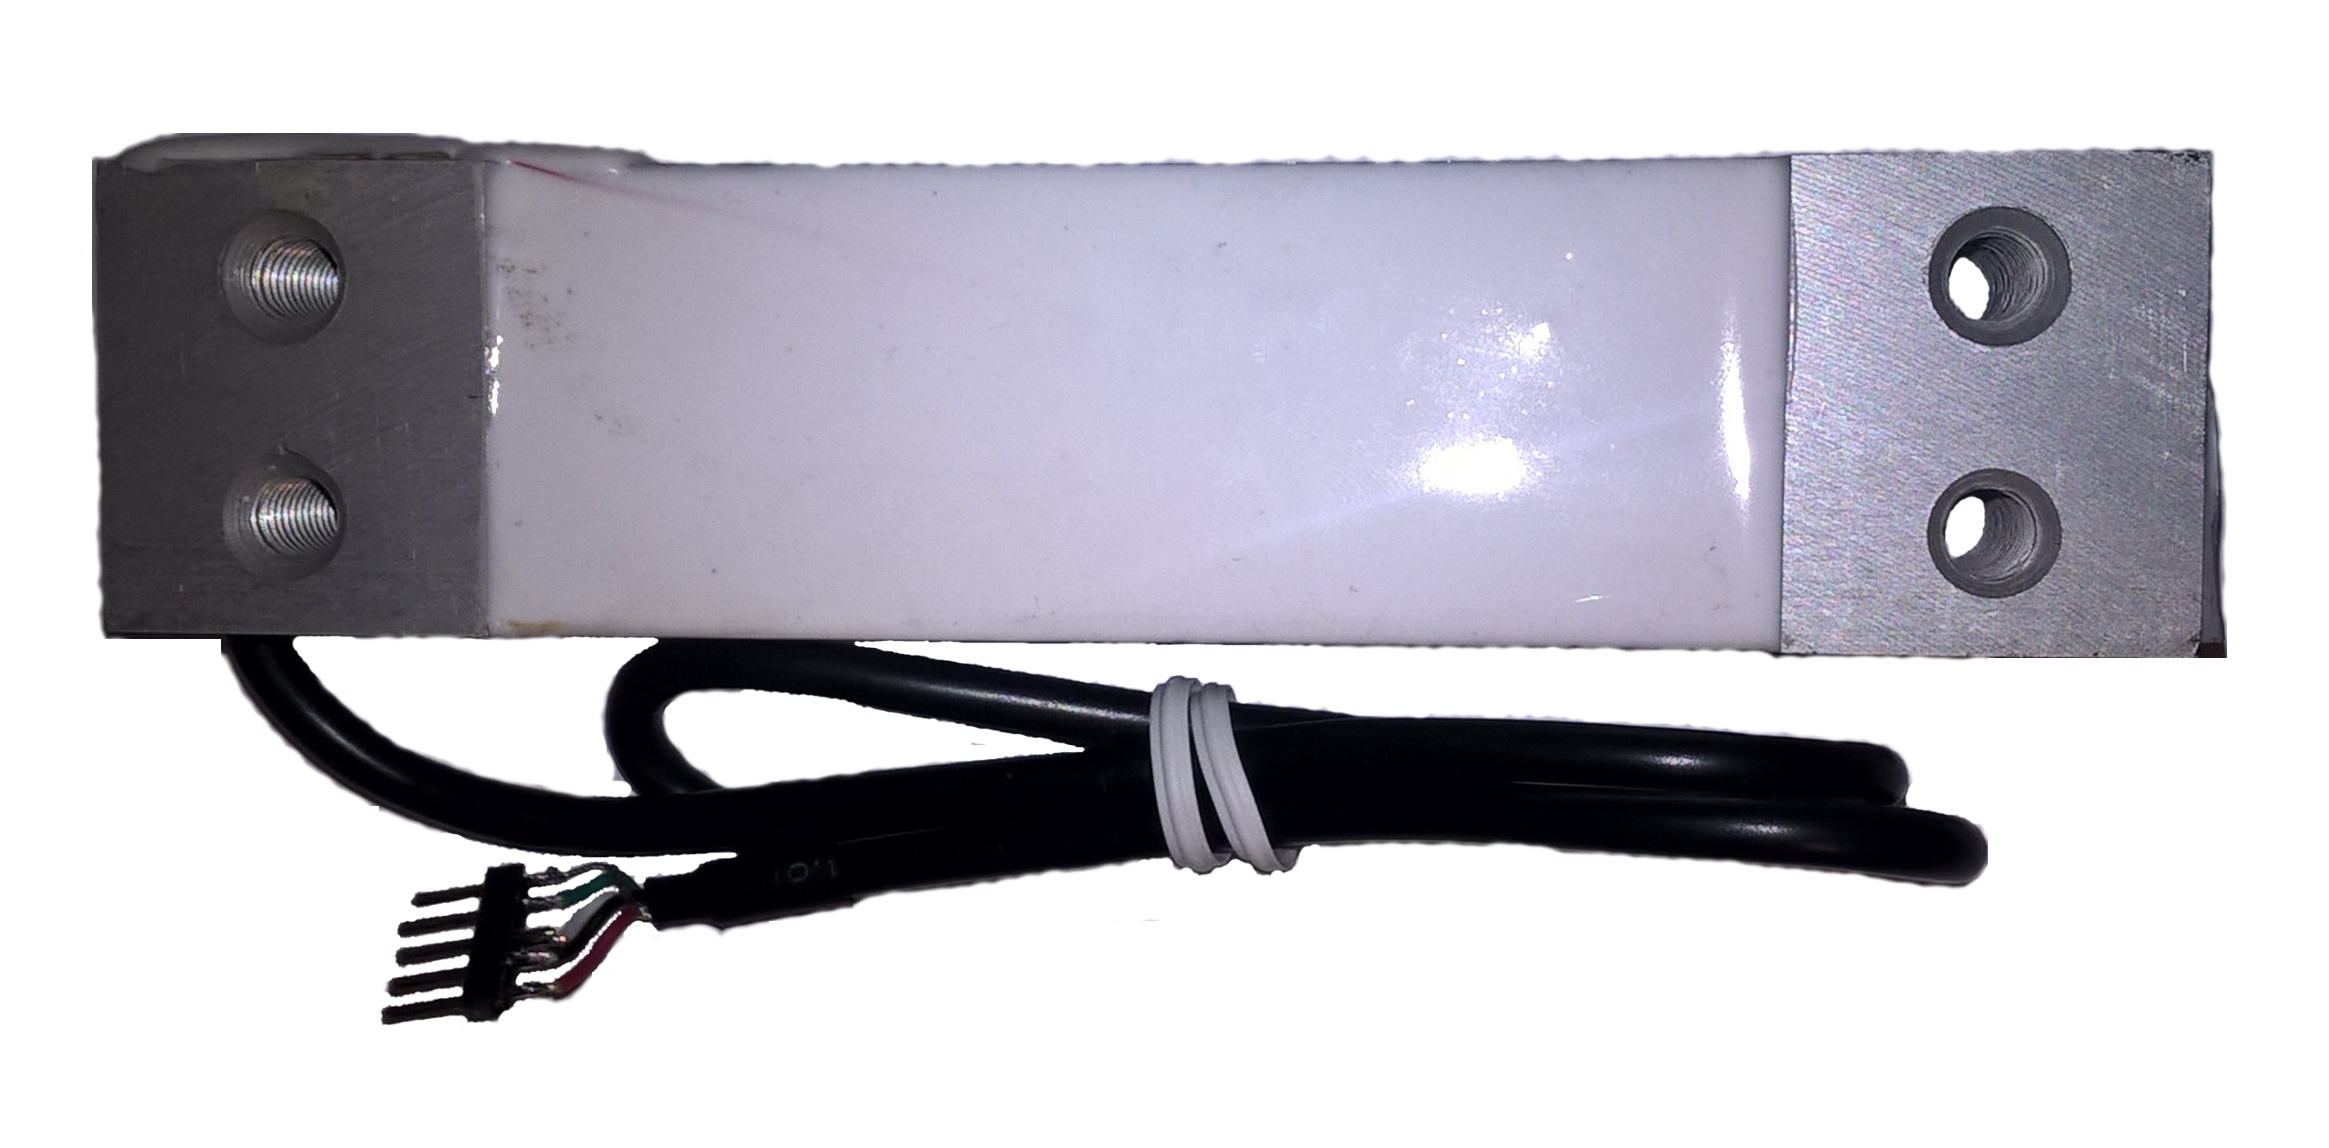
\includegraphics[scale=0.15]{./image/PESTA/material/Load_Cell_1.jpg}
	\caption{Célula de carga de $50 \; Kg$}
	\label{Load_Cell_1}
\end{figure}
\figurespace{.5}
O termo piezoresistividade deriva da palavra grega \textit{piezin}, que significa "pressionar". É um efeito exibido por vários materiais que sofrem uma mudança na resistividade devido a uma pressão aplicada. O efeito foi descoberto pela primeira vez por Lord Kelvin em 1856, que notou que a resistência dos fios de cobre e ferro aumentava quando em tensão mecânica. Ele também observou que os fios de ferro apresentavam uma alteração maior na resistência do que os de cobre. 
A primeira aplicação do efeito piezoresistivo não apareceu até à década de 1930.
\emptyline
Em vez de usar fios de metal, são geralmente feitos de uma folha de metal fina, montada numa película de suporte, que pode ser colada numa superfície. O sensor de fita de metal típico é representado na \autoref{strain_gauge_1} \cite{book-9}.
Estes sensores são implementados numa montagem do tipo ponte de \textit{Wheatstone}, de acordo com o esquema da \autoref{wheatstone-1}.
\emptyline
\begin{minipage}[!b]{.6\linewidth}
\begin{figure}[H]
	\captionsetup{justification=raggedright,singlelinecheck=false}
	\flushleft
	\figurespace{1}
	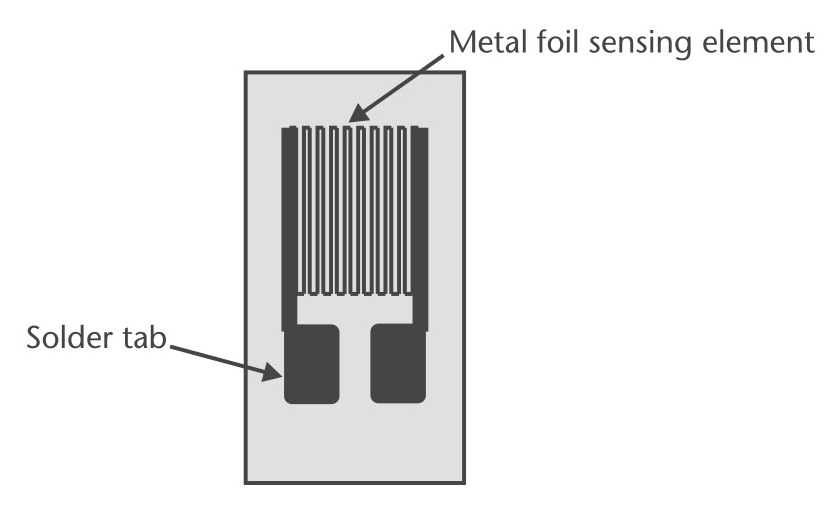
\includegraphics[height=4cm]{./image/PESTA/general/strain_gauge_1.jpg}
	\caption{Fita metálica \textit{strain gauge} \cite{book-9}}
	\label{strain_gauge_1}
\end{figure}
\end{minipage}
\begin{minipage}[!b]{.4\linewidth}
\begin{figure}[H]
	\captionsetup{justification=raggedright,singlelinecheck=false}
	\flushleft
	\vspace{1cm}
	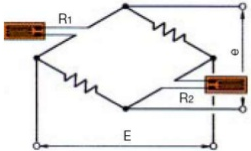
\includegraphics[height=4cm, width=4cm]{./image/PESTA/schematic/Wheatstone-1.png}
	\qquad \caption{Ponte \textit{Wheatstone}}
	\label{wheatstone-1}
\end{figure}
\end{minipage}
\minipagespace{.1}
\hspace*{1cm}\url{https://www.slideshare.net/maneeb/strain-gauge-loadcell-ppt}
%É esta a implementação utilizada no trabalho ?

%Fazer uma introdução à figura 3.6.
%Pôr sinal de massa na figura.
\vspace{.5cm}
Para uma melhor compreensão do funcionamento da ponte de \textit{Wheatstone}, a seguir é apresentado o princípio de funcionamento da ponte apenas com resistências, que está apresentada na \autoref{wheatstone-2}.
\\
\begin{minipage}[!b]{.45\linewidth}
	\begin{figure}[H]
		\captionsetup{justification=raggedright,singlelinecheck=false}
		\flushleft
		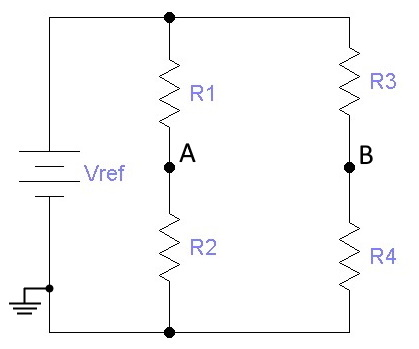
\includegraphics[height=5cm]{./image/PESTA/schematic/Wheatstone-1.jpg}
		\caption{\textit{Wheatstone} por resistências \cite{book-10}}
		\label{wheatstone-2}
	\end{figure}
\end{minipage}
\begin{minipage}[!b]{.5\linewidth}
	\setlength{\jot}{10pt}% tweak
	\small
	\begin{align}
		\label{eq:wheatstone}
		&V_A =  \frac{R_2}{R_1 + R_2} \; V_{ref} \\ &V_B=\frac{R_4}{R_3 + R_4} \; V_{ref} \\
		&V_{AB}= \left(\frac{R_2}{R_1 + R_2} - \frac{R_4}{R_3 + R_4}\right) \; Vref \\
		&V_{AB} = \frac{R_2 R_3 - R_4 R_1}{(R_1 + R_2)(R_3 + R_4)} \; Vref
	\end{align}
\vspace{1pt}
\end{minipage}
\minipagespace{.5}
É possível determinar a queda de tensão entre os pontos $A$ e $B$ do circuito ($V_{AB}$), através da diferença entre a tensão (potencial) no ponto $A$ ($V_A$) e a tensão no ponto $B$ ($V_B$).\\
Normalmente nesta configuração (\textit{Wheatstone}) só são usados um ou dois sensores como na \autoref{wheatstone-1}, e estes podem estar ligados nos extremos opostos, ou ligados ao mesmo ponto da alimentação. Só em casos muito raros são utilizados quatro sensores obtendo-se, nesse caso, uma sensibilidade máxima.
\emptyline
\emptyline
%Na \textit{figura} \ref{wheatstone-2}
Se os valores das quatro resistências são iguais, ou nos casos em que $R_2 R_3 = R_4 R_1$, então a tensão $V_{AB}$ na saída é nula, e para haver variação $V_A$ terá que ser diferente de $V_B$.\\
Analisando a \autoref{wheatstone-1}, se os valores de $R1$ e $R4$ (os sensores) variam, então existe uma variação de tensão $V_{AB}$
\emptyline
%Como demonstrado no exemplo do \autoref{wheatstone-reaction}, onde a ponte \textit{Wheatstone} tem um comportamento parabólico a uma entrada linear, em que, em certas situações é necessário uma linearização.
%\\
%\begin{minipage}[!b]{\linewidth}
%	\begin{figure}[H]
		%\captionsetup{justification=raggedright,singlelinecheck=false}
%		\centering
%		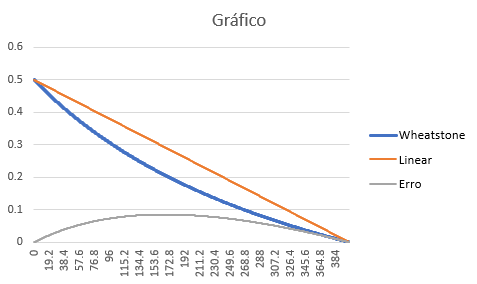
\includegraphics[height=8cm]{./image/PESTA/graph/grafico-1.png}
%		\caption{\textit{Wheatstone} comportamento}
%		\label{wheatstone-reaction}
%	\end{figure}
%\end{minipage}
%\minipagespace{.5}
Esta célula de carga de $50 \; Kg$ tem uma resolução na saída de $2 \; mV$ por cada $1 \; Volt$ da sua alimentação com mais ou menos $0.15 \; mV$ de erro. Isto quer dizer que, se for alimentada com $5 \; V$, esta vai ter na saída uma variação de tensão mínima de $10 \; mV$ e a margem de erro total de leitura está na ordem de mais ou menos $0.03\%$, segundo indicação de seu \textit{datasheet}.
Esta célula de carga tem interferências da temperatura, ruídos e se usada durante longos contínuos períodos de tempo.
\emptyline
Como indicado no \textit{datasheet} o valor obtido pode ter interferência de $0.03\%$ por cada meia hora de utilização, e $0.0016\%$ por cada grau de temperatura em excesso. Convém neste caso manter desligado o equipamento e apenas ser usado quando necessário, ou fazer \textit{offset} tendo em consideração a margem de erro.
\emptyline
%https://www.800loadcel.com/load-cell-and-strain-gauge-basics.html
%Para perceber melhor o funcionamento do sensor \textit{\textbf{strain gauge}} é aconselhável recorrer a literatura \cite{book-9} e \cite{book-10}, que explica como são feitas, seus dimensionamentos e processos de fabrico.
A montagem da mesa (prato) de medição é apresentada na \autoref{Prato}.
%Esta montagem deve ser explicada e a figura deve permitir ver todos os elementos, que devem estar devidamente identiificados
\emptyline
\begin{minipage}[!b]{\linewidth}
\begin{figure}[H]
	\centering
	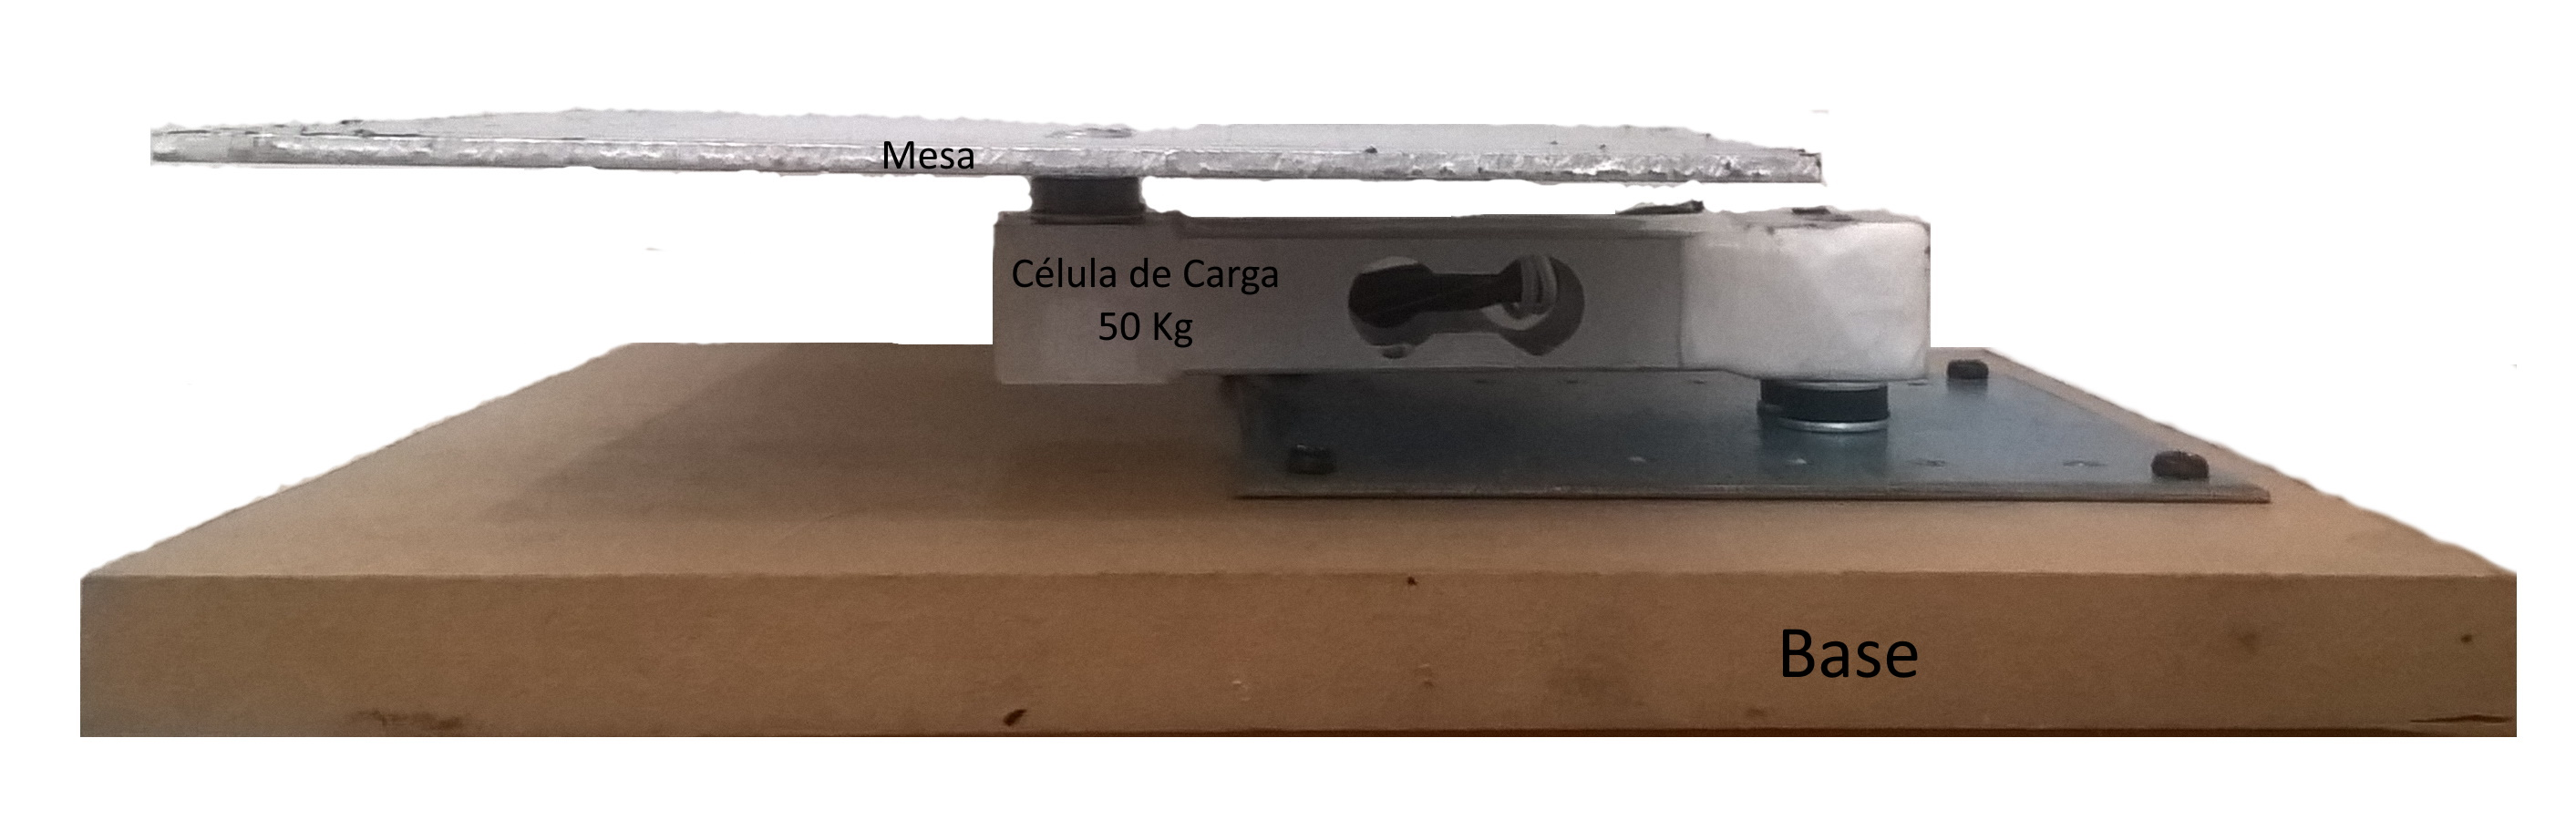
\includegraphics[scale=0.14]{./image/PESTA/material/Prato-1.jpg}
	\caption{Prato}
	\label{Prato}
\end{figure}
\end{minipage}
\minipagespace{.5}
Ao colocar uma massa sobre a mesa, esta vai exercer pressão na célula de carga, que vai resultar numa tensão mecânica e compressão nos sensores \textit{strain gauge} que estão assentes na superfície do corpo da célula de carga, provocando uma diferença de potencial correspondente. Estes sensores não estão visíveis nesta célula de carga porque esta têm uma camada protetora de silicone branco sobre eles.
%%%%%%%%%%%%%%%%%%%%%%%%%%%%%%%%%%%%%%%%%%%%%%%%%%%%%%%%%%
\newpage
\section{Amplificador de sinal e \acs{adc}}
A amplificação é geralmente um requisito fundamental, pois a maioria dos sensores tende a produzir níveis de sinal significativamente mais baixos do que aqueles usados no processador digital. Os sensores resistivos podem precisar de um amplificador para a célula de carga. Se possível, é vantajoso ter o ganho o mais próximo possível do elemento sensor, eliminado interferências de ruído e da resistência da cablagem. Em situações onde um maior ganho é necessário, muitas vezes pode haver implicações para lidar com quaisquer efeitos adversos, como o ruído, problemas de \textit{layout} do \textit{chip}, e os transitórios agudos associados aos sinais digitais que precisam de ser mantidos bem longe dos circuitos analógicos \textit{front-end}. \cite{book-9}
\emptyline
Neste projeto foi utilizado o HX711, que está apresentado na \autoref{HX711_Schematic_1}.\\
\begin{figure}[H]
	%\captionsetup{justification=raggedright,singlelinecheck=false}
	\centering
	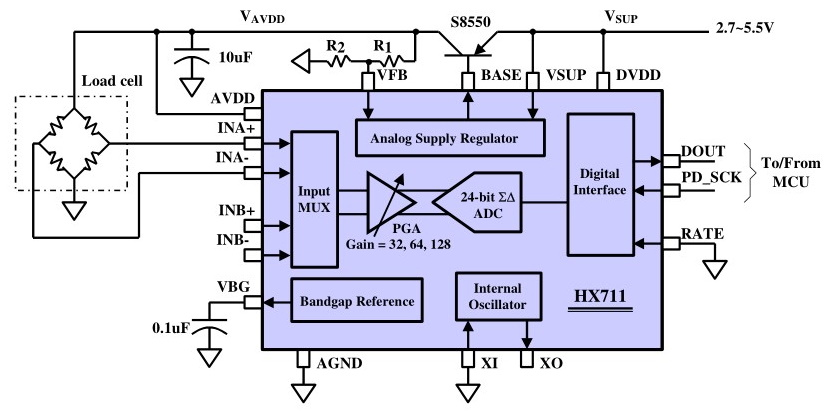
\includegraphics[scale=0.3]{./image/PESTA/schematic/HX711_Schematic_1.jpg}
	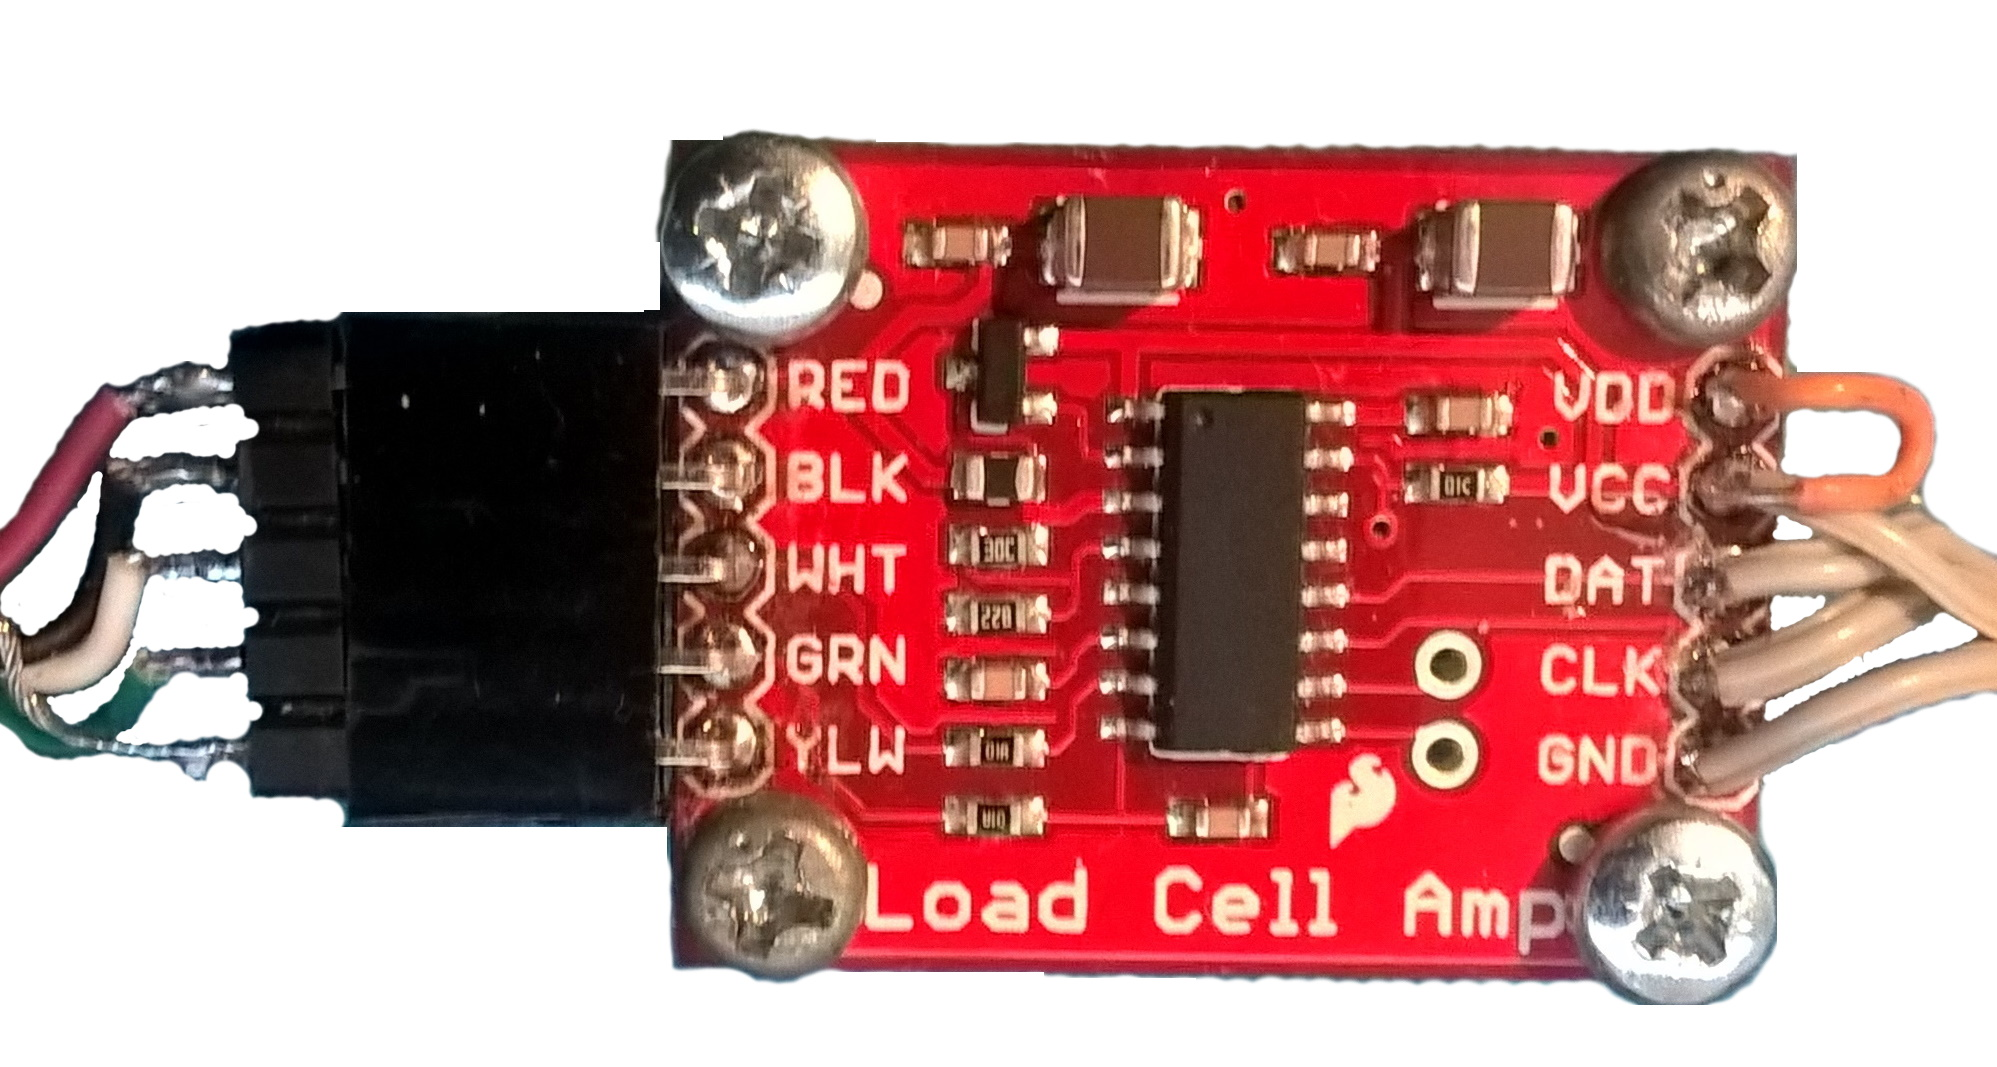
\includegraphics[scale=0.09]{./image/PESTA/material/HX711_board_1.jpg}
	\caption{Esquema de ligações e a placa do HX711}
	\label{HX711_Schematic_1}
\end{figure}
\figurespace{.5}
A ligação deste componente é fácil de se perceber tal como indicado na \autoref{HX711_connection}.\\
%Então deve ser apresentada
%Apresenatação das figuras e da tabela....
\begin{table}[H]
	\centering
	\caption{Terminais HX711 ({\tiny \scriptsize{top view}})}
	\begin{tabular}{||L{2cm} L{4cm} | p{4cm}  C{2cm}||}
		\hline
		\multicolumn{2}{||c|}{MCU} & \multicolumn{2}{|c||}{\textit{Célula de peso}}\\ [1ex]
		\hline
		1 & GND & EARTH (GND) & YLW \\ 
		2 & CLK & INPA & GRN \\
		3 & DATA & INNA & WHT \\
		4 & VCC &  GND & BLK \\
		5 & VDD & $V_{ADC}$ & RED \\ [1ex]
		\hline
	\end{tabular}	
	\label{HX711_connection}
\end{table}
\tablespace{.5}
 A parte mais complexa neste trabalho é a interligação dos equipamentos com o microcontrolador por meio de \textit{software} e a criação das bibliotecas e os \textit{drivers} de comunicação,
%como a placa do amplificador de célula de carga (\textit{chip} HX711 figura \ref{HX711_Schematic_1}),
 já que o protocolo de comunicação é proprietário. O mesmo está demonstrado na \autoref{Protocolo}.
\emptyline
Pode-se consultar a biblioteca \textit{driver} do amplificador de célula de carga HX711 nos anexos \ref{hx711-h} e \ref{hx711-c}.\\
%apresentar tabela
%A conversão AD deve ser apresentada... indicar a resolução do peso medido
\begin{figure}[H]
	%\captionsetup{justification=raggedright,singlelinecheck=false}
	\centering
	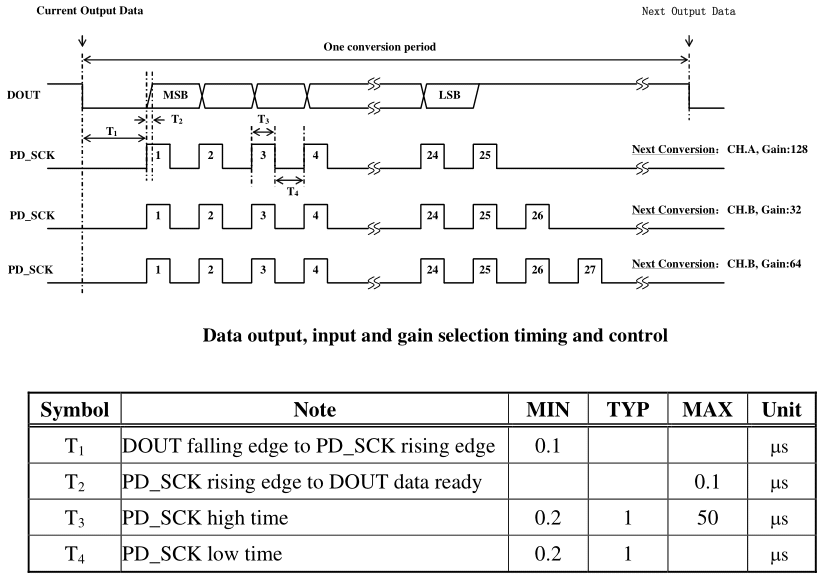
\includegraphics[scale=0.6]{./image/PESTA/comunicacao/Protocolo.png}
	\caption{Protocolo de comunicação}
	\label{Protocolo}
\end{figure}
\figurespace{.3}
A placa 
%\textit{Load Cell Amplifier}
pode ser fisicamente configurada para determinar o número de amostras por segundo a ser transmitido. Este circuito tem duas opções: a opção de 10 amostras por segundo, e de 80 amostras por segundo. Neste projeto foi utilizada a segunda opção, que necessita de uma pequena alteração na placa de circuito de impresso, isto é, é necessário abrir o respetivo \textit{jumper} de configuração.
\emptyline
A conversão de informação acontece na transição entre o sinal contínuo da vida real, para um sinal discreto associado ao mundo digital. Tipicamente esta etapa consiste na conversão de um sinal analógico para digital.\cite{book-9}\\
O processamento digital pode consistir de rotinas para compensar os desvios por linearização, a sensibilidade e o \textit{offset}, ou o processamento de técnicas mais sofisticadas como reconhecimento de padrões, (tais como, redes neuronais) para equipamentos de sensores vetoriais.\cite{book-9}\\
A comunicação é responsável por criar rotinas necessárias para transferir e receber a informação e sinais de controle, entre o sensor e o processador, que toma lugar como componente central, tratando a informação, guardando os dados e fazendo rotinas, tais como, de calibração, e de teste e controlo de ganho da amplificação. \cite{book-9}
\emptyline
Abaixo a \autoref{SPS_64} que foi adquirida do trabalho realizado recorrendo ao osciloscópio da RIGOL DS1102E e seu software \textit{Rigol Waveform Viewer}, demonstrando a comunicação entre o amplificador de sinal e o microcontrolador da informação do \acs{adc}, a linha amarela é a informação (\acs{adc}) e a azul os impulsos do \textit{clock} (PD\_SCK). Neste exemplo é visível cinco conversões executadas.\\
\begin{figure}[H]
	\centering
	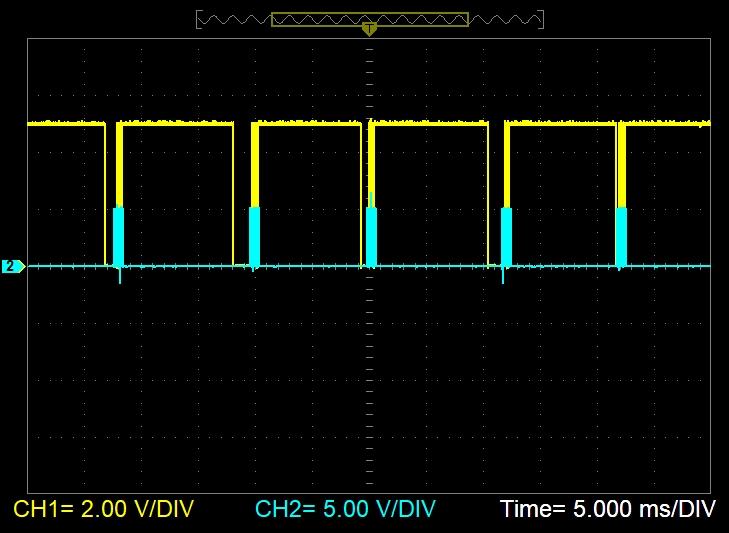
\includegraphics[scale=0.42]{./image/PESTA/graph/80SPS64GAIN/SPS_80.JPG}
	\caption{Amostras}
	\label{SPS_64}
\end{figure}
\figurespace{.1}
A biblioteca (\textit{driver}) do integrado HX711 recorre a interrupções periódicas. Quando a linha de sinal da informação (amarela) vai para a massa esta indica que tem um pacote de leitura pronto a ser transmitido.
\emptyline
\begin{minipage}[!b]{\linewidth}
\begin{minipage}[!b]{.45\linewidth}
	\begin{table}[H]
		\captionsetup{justification=raggedright,singlelinecheck=false}
		\caption{Configuração Ganho}
		\begin{tabular}{ | c | c | c |  }
			\hline
			\makecell[c]{PD\_SCK \\ Impulsos} & Entrada  & Ganho \\
			\hline
			\hline
			25 & \textbf{A} & 128 \\
			\hline
			26 & \textbf{B} & 32 \\
			\hline
			27 & \textbf{A} & 64 \\
			\hline
		\end{tabular}
		\label{Gain_Selection}
	\end{table}
	\tablespace{2.5}
\end{minipage}
\begin{minipage}[l]{.53\linewidth}
\vspace{.1cm}
Como indicado abaixo nos gráficos, em que a linha \textcolor{yellow}{amarela} é a informação e a linha \textcolor{BlueGreen}{azul} o respetivo \textit{clock} que é gerado pelas interrupções do microcontrolador, fazendo um deslocamento dos \textcolor{blue}{24} \textit{bits}, que por fim transmite para o amplificador o ganho de amplificação a ser usado pelo numero excedente de \textit{clock cycles}, em que nesta demonstração da \autoref{Gain_128_example} é \textcolor{blue}{um}, e corresponde a um ganho de \textcolor{blue}{128}, respeitando a informação apresentada na \autoref{Gain_Selection},  e de seguida o exemplo da \autoref{Gain_64_example}, com um ganho de \textcolor{blue}{64}, pois tem \textcolor{blue}{três} impulsos excedentes.
\end{minipage}
\end{minipage}
\emptyline
\begin{minipage}[!b]{\linewidth}
\begin{minipage}[!b]{.43\linewidth}
\begin{figure}[H]
	\captionsetup{justification=raggedright,singlelinecheck=false}
	\flushleft
	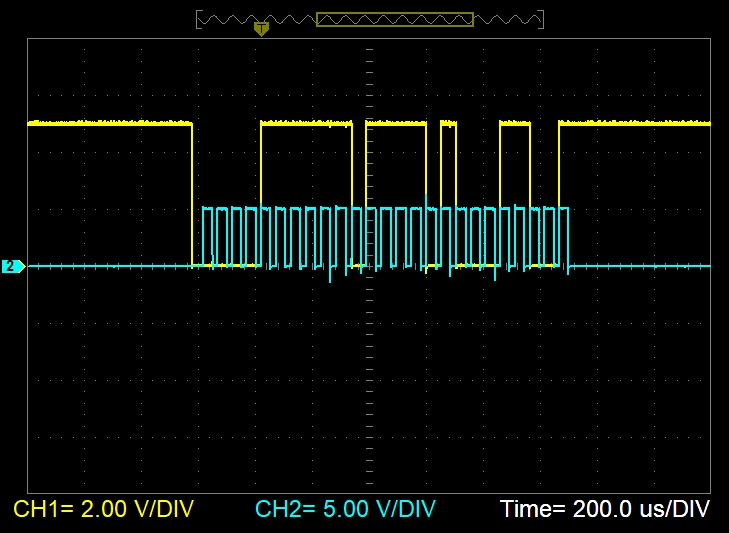
\includegraphics[scale=0.26]{./image/PESTA/graph/80SPS128GAIN/Gain_128_example.JPG}
	\caption{Ganho de 128}
	\label{Gain_128_example}
\end{figure}
\end{minipage}
\hspace{.8cm}
\begin{minipage}[!b]{.43\linewidth}
\begin{figure}[H]
	\captionsetup{justification=raggedright,singlelinecheck=false}
	\flushleft
	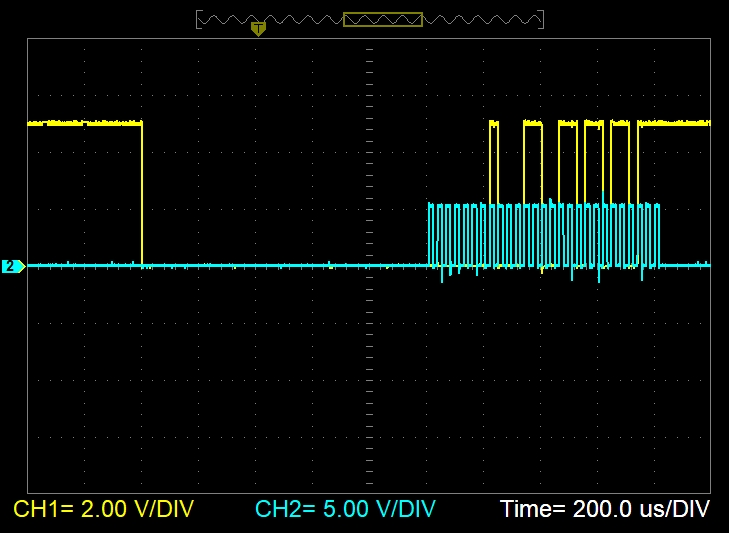
\includegraphics[scale=0.26]{./image/PESTA/graph/80SPS64GAIN/Gain_64_example.JPG}
	\caption{Ganho de 64}
	\label{Gain_64_example}
\end{figure}
\end{minipage}
\end{minipage}
\minipagespace{.5}
Para obter este resultado, a livraria \textit{driver} para o \textit{Load Cell Amplifier} teve de ter em consideração que a arquitetura do microcontrolador é de 8 \textit{bits}, uma vez que a estrutura do pacote de informação é entre 25 a 27 impulsos do \textit{clock cycle} em que é transmitido primeiro o \ac{msb}.
\emptyline
Este amplificador de célula de carga tem uma amplificação no sinal de entrada com valores indicados na \autoref{Gain_Selection}, e tem uma resolução de 24 \textit{bits}, como se sabe os números podem representar quantidades e intervalos, os 24 \textit{bits} representa um intervalo de 0 até \, $2^{24}-1$, que nos dá 16777215 unidades, ou seja, o sinal de entrada amplificado pode ser dividido por este numero, isto é, pode-se obter este número de leituras possíveis, em que, se se tratar por exemplo de 5 Volt pode-se obter 16777215 leituras de intervalos de aproximadamente $2.98 \times 10^{-7}$ Volt cada, uma precisão muito boa.
%%%%%%%%%%%%%%%%%%%%%%%%%%%%%%%%%%%%%%%%%%%%%%%%%%%%%%%%%%
\newpage
\section{Display \acs{lcd}}
%Porque este ?
%O que pretende que seja visualizado ?
O \ac{lcd} utilizado é de 4x20, isto é, quatro linhas de vinte caracteres cada, tornando-se no interface humano principal, e também durante este projeto numa ferramenta extremamente útil para fazer o \textit{debug} e executar testes ao código pela visualização das informações adversas.\\
Este \acs{lcd} é usado para visualizar as leituras e o valor de calibração da célula de carga, a escolha deste \textit{display} é unicamente por ter este componente no stock existente de material com uma biblioteca que o suporta, uso este de quatro linhas apenas para facilitar a deteção de anomalias ao testar o código visualizando vários parâmetros ao mesmo tempo.
\emptyline
%que projectos ?
%mencionar relatórios e mencionar relatorio LABSIS.
A biblioteca ou driver do \acs{lcd} que já tinha feito para outros projetos pessoais serviu para utilizar na disciplina de laboratório de sistemas \cite{article-1} e neste projeto, poupando bastante tempo, revelando a importância de documentar os conhecimentos adquiridos. A biblioteca está presente no \textit{anexado} \ref{lcd-h} e \ref{lcd-c}.
%[\ref{codigo}]
\emptyline
Abaixo está uma imagem do \acs{lcd} de 4x20 azul na \autoref{4x20_LCD} e na \autoref{LCD_connections}, suas respetivas ligações.\\
\begin{figure}[H]
	\centering
	%%\captionsetup{justification=raggedright,singlelinecheck=false}
	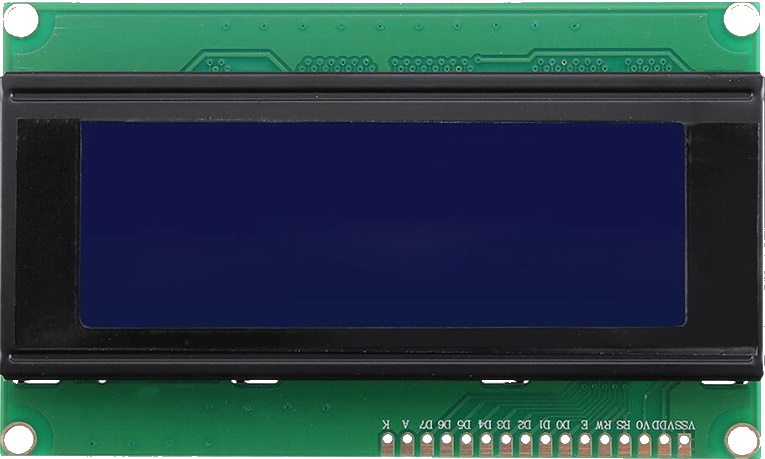
\includegraphics[height=6cm]{./image/PESTA/material/4x20_LCD.jpg}
	\caption{\acs{lcd}}
	\label{4x20_LCD}
\end{figure}
\begin{table}[H]
	\centering
	\caption{Ligações \acs{lcd}}
	\begin{tabular}{||p{1cm} p{2cm} p{4cm} | p{1cm}||} 
		\hline
		\multicolumn{3}{||c|}{\textbf{LCD Pin}} & \multicolumn{1}{|c||}{\textbf{MCU Pin}}\\ [1ex]
		\hline
		1 & VSS & GND & \\
		2 & VCC & +5V & \\
		3 & VEE & \textit{Contrast Control} & \\
		4 & RS & \textit{Register Select} & Pin 0 \\
		5 & RW & \textit{Read/Write} & Pin 1 \\
		6 & E & \textit{Enable} & Pin 2 \\
		7 & Do & \textit{Data Pin 0} & \\
		8 & D1 & \textit{Data Pin 1} & \\
		9 & D2 & \textit{Data Pin 2} & \\
		10 & D3 & \textit{Data Pin 3} & \\
		11 & D4 & \textit{Data Pin 4} & Pin 4 \\
		12 & D5 & \textit{Data Pin 5} & Pin 5 \\
		13 & D6 & \textit{Data Pin 6} & Pin 6 \\
		14 & D7 & \textit{Data Pin 7} & Pin 7 \\
		15 & LED+ & \textit{Led +5V} &  \\
		16 & LED- & \textit{Led Ground} & \\
		\multicolumn{3}{||c|}{\textit{Reboot} \acs{lcd}} & \multicolumn{1}{|l||}{Pin 3}\\ [1ex]
		\hline
	\end{tabular}
	\label{LCD_connections}
\end{table}
%%%%%%%%%%%%%%%%%%%%%%%%%%%%%%%%%%%%%%%%%%%%%%%%%%%%%%%%%%
\newpage
\section{Microcontrolador}
Os microcontroladores da Atmel de 8 a 32 \textit{bits} são baseados na arquitetura avançada de Harvard, na qual está concebido para baixo consumo e alta performance.
\emptyline
Este tipo de arquitetura tem dois \textit{buses} (barramentos), um dedicado à leitura das instruções a executar e outro para a escrita e leitura de dados (informação ou dados), isto assegura que uma nova instrução pode ser executada em cada ciclo de relógio, em que elimina todos os estados de espera, quando não há instruções prontas a executar.
\emptyline
Nos microcontroladores do \ac{avr}, os barramentos estão configurados de forma a dar prioridade ao barramento das instruções do \ac{cpu} acesso à memória flash, enquanto o barramento da \acs{cpu} de dados tem prioridade de acesso à \ac{sram}.
\emptyline
O espaço de memória de dados é dividido em três partes, os \ac{gpr} as \ac{sfr} ou memória de I/O e a \textit{data} \acs{sram}.
\emptyline
Os microcontroladores da \acs{avr} utilizam uma arquitetura de instruções \ac{risc} que reduz a complexidade dos circuitos na codificação de cada instrução. Daí que os microcontroladores que se baseiam nestes tipos de arquitetura são sinónimo de código reduzido, alta performance e baixo consumo energético.\\
\begin{figure}[H]
	\centering
	%%\captionsetup{justification=raggedright,singlelinecheck=false}
	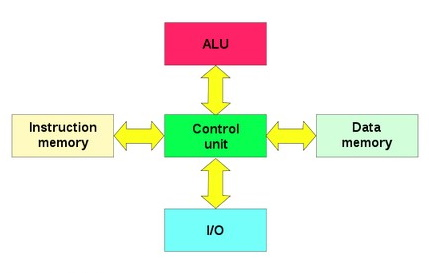
\includegraphics[scale=.75]{./image/PESTA/Diagrama/Harvard_architecture.jpg}
	\caption{Harvard Architecture}
	\label{Harvard_architecture}
	\vspace{.1cm}
	\qquad link: \url{https://en.wikipedia.org/wiki/Harvard_architecture}
\end{figure}
\figurespace{.1}
%\qquad link: \url{https://en.wikipedia.org/wiki/Harvard_architecture}
%Porque esta opção?
%O facto de ser um dos masi poderosos.. não é justificação
%A seleção do material deve ser justificada de forma mais citeriosa
%Devia ser feita uma pesquisa de produtos e seleção baseada nos requisitos prédefinidos.
O Atmega 128 (\autoref{Atmega_128_pinagem}) é um dos mais poderosos \ac{mcu} da linha de 8 \textit{bits} da Atmel, e neste projeto esta integrado numa placa de desenvolvimento dotado de ligações por fichas \ac{idc}, ou seja, utiliza \textit{flat ribbon cables} para ligar os periféricos, o que é muito mais prático do que sistemas que atualmente são mais populares, como por exemplo a placa de desenvolvimento Arduino, STMicroelectronics e a \ac{pic} que recorrem a um interface por pinos (\textit{pin headers}).\\
\begin{figure}[H]
	\centering
	%%\captionsetup{justification=raggedright,singlelinecheck=false}
	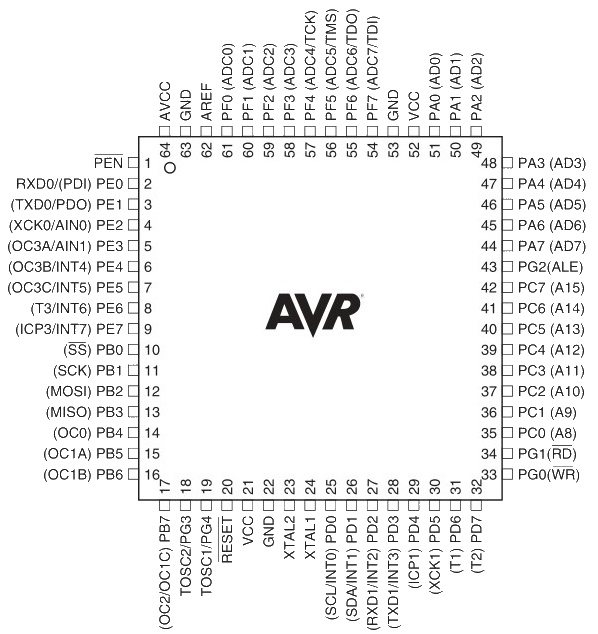
\includegraphics[scale=0.5]{./image/PESTA/material/Atmega128_1.jpg}
	\caption{Atmega 128}
	\label{Atmega_128_pinagem}
\end{figure}
\figurespace{.5}
%{Transparências Sistemas Digitais 2 \quad \acs{isep} \quad 2008/2009 \quad \textit{link}}: \\
%\url{https://drive.google.com/file/d/1wgOGf8WwYY0OzDhRca9ypXz-iBO55YOF/view?usp=sharing} \\ \\
Esta opção preenche os requisitos requeridos, por ter portas de entrada e saída suficientes, porque o \acs{lcd} requer a utilização de oito pinos para funcionar, o amplificador de célula de carga dois pinos, temos quatro botões que requer quatro pinos de entrada e três \textit{leds} indicadores, ou seja, três pinos de saída. Por aqui deduzimos que o \acs{mcu} a escolher tem que ter mais do que dezasseis pinos só para os periféricos.\\
O \acs{mcu} também tem que ter dois temporizadores capazes de gerar os tempos desejados por interrupções, talvez seria possível fazer isto com um micro controlador com menos capacidades, porque este projeto não utiliza a funcionalidade do \acs{adc} nem comunicações série integradas, no entanto comparando a nível de preço com as alternativas destaca-se esta opção.
\newpage
Alternativas que foram postas em consideração estão na \autoref{Boards-1}, e foram excluídas pelos motivos mencionados.\\
\begin{figure}[H]
	\centering
	%%\captionsetup{justification=raggedright,singlelinecheck=false}
	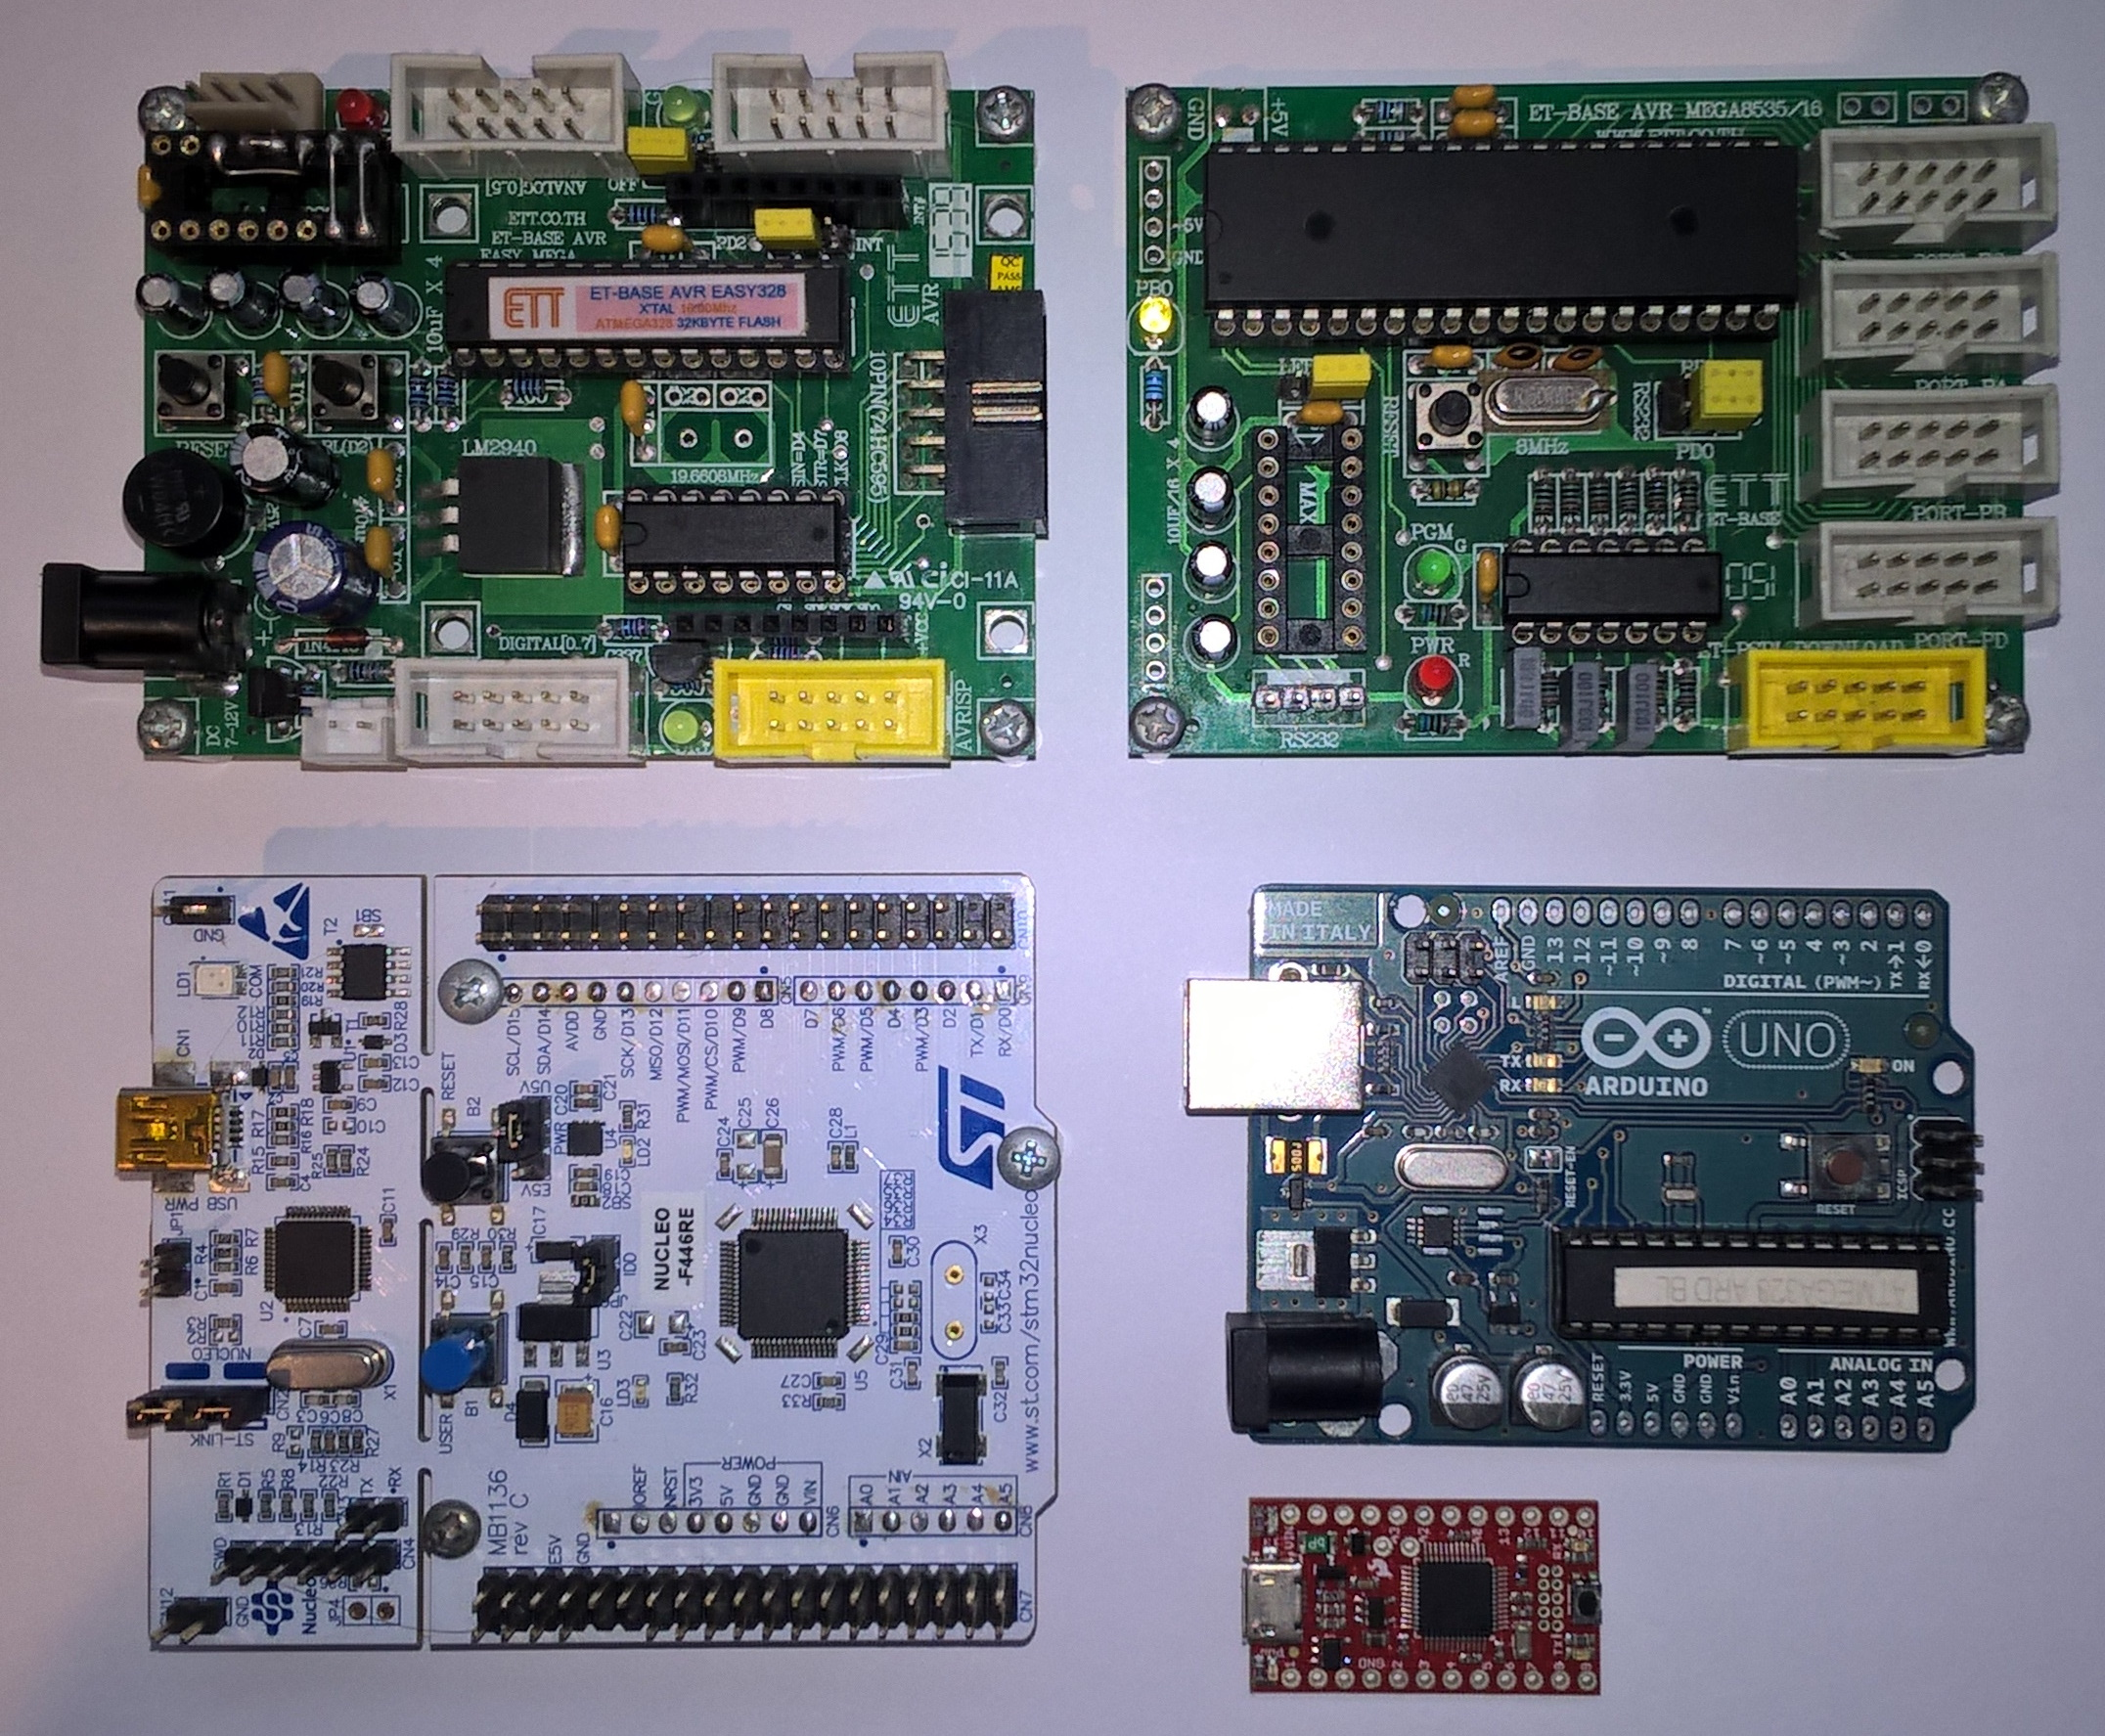
\includegraphics[scale=0.15]{./image/PESTA/boards/Boards-2.jpg}
	\caption{Alternativas ao Atmega 128}
	\label{Boards-1}
\end{figure}
\figurespace{.2}
Dos componentes que constituem o Atmega 128, os temporizadores são os que considero os mais importantes devido a ser uma das grandezas fundamentais, o tempo, podendo este gerar intervalos de tempo e \acp{pwm}
%porque
, o \ac{adc} do \acs{mcu} nem vai ser usado neste projeto, vai ser utilizado um \textit{load cell amplifier} externo, uma alternativa que é muito melhor porque tem maior resolução e específico para a aplicação em causa.
\emptyline
Talvez os \acsp{mcu} nem deviam ter a componente \acs{adc} e realçar em meios de comunicação e memoria, tornava-se assim num sistema unicamente digital.
O Atmega 128 é uma escolha acertada para este projeto, considerando as alternativas de optar por um \ac{mcu} de 32 \textit{bits} ou um \textit{embedded system} com sistema operativo integrado, em que no primeiro caso o grau de dificuldade é acrescida devido a ter muito mais configurações e funcionalidades, e a segunda opção de ser exagerada, devido a só utilizar uma muito pequena parte das suas possibilidades, como se diz em inglês um \textit{overkill}, desperdiçando recursos desnecessariamente, e também se iria refletir a nível de custos monetários, no entanto facilita bastante no desenvolvimento de qualquer projeto, pois estaria-se a trabalhar sobre uma camada de nível superior (\textit{Kernel}).
\emptyline
\begin{minipage}{\linewidth}
%{\Large Características do Atmega 128 :}
As características do microcontrolador Atmega 128 :
\normalsize
\begin{itemize}	
	\setlength\itemsep{-0.3em}
	\item Arquitectura \acs{risc}
	\item 33 instruções (a maior parte executada num único ciclo de execução)
	\item 32 x 8 registos de trabalho (arquitectura de registos)
	\item Até 16 \acs{mips} (@16MHz) – 62.5ns / instrução
	\item 64K x 16 palavras de programa – 128K bytes FLASH
	\item 4K bytes de \acs{ram} interna
	\item 4K bytes de E2PROM de dados
	\item Ciclos de escrita / leitura – FLASH=10000, E2PROM=100000
	\item 7 Portos de IO \\
		\hspace*{.5cm}	-> 6 x 8 bits (Portos A .. F) \\
		\hspace*{.5cm}	-> 1 x 5 bits (Porto G)
	\item 2 x Timer / Counter de 8 bits
	\item 2 x Timer / Counter de 16 bits
	\item 1 x Real Time Counter ( com oscilador independente)
	\item 2 x \acs{pwm} de 8 bits
	\item 6 x \acs{pwm} de 16 bits
	\item \acs{adc} de 10 bits (8 canais)
	\item 2 x \acs{usart}
	\item \acs{spi}
	\item \acs{twi} (I2C)
\end{itemize}
\end{minipage}
\minipagespace{.2}
Para programar este microcontrolador (\textbf{Atmega 128}), foi utilizado o programador da marca da Atmel, o \ac{atmel-ice} \autoref{Programador_1}. Para este equipamento tem disponível programação via \ac{isp} \autoref{ISP_6_8_10pin} e \ac{jtag}.\\
\begin{minipage}[!b]{.5\linewidth}
	\begin{figure}[H]
		\captionsetup{justification=raggedright,singlelinecheck=false}
		\flushleft
		\includegraphics[scale=0.65]{./image/PESTA/programador/Atmel_ice.png}
		\caption{KIT \acs{atmel-ice}}
		\label{Programador_1}
	\end{figure}
\end{minipage}
\hspace{.5cm}
\begin{minipage}[!b]{.5\linewidth}
	\begin{figure}[H]
		\captionsetup{justification=raggedright,singlelinecheck=false}
		\flushleft
		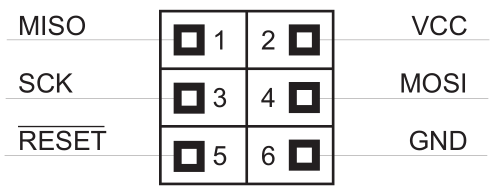
\includegraphics[scale=0.35]{./image/PESTA/programador/isp_6pin.png}
		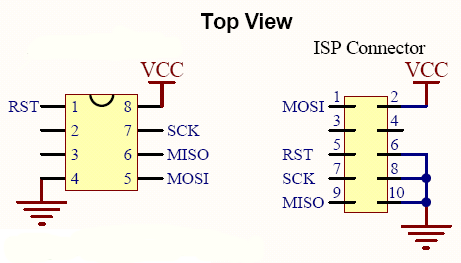
\includegraphics[scale=0.5]{./image/PESTA/programador/isp_8e10pin.png}
		\caption{Fichas \acs{isp}}
		\label{ISP_6_8_10pin}
	\end{figure}
\end{minipage}
%%%%%%%%%%%%%%%%%%%%%%%%%%%%%%%%%%%%%%%%%%%%%%%%%%%%%%%%%%
\newpage
\section{Fonte de Alimentação}
%Introdução a fonte de alimentação...
Está se a usar uma fonte de alimentação comutada abaixadora \autoref{buck-converter}, ou seja, a tensão na sua saída é sempre inferior a da sua entrada e tem uma eficiência até $96\%$.\\
\begin{minipage}[!b]{.5\linewidth}
	\begin{figure}[H]
		\captionsetup{justification=raggedright,singlelinecheck=false}
		\flushleft
		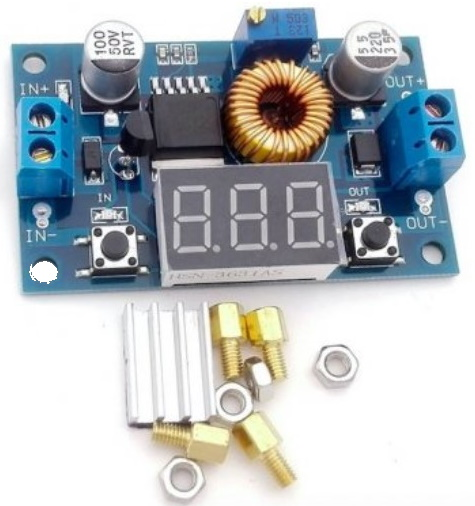
\includegraphics[scale=0.5]{./image/PESTA/material/DCDC_converter.jpg}
		\caption{\textit{Buck Converter}}
		\label{buck-converter}
	\end{figure}
	\figurespace{.1}
\end{minipage}
\begin{minipage}[!b]{.5\linewidth}
\small
Características DC/DC:
	\begin{itemize}
		\setlength\itemsep{-0.5em}
		\footnotesize
		\item 5A 75W Conversor Abaixador (\textit{Step-down})
		\item Alimentação Entrada: 4 - 38VDC
		\item Tensão de saída: 1.25 - 36VDC
		\item Corrente saída: 0 - 5A
		\item Potência saída: 75W
		\item Voltímetro: 4 até 40V, erro ±0.1V
		\item \textit{Led} indicadores
		\item Frequência de operação: 180KHz
		\item Eficiência até 96 \%
		\item Proteção Térmica
		\item Limitador de Corrente
		\item Proteção contra curto circuito
		\item NOTA: Não tem proteção de inversão de polaridade
		\item L x W x H = 6.6 x 3.9 x 1.8 CM
		\item Massa: 28g
	\end{itemize}
\end{minipage}
\minipagespace{.5}
Como a \textit{mainboard} tem um regulador de tensão linear de $5 \; Volt$, para aumentar a eficiência e ter uma alimentação variável de entrada até $38 \; VDC$ foi utilizado o \textit{buck converter} para alimentar o regulador de tensão linear para um valor próximo dos $5 \; Volt$, por exemplo $9 \; Volt$, porque se sabe que as perdas de um regulador de tensão linear é proporcional a queda de tensão entre a sua entrada e a sua saída. Podia-se remover o regulador de tensão linear e apenas utilizar o \textit{buck converter} regulado para o valor de $5 \; Volt$ mas pretende-se não alterar o \acs{pcb} da \textit{mainboard}.
%Explicar melhor
%%%%%%%%%%%%%%%%%%%%%%%%%%%%%%%%%%%%%%%%%%%%%%%%%%%%%%%%%%
\newpage
\section{Orçamento do material}
Abaixo na \autoref{Material-1}, é apresentado a lista do material utilizado no projeto, bem como o seu preço.\\
%O orçamento deve estar num anexo, ou no capítulo da apresentação dos componentes, não na validação
\begin{table}[H]{
		\caption{Lista de material}
		\rowcolors{3}{blue!80!yellow!50}{blue!70!yellow!40}
		\begin{tabular}{ |p{9cm}|c|p{2cm}|  }
			\hline
			\multicolumn{3}{|c|}{Lista de Material} \\
			\hline
			Peça & Quant & Preço [uni] \\
			\hline
			Fonte de alimetação 12V 1A & 1 & \EUR{3.87} \\
			Conversor DC-DC com voltímetro & 1 & \EUR{7.75} \\
			ET BASE AVR Atmega128 Board & 1 & \EUR{23.92} \\
			Test Input Board  & 1 & \EUR{3.71} \\
			Test Output Board & 1 & \EUR{3.71} \\
			\acs{idc} Socket 10 way    & 12 & \EUR{0.31} \\
			\acs{idc} Header Straight 10 way    & 12 & \EUR{0.25} \\
			Flatcable    & ? & \EUR{?} \\
			20x4 \acs{lcd} Module Blue & 1 & \EUR{12.24} \\
			SparkFun Load Cell Amplifier HX711 & 1 & \EUR{13.04}   \\
			50Kg Load Cell & 1 & \EUR{12} \\
			\hline
			& \textit{total} & \EUR{86.96} \\
			\hline
		\end{tabular}
		\label{Material-1}
	}
\end{table}
\tablespace{.5}
Os preços são o que estão disponíveis no mercado. Quanto a \textit{mainboard}, o preço do \acs{mcu} Atmega 128 foi o mais competitivo. Outras alternativas, de \acs{mcu} de igual ou menor capacidade, atingiam o mesmo preço ou até seriam mais caras.
%%%%%%%%%%%%%%%%%%%%%%%%%%%%%%%%%%%%%%%%%%%%%%%%%%%%%%%%%%

\chapter{Software}
%%%%%%%%%%%%%%%%%%%%%%%%%%%%%%%%%%%%%%%%%%%%%%%%%%%%%%%%%%
Neste capitulo são apresentadas as ferramentas usadas no desenvolvimento do programa, e a estrutura do mesmo. Serão ainda apresentadas algumas explicações acerca do modo como o código foi implementado de forma ser atingido o objetivo proposto, que é o correto funcionamento da balança digital.
%%%%%%%%%%%%%%%%%%%%%%%%%%%%%%%%%%%%%%%%%%%%%%%%%%%%%%%%%%
\newpage
\section{Software}
O \ac{ide} utilizado neste trabalho foi o \textbf{\textit{{Microchip Studio for AVR\textsuperscript{\textregistered} and SAM Devices}}} (\textit{version: 7.0.2542}).
\emptyline
\begin{minipage}[!b]{.55\linewidth}
	\begin{figure}[H]
		\captionsetup{justification=raggedright,singlelinecheck=false}
		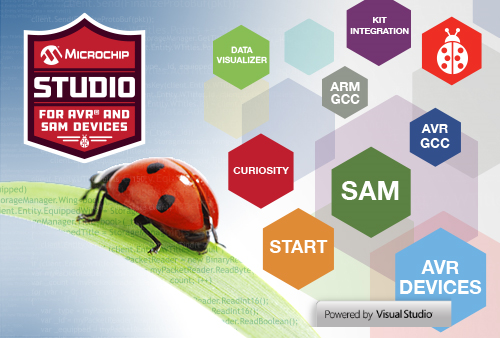
\includegraphics[scale=0.55]{./image/PESTA/IDE/Microchip-Studio.png}
		\caption{Microchip Studio}
		\label{Microchip-Studio}
	\end{figure}
\end{minipage}
\begin{minipage}[!b]{.45\linewidth}
	Ao lado a \autoref{Microchip-Studio} mostra o logo da empresa, e abaixo a \autoref{Work-Space} apresenta o ambiente de trabalho onde é criado todo o código que vai correr no microcontrolador.
\emptyline
\end{minipage}
\minipagespace{.5}
\begin{figure}[H]
	\centering
	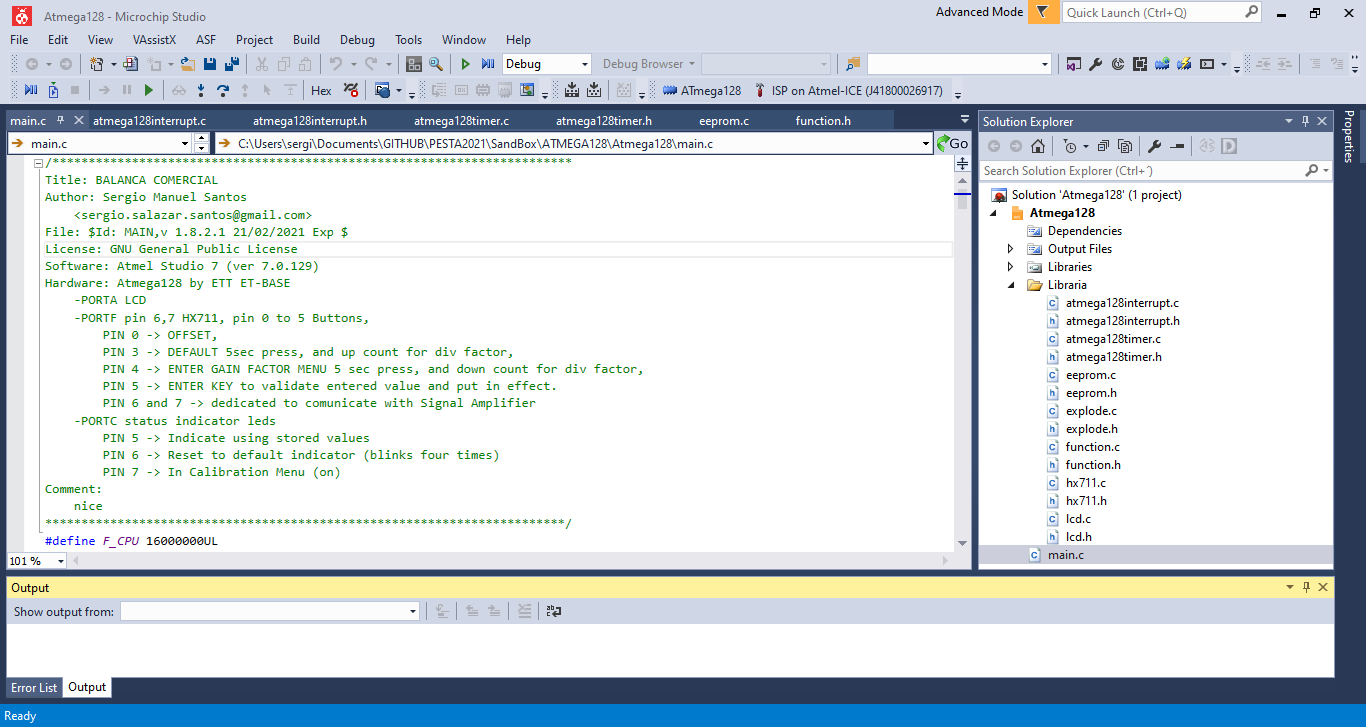
\includegraphics[width=\linewidth]{./image/PESTA/IDE/Work-Space.png}
	\caption{Ambiente de trabalho}
	\label{Work-Space}
\end{figure}
\figurespace{.5}
A programação foi feita em Linguagem \textbf{C} \cite{book-11}, e a sua estrutura sintática está abaixo apresentada na \autoref{Main_Program_1}:
\emptyline
%Mudar para Português
\begin{figure}[H]
	\centering
	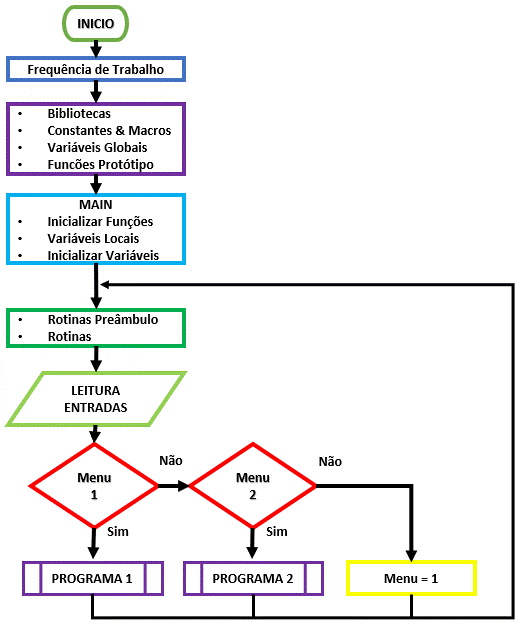
\includegraphics[scale=1]{./image/PESTA/flowchart/Main-Program-1.jpg}
	\caption{Estrutura do Programa}
	\label{Main_Program_1}
\end{figure}
\figurespace{.5}
O \textit{PROGRAMA 1} é onde corre o programa da balança, e o \textit{PROGRAMA 2} é usado para a calibração do fator de ganho.
\newpage
%O modelo de programação segue uma estrutura sintática de acordo com o seguinte modelo.
%\\
%\begin{figure}[H]
%	\centering
%	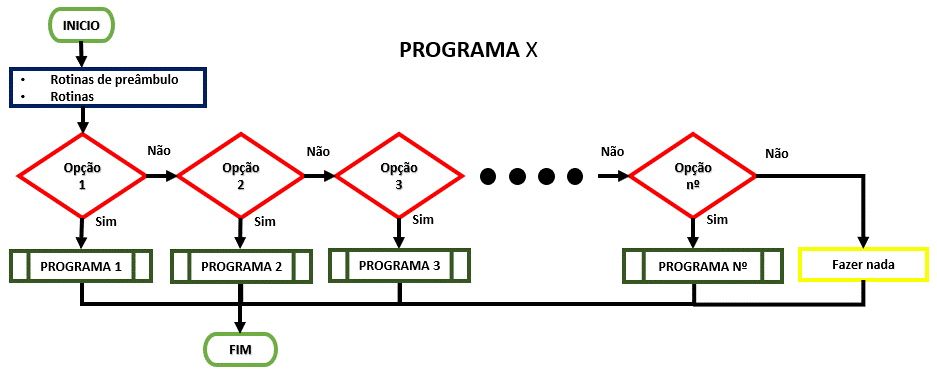
\includegraphics[height=8cm, width=\linewidth]{./image/PESTA/flowchart/Generic-structure-1.jpg}
%	\caption{Sintaxe genérica dos programas}
%	\label{Geneic_structure}
%\end{figure}
%\figurespace{.5}
Duas interrupções periódicas estão sempre a correr em \textit{background}, uma para fazer o \textit{shift} dos \textit{bits} da conversão \acs{adc} feita pelo amplificador de sinal HX711 e outra interrupção periódica de segundo em segundo, usada para saltar de \textit{Menu} pelos botões.
\\
\begin{minipage}{\linewidth}
	\begin{minipage}{.5\linewidth}
		\begin{figure}[H]
			\centering
			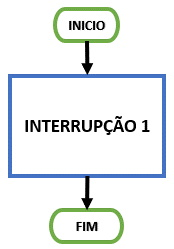
\includegraphics[scale=.85]{./image/PESTA/flowchart/Interrupt-1.jpg}
			\caption{\acs{adc} conversão}
			\label{Interrupt_1}
		\end{figure}
	\end{minipage}
	\begin{minipage}{.5\linewidth}
		\begin{figure}[H]
			\centering
			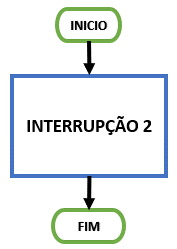
\includegraphics[scale=.85]{./image/PESTA/flowchart/Interrupt-2.jpg}
			\caption{Saltar de \textit{Menu}}
			\label{Interrupt_2}
		\end{figure}
	\end{minipage}
\end{minipage}
\minipagespace{.5}
%O código para leitura das rotinas de interrupção esta disponível nas folhas \textit{anexas} \ref{main-c}.
%É preferivel inseriri o excerto de código e descrever o funcionamento das interrupções
\begin{minipage}{.40\linewidth}
	\begin{figure}[H]
		\flushleft
		\captionsetup{justification=raggedright,singlelinecheck=false}
		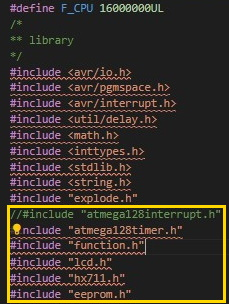
\includegraphics[scale=0.9]{./image/PESTA/Code/Livrarias.jpg}
		\caption{Bibliotecas}
		\label{Bibliotecas}
	\end{figure}
\end{minipage}
\hspace{2pt}
\begin{minipage}{.6\linewidth}
	Ao lado (\autoref{Bibliotecas}) estão as bibliotecas usadas neste projeto, as que estão dentro da caixa amarela são as que foram criadas pelo aluno.
	A filosofia usada é de criar objetos que representam o \textit{hardware} para o poder manipular via código. Como se pode observar, foi criada uma biblioteca para os temporizadores, outra para as interrupções e \ac{eeprom}, e por fim foram criadas bibliotecas para os componentes externos, isto é, o \acs{lcd} e o integrado \textbf{HX711}.\\
Uma abstração que torna simples executar qualquer algoritmo ou projeto, e isto só é possível depois de ultrapassar a barreira de desenvolver as bibliotecas.
\end{minipage}
\minipagespace{.3}
Durante este projeto foram seguidas as boas práticas de programação, como a da \texttt{indentação} específica para cada situação, e manter a estrutura de norma. Deve-se manter uma metodologia de trabalho que segue as normas, assim é percetível para qualquer programador e, não só evita bugs, mas também facilita a sua deteção. Esta é uma prática que abrange todas as linguagens.
%, por exemplo o \textbf{Python} é fundado nesse princípio.
\newpage
Quanto às interrupções é sempre um desafio, porque as tarefas têm que ser bem organizadas temporalmente para não entrar em conflitos, pretende-se assim que o código corra na função \textit{main} e as interrupções são algo esporádico e muito rápido, estas devem servir de \textit{flags} para executar rotinas na função \textit{main}, ou seja, servirem de \textit{inputs}. %%\textbf{\textcolor{green}{INPUTS}}.
%\newpage
%Passar isso para a parte de software
\emptyline
O código que executa a rotina de leitura \acs{adc} é apresentado na \autoref{HX711-read-raw}, sendo que esta é chamada pela interrupção periódica da \autoref{Interrupcao-1}, que só é ativa quando o resultado da função na \autoref{Main-While-case-1} \textbf{hx.query(\&hx)} é verdadeira.
\emptyline
{
	\lstinputlisting[language=C, caption={Interrupção 1}, captionpos=b, label=Interrupcao-1]{./input/code/Interrupcao-1.c}
}
\listingspace{.2}
{
	\lstinputlisting[language=C, caption={função de chamada \textbf{hx.query(\&hx)}}, captionpos=b, label=Main-While-case-1]{./input/code/hx_query.c}
}
\newpage
%Se apresenta código deve descreve-lo sucintamente
{
	\lstinputlisting[language=C, caption=HX711 read raw, captionpos=b, label=HX711-read-raw]{./input/code/HX711_read_raw.c}
}
Após obter um número determinado de valores discretos lidos pelo amplificador de célula de carga (HX711) é calculada uma média,
\begin{equation}
	\label{eq:Mean}
	\overline{x}  =  \frac{1}{n}\sum_{i=1}^n x_i
\end{equation}
para ser tratado e deduzido o valor correspondente do peso.
\newpage
O código da interrupção 2 está abaixo descrito na \autoref{Jump-menu} e serve para mudar de \textit{Menu} e limpar a \acs{eeprom}.
{
	\lstinputlisting[language=C, caption=Saltar de menu, captionpos=b, label=Jump-menu]{./input/code/Jump_menu.c}
}
%%%%%%%%%%%%%%%%%%%%%%%%%%%%%%%%%%%%%%%%%%%%%%%%%%%%%%%%%%

\chapter{Validação do projeto implementado}
%%%%%%%%%%%%%%%%%%%%%%%%%%%%%%%%%%%%%%%%%%%%%%%%%%%%%%%%%%
%Neste capítulo deve apresentar os testes realizados ao sistema implementado, e que devem garantir os objetivos iniciais.
Neste capítulo são apresentados os testes realizados na implementação do projeto e explicado as características de funcionamento da balança.
%%%%%%%%%%%%%%%%%%%%%%%%%%%%%%%%%%%%%%%%%%%%%%%%%%%%%%%%%%
\newpage
\section{Testagem e validação do sistema implementado}
%%%To validate is to justify why the choices made and alternatives that could be chosen.
O conhecimento adquirido ao aprofundar o funcionamento dos componentes é o ganho mais evidente na realização do projeto, que permitiu a interpretação de situações reais e deteção de anomalias (\textit{troubleshooting}).
\emptyline
Foram realizados testes, usando um osciloscópio Rigol DS1102E para afinações e resolução de anomalias e ajustando o código do anexo \ref{main-c}. O que deu mais trabalho foi a validação da biblioteca do amplificador de célula de carga HX711, que testada com os parâmetros permitidos e com diferentes frequências de transmissão. No código foram realizadas várias experiências para determinar o comportamento mais favorável. Na consulta do código que pode ser consultado nos anexos podem ver as estratégias tomadas e qual os procedimentos selecionados. Estes têm comentários com a possibilidade de alterar parâmetros que estão indicados.
%Esta justificação não é válida, tendo em conta o objetivo do trabalho !
%Apostei na marca \textbf{Atmel} devido a experiência e conhecimentos já adquiridos, se aposta-se noutra marca teria de enfrentar uma curva de aprendizagem e adaptação que no final a nível de custos beneficio seria desfavorável, pelo tempo a dispensar e de ser muito trabalhoso ao refazer tudo novamente noutra arquitetura.
\emptyline
O sensor usado é o mais comum neste tipo de aplicações pratica. Quanto ao circuito de interface a escolha foi baseada na sua precisão, ou seja, é de 24 \textit{bits} enquanto o \acs{adc} do \acs{mcu} é de apenas 10 \textit{bits} de resolução.
%Os 24 bits são necessarios? Os 10 não satifazem os objectivos ? Chega-se a este capítulo e isto não foi apresentado até agora
%%%%%%%%%%%%%%%%%%%%%%%%%%%%%%%%%%%%%%%%%%%%%%%%%%%%%%%%%%
\section{Algumas considerações acerca do funcionamento do sistema}
Quanto à funcionalidade no seu todo, a balança tem \textcolor{blue}{quatro} botões e \textcolor{blue}{três} \acsp{led}, um botão para fazer o \textit{offset} no \textcolor{green}{PORTF 0}, e dois botões com dupla função, fazer \textit{reset} para \textit{default} e incrementar, outro para entrar no menu de calibração e decrementar, o \textcolor{blue}{quarto} botão é reservado para \textit{enter} e assumir o valor introduzido na calibração.
\emptyline
O botão \textcolor{green}{PORTF 3} quando premido durante \textcolor{blue}{cinco} segundos faz um \textit{reset} para configuração \textit{default} depois de o \acs{led} no \textcolor{red}{PORTC 6} piscar \textcolor{blue}{quatro} vezes.
\emptyline
O botão \textcolor{green}{PORTF 4} quando premido durante \textcolor{blue}{cinco} segundos entra no menu de calibração do valor do \textit{gain factor} e o \acs{led} no \textcolor{red}{PORTC 7} liga. Usando os botões de incrementar e decrementar no
\textcolor{green}{PORTF 3} e \textcolor{green}{PORTF 4} pode-se alterar esse valor.
\emptyline
Para assumir o valor e sair do menu de calibração basta premir o botão colocado no \textcolor{green}{PORTF 5}. Tanto no caso de calibração como no \textit{offset} os valores são guardados na \acs{eeprom} do micro-controlador, sendo que, se retirar a alimentação do circuito este não perde os valores e o \acs{led} no \textcolor{red}{PORTC 5} permanece ligado.
\emptyline
Nos ensaios foram utilizados objetos cujo peso era conhecido, não tendo pesos de calibração disponíveis para determinar sua precisão em toda a sua gama.
%%%%%%%%%%%%%%%%%%%%%%%%%%%%%%%%%%%%%%%%%%%%%%%%%%%%%%%%%%%%%%%%
\begin{comment}
Sem contar com as despesas no equipamento para a programação do hardware que em principio só se gasta uma vez, isto é, se não se estragar. No caso do programador \textbf{Atmel-ICE} pode custar até \EUR{185.55}.
\emptyline
É de ter em conta que os preços são \textbf{PVP}, que no caso se for preços comerciais são dez vezes inferior, e se for para produção em grande escala também tem descontos por quantidade.\\
$\begin{array}{l l l}
\text{Média} & & \\
\overline{x} & = & \frac{1}{n}\sum_{i=1}^n x_i
\end{array}$
MEMS devices and structures are fabricated using conventional integrated circuit process techniques, such as lithography, deposition, and etching, together with a broad range of specially developed micromachining techniques. \cite{book-9}\\
The three essential elements in conventional silicon processing are deposition, lithography, and etching. \cite{book-9}\\
Sensitivity, Long-Term Drift and Temperature Effects (Span temperature hysteresis).
\end{comment}
%%%%%%%%%%%%%%%%%%%%%%%%%%%%%%%%%%%%%%%%%%%%%%%%%%%%%%%%%%%%%%%%

\chapter{Conclusões}
%Este parágrafo não se enquadra nas conclusões pretendidas, que se pretende que sejam relativas aos objetivos inicialmente traçados
%Uma conclusão óbvia é que a humanidade não tem esperança, demorou desde 2000 A.C até 1770 A.D, 3770 anos a descobrir de que se podia deduzir a massa dos objetos através da Lei de \textbf{Hooke}.
%Deve-se iniciar as conclusões indicando se os objetivos inicialmente propostos foram atingidos. De seguida é que devem ser apresentadas outras ideias/conclusões pertinentes, retiradas ao longo do desenvolvimento do trabalho.
O objetivo era implementar uma balança digital recorrendo aos equipamentos e componentes disponíveis no mercado. Hoje em dia com o desenvolvimento e a mudança para um mundo cada vez mais digital existem muitas lojas com estes tipos de materiais \textit{online} (ex: PTROBOTICS, Futurlec, botnroll, ALFAELEKTOR, Aquário Electrónica, ELECTROFUN, Castro Electrónica, etc ).
\emptyline
Tratando-se de uma balança digital já se sabe a priori que vai ter que se recorrer a uma célula de carga, um \acs{mcu}, amplificador de sinal e conversor \acs{adc}, e também um \textit{display}, indicadores e botões de controlo. As escolhas que foram feitas tiveram sempre em consideração o preço e o grau de complexidade do projeto, a escolha recaiu num microcontrolador de 8 \textit{bits} por se tratar de um \textit{embedded system} que trabalha diretamente com o hardware, sendo necessária uma programação numa camada de baixo nível.
\emptyline
Após obter os componentes e criar o \textit{kit} de desenvolvimento, teve de se utilizar um ambiente de trabalho e ferramentas, que são compatíveis com as escolhas feitas, neste caso o Microchip Studio, que é o representante da marca da Atmel e \acs{pic}.
\emptyline
Ao longo do relatório foram apresentados esclarecimentos e conclusões que determinaram as escolhas feitas e os procedimentos escolhidos. Além do que já foi mencionado, também se pode concluir as seguintes deduções:
\emptyline
%Não compensa desenvolver projetos que se basearam no preço de materiais \ac{pvp}, todo o lucro vai para a área comercial, se consideramos o trabalho necessário da montagem, programação, ensaios e testes para obter um produto funcional com fiabilidade e preciso respeitando as normas e diretivas, talvez se for com finalidade de produção em grande escala para entrar no mercado auferindo das regalias que ela oferece, tais como o preço da matéria prima, e mesmo assim devido a concorrência é claramente um risco se o projeto em causa é banal.
%reescrever este parágrafo, desenvolvendo melhor a ideia que pretende transmitir
\emptyline
É de salientar a importância dos equipamentos e das ferramentas utilizadas no desenvolvimento do projeto, que facilita a realização de afinações e ajustes necessários. A fiabilidade destes equipamento é fundamental para os resultados obtidos.
Outro aspeto a referir é a capacidade do aluno na consulta de \textit{datasheets} e manuais, o que é de facto um pré-requisito para o desenvolvimento do trabalho.
\emptyline
%De notar a importância dos equipamentos ou ferramentas usadas no projeto, tais como o multímetro, osciloscópio e \acsp{ide}, que nos facilita em afinações e ajustes saltando por cima de muita \textit{red tape}, dai necessário serem de confiança e fiáveis. Além do já mencionado constantemente a necessidade da habilidade de interpretar \textit{datasheets} e manuais, sendo um pré-requisito obrigatório que talvez nem é preciso o mencionar.
Deu para notar o efeito \textit{Long-term drift}, como o equipamento esteve ligado quase dois meses reparou-se que existe uma oscilação do \textit{offset}. Tal deve ser devido ao efeito de ruídos e/ou temperatura e/ou humidades. O erro é corrigido ao premir o botão de \textit{offset}.
\emptyline
Atualmente, na implementação de um projeto deste tipo, não compensa desenvolver os próprios \acs{pcb}, devido ao seu valor elevado, em comparação com o valor praticado por uma empresa dedicada a tais serviços. Outro motivo é a disponibilidade  de um vasto leque de circuitos de desenvolvimento disponíveis ao consumidor comum, prontos a ser utilizados.
\emptyline
%%%%%%%%%%%%%%%%%%%%%%%%%%%%%%%%%%%%%%%%%%%%%%%%%%%%%%%%%%
%\section{Trabalho Futuro}
Os objetivos propostos foram atingidos, no entanto é de referir alguns aspetos que podem ser reavaliados, com possibilidade de no futuro melhorar o projeto, tais como funcionar por bateria e integrar um \textit{sleep mode} de forma a desligar o \textit{display} \acs{lcd} e ficar em \textit{standby} até receber um sinal de \textit{wake up}.
\emptyline
O projeto esta disponível no \textit{\textbf{GITHUB}} \textit{link}: \url{https://github.com/BitNibble}, e possível fazer \textit{download} para quem quiser emular a experiência.
%%%%%%%%%%%%%%%%%%%%%%%%%%%%%%%%%%%%%%%%%%%%%%%%%%%%%%%%%%%%%%%%
%%\section{aspectos}
\begin{comment}
Sensitivity,Long-Term Drift e Temperature Effects (Span temperature hysteresis).
\end{comment}
%%%%%%%%%%%%%%%%%%%%%%%%%%%%%%%%%%%%%%%%%%%%%%%%%%%%%%%%%%%%%%%%
	
								% Uncomment the lines as you write the chapters,
								% where 'chapter3' refers to a file chapter3.tex
%...							% in the 'chapters' folder	
%%%%%%%%%%%%%%%%%%%%%%%BIBLIOGRAPHY%%%%%%%%%%%%%%%%%%%%%%%
% Print the bibliographic references using the ieeetr format from the 'sampleRefs.bib' file (root folder)
\printrefereces{./bibliography/Bibliography}
% Change the 'sampleRefs' name to match your .bib file name, a good option to make bib files is https://www.jabref.org/
%%%%%%%%%%%%%%%%%%%%%%%APPENDIX%%%%%%%%%%%%%%%%%%%%%%%%%%%
\appendix
% Include the appendices of the document as separate files from the 'chapters' folder
% Appendix A
%%%%%%%%%%%%%%%%%%%%%%%%%%%%%%%%%%%%%%%%%%%%%%%%%%%%%%%%%%%%%%%%
\setstretch{.9}
\chapter{Código}
\section{main}
\begin{lstlisting}[language=C, caption={main.c}, label=main-c, captionpos=b]
/*************************************************
Title: BALANCA COMERCIAL
Author: Sergio Manuel Santos
<sergio.salazar.santos@gmail.com>
File: $Id: MAIN,v 1.8.2.1 21/02/2021 Exp $
License: GNU General Public License
Software: Atmel Studio 7 (ver 7.0.129)
Hardware: Atmega128 by ETT ET-BASE
-PORTA LCD
-PORTF pin 6,7 HX711, pin 0 to 5 Buttons, 
	PIN 0 -> OFFSET, 
	PIN 3 -> DEFAULT 5sec press, and up count for div factor, 
	PIN 4 -> ENTER GAIN FACTOR MENU 5 sec press, and down count for div factor, 
	PIN 5 -> ENTER KEY to validate entered value and put in effect.
	PIN 6 and 7 -> dedicated to comunicate with Signal Amplifier
-PORTC status indicator leds
	PIN 5 -> Indicate using stored values
	PIN 6 -> Reset to default indicator (blinks four times)
	PIN 7 -> In Calibration Menu (on)
Comment:
nice
*************************************************/
#define F_CPU 16000000UL
/*
** library
*/
#include <avr/io.h>
#include <avr/pgmspace.h>
#include <avr/interrupt.h>
#include <util/delay.h>
#include <math.h>
#include <inttypes.h>
#include <stdlib.h>
#include <string.h>
#include "explode.h"
//#include "atmega128interrupt.h"
#include "atmega128timer.h"
#include "function.h"
#include "lcd.h"
#include "hx711.h"
#include "eeprom.h"
/*
** Constant and Macro
*/
#ifndef STATUS_REGISTER
	#define STATUS_REGISTER SREG
	#define GLOBAL_INTERRUPT_ENABLE 7
#endif
#define ZERO 0
#define ONE 1
#define TRUE 1
#define average_n 24 //64 -> 24
#define blink 8
#define IMASK 0x3F
#define _5sec 5
#define _10sec 10
#define minDIV 1
#define maxDIV 255
/*
** Global File variable
*/
EXPLODE F;
LCD0 lcd0;
TIMER_COUNTER0 timer0;
//INTERRUPT intx;
HX711_calibration HX711_data;
HX711_calibration* HX711_ptr;
const uint8_t sizeblock = sizeof(HX711_calibration);
HX711 hx;
float tmp;
EEPROM eprom;
char result[32];
char Menu = '1'; // Main menu selector
uint8_t counter_1 = ZERO;
uint8_t counter_2 = ZERO;
uint8_t signal = ZERO;
uint8_t count=blink;
uint16_t divfactor;
/*
** Header
*/
void PORTINIT();
/****MAIN****/
int main(void)
{
PORTINIT();
HX711_ptr = &HX711_data; // CALIBRATION DATA BUS
/***INICIALIZE OBJECTS***/
F = EXPLODEenable();
FUNC function = FUNCenable();
lcd0 = LCD0enable(&DDRA,&PINA,&PORTA);
timer0 = TIMER_COUNTER0enable(2,2); //2,2
TIMER_COUNTER1 timer1 = TIMER_COUNTER1enable(4,2); //4,2
hx = HX711enable(&DDRF, &PINF, &PORTF, 6, 7); //6,7
eprom = EEPROMenable();
//intx = INTERRUPTenable();
/******/
float value = 0;
float publish = 0;
uint8_t choice;
// Get default values to buss memory
HX711_data.offset_32 = hx.get_cal(&hx)->offset_32;
HX711_data.offset_64 = hx.get_cal(&hx)->offset_64;
HX711_data.offset_128 = hx.get_cal(&hx)->offset_128;
HX711_data.divfactor_32 = hx.get_cal(&hx)->divfactor_32;
HX711_data.divfactor_64 = hx.get_cal(&hx)->divfactor_64;
HX711_data.divfactor_128 = hx.get_cal(&hx)->divfactor_128;
HX711_data.status = hx.get_cal(&hx)->status;
/***Parameters timers***/
timer0.compoutmode(1); // troubleshooting blinking PORTB 5
/***79 and 8  -> 80 us***/
timer0.compare(60); // 8 -> 79 -> 80 us, fine tunned = 8 -> 60 -> 30.4us
timer0.start(8); // 1 -> 32 us , 8 -> 256 us , 32 64 128 256 1024
// to be used to jump menu for calibration in progress
timer1.compoutmodeA(1); // troubleshooting blinking PORTB 6
timer1.compareA(62800); // Freq = 256 -> 62800 -> 2 s
timer1.start(256);
//intx.set(1,0);
// Not necessary, if used move IDC from PORTF to PORTD with new config pinage.
// HX711 Gain
hx.set_amplify(&hx, 64); // 32 64 128
choice = hx.get_amplify(&hx);
if(choice == 1)
	divfactor = (uint16_t) HX711_data.divfactor_128;
if(choice == 2)
	divfactor = (uint16_t) HX711_data.divfactor_32;
if(choice == 3)
	divfactor = (uint16_t) HX711_data.divfactor_64;
//Get stored calibration values and put them to effect
eprom.read_block(HX711_ptr, (const void*) ZERO, sizeblock);
if(HX711_ptr->status == 1){
	//Load stored value 
	hx.get_cal(&hx)->offset_32 = HX711_ptr->offset_32;
	hx.get_cal(&hx)->offset_64 = HX711_ptr->offset_64;
	hx.get_cal(&hx)->offset_128 = HX711_ptr->offset_128;
	hx.get_cal(&hx)->divfactor_32 = HX711_ptr->divfactor_32;
	hx.get_cal(&hx)->divfactor_64 = HX711_ptr->divfactor_64;
	hx.get_cal(&hx)->divfactor_128 = HX711_ptr->divfactor_128;
	hx.get_cal(&hx)->status=ZERO;
	PORTC &= ~(ONE << 5); // troubleshooting
}
/************************************************/
//lcd0.gotoxy(1,0); // for troubleshooting
//lcd0.string_size(function.ftoa(HX711_data.status, result, ZERO), 13);
//lcd0.string_size(function.ftoa(hx.get_cal(&hx)->offset_64, result, ZERO), 13);
/************************************************/
while(TRUE){
	/******PREAMBLE******/
	lcd0.reboot(); //Reboot LCD
	F.boot(&F,PINF); //PORTF INPUT READING
	/************INPUT***********/
	if(hx.query(&hx)) 
		//Catches falling Edge instance, begins bit shifting.
		continue;
	/***geting data interval***/
	// Jump Menu signal
	if(signal == ONE){ //INPUT FROM INTERRUPT SINALS
		Menu = '2';
		signal = ZERO; // ONE SHOT
		lcd0.clear();
	}
	tmp = hx.raw_average(&hx, average_n); 
	// average_n  25 or 50, smaller means faster or more readings
	/****************************/
	switch(Menu){
		/***MENU 1***/
		case '1': // Main Program Menu
			lcd0.gotoxy(0,4); //TITLE
			lcd0.string_size("Weight Scale", 12); //TITLE
			/************************************/
			//lcd0.gotoxy(1,0); // for troubleshooting
			//lcd0.string_size(function.ftoa(hx.read_raw(&hx), result, ZERO), 13);
			/************************************/
			if((F.hl(&F) & IMASK) & ONE){ // calibrate offset by pressing button 1
			HX711_data.offset_32 = tmp;
			HX711_data.offset_64 = tmp;
			HX711_data.offset_128 = tmp;
			HX711_data.status = ONE;
			eprom.update_block(HX711_ptr, (void*) ZERO, sizeblock);
			hx.get_cal(&hx)->offset_32 = HX711_ptr->offset_32;
			hx.get_cal(&hx)->offset_64 = HX711_ptr->offset_64;
			hx.get_cal(&hx)->offset_128 = HX711_ptr->offset_128;
			hx.get_cal(&hx)->status=ZERO;
			PORTC &= ~(ONE << 5);
			}
			if(choice == 1 || choice == 11)
				value = (tmp - hx.get_cal(&hx)->offset_128) / hx.get_cal(&hx)->divfactor_128; 
				//value to be published to LCD
			if(choice == 2 || choice == 21)
				value = (tmp - hx.get_cal(&hx)->offset_32) / hx.get_cal(&hx)->divfactor_32; 
				//value to be published to LCD
			if(choice == 3 || choice == 31)
				value = (tmp - hx.get_cal(&hx)->offset_64) / hx.get_cal(&hx)->divfactor_64; 
				//value to be published to LCD
			/************************************/
			//lcd0.gotoxy(3,0); // for troubleshooting
			//lcd0.string_size(function.ftoa(tmp, result, ZERO), 13);
			//lcd0.string_size(function.ftoa(hx.get_cal(&hx)->divfactor_128, result, ZERO), 13);
			//lcd0.string_size(function.ftoa(hx.get_cal(&hx)->offset_128, result, ZERO), 13);
			/************************************/
			if (value > 1000 || value < -1000){
				publish = value / 1000;
				lcd0.gotoxy(2,1);
				lcd0.string_size(function.ftoa(publish, result, 3), 13); lcd0.string_size("Kg", 4);
			}else{
				publish = value;
				lcd0.gotoxy(2,1);
				lcd0.string_size(function.ftoa(publish, result, ZERO), 13); lcd0.string_size("gram", 4);
			}
			break;
		/***MENU 2***/
		case '2': // MANUAL CALIBRATE DIVFACTOR MENU
			/**/
			lcd0.gotoxy(0,1);
			lcd0.string_size("SETUP GAIN FACTOR",17);
			switch(choice){
				case 1: // case 128
					divfactor=hx.get_cal(&hx)->divfactor_128;
					choice=11;
					break;
				case 11: // case 128
					lcd0.gotoxy(2,9);
					if(F.hl(&F) == (ONE << 3)){
						divfactor++;
					if(divfactor > maxDIV)
						divfactor = maxDIV;
					}
					if(F.hl(&F) == (ONE << 4)){
						divfactor--;
						if(divfactor < minDIV)
							divfactor = minDIV;
					}
					HX711_data.divfactor_128 = divfactor;
					lcd0.string_size(function.ui16toa(divfactor),6);
					break;
				case 2: // case 32
					divfactor=hx.get_cal(&hx)->divfactor_32;
					choice=21;
					break;
				case 21: // case 32
					lcd0.gotoxy(2,9);
					if(F.hl(&F) == (ONE << 3)){
						divfactor++;
					if(divfactor > maxDIV)
						divfactor = maxDIV;
					}
					if(F.hl(&F) == (ONE << 4)){
						divfactor--;
						if(divfactor < minDIV)
							divfactor=minDIV;
					}
					HX711_data.divfactor_32 = divfactor;
					lcd0.string_size(function.ui16toa(divfactor),6);
					break;
				case 3: // case 64
					divfactor=hx.get_cal(&hx)->divfactor_64;
					choice=31;
					break;
				case 31: // case 64
					lcd0.gotoxy(2,9);
					if(F.hl(&F) == (ONE << 3)){
						divfactor++;
					if(divfactor > maxDIV)
						divfactor = maxDIV;
					}
					if(F.hl(&F) == (ONE << 4)){
						divfactor--;
					if(divfactor < minDIV)
						divfactor = minDIV;
					}
					HX711_data.divfactor_64 = divfactor;
					lcd0.string_size(function.ui16toa(divfactor),6);
					break;
				default:
					choice = 3;
					break;
			};
			// Exit and store value
			if((F.ll(&F) & IMASK) == (ONE << 5)){ // Button 6
				HX711_data.status = ONE;
				eprom.update_block(HX711_ptr, (void*) ZERO, sizeblock);
				hx.get_cal(&hx)->divfactor_32=divfactor;
				hx.get_cal(&hx)->divfactor_64=divfactor;
				hx.get_cal(&hx)->divfactor_128=divfactor;
				hx.get_cal(&hx)->status=ZERO;
				PORTC &= ~(ONE << 5); // troubleshooting
				PORTC |= (ONE << 7); // troubleshooting
				counter_2 = ZERO;
				Menu = '1';
				lcd0.clear();
			}
			/**/
			break;
		/****************************************/
		default:
			Menu = '1';
			break;
	};
}
}
/*
** procedure and function
*/
void PORTINIT(void)
{
	//Control buttons
	PORTF |= IMASK;
	//troubleshooting output
	DDRC = 0xFF;
	PORTC = 0xFF;
}
/*
** interrupt 1
*/
ISR(TIMER0_COMP_vect) // 15.4 us intervals
{
	/***Block other interrupts during this procedure***/
	uint8_t Sreg;
	Sreg = STATUS_REGISTER;
	STATUS_REGISTER &= ~(ONE << GLOBAL_INTERRUPT_ENABLE);
	hx.read_raw(&hx);
	/***enable interrupts again***/
	STATUS_REGISTER = Sreg;
}
/*
** interrupt 2
*/
ISR(TIMER1_COMPA_vect) // 1 second intervals
{
	/***CLEAR EEPROM OFFSET SEQUENCE START***/
	if((F.ll(&F) & IMASK) == (ONE << 3)) //button 4
	counter_1++;
	else if(counter_1 < _5sec+ONE)
	counter_1=ZERO;
	if(counter_1 > _5sec){
		counter_1 = _5sec+ONE; //lock in place
		PORTC ^= (ONE << 6); // troubleshooting
		count--;
		if(!count){ //led blinks x times
			// Delete eeprom memory ZERO
			eprom.update_block(HX711_Default, (void*) ZERO, sizeblock);
			hx.get_cal(&hx)->offset_32 = HX711_Default->offset_32;
			hx.get_cal(&hx)->offset_64 = HX711_Default->offset_64;
			hx.get_cal(&hx)->offset_128 = HX711_Default->offset_128;
			hx.get_cal(&hx)->divfactor_32 = divfactor = HX711_Default->divfactor_32;
			hx.get_cal(&hx)->divfactor_64 = divfactor = HX711_Default->divfactor_64;
			hx.get_cal(&hx)->divfactor_128 = HX711_Default->divfactor_128;
			hx.get_cal(&hx)->status = HX711_Default->status;
			PORTC |= (ONE << 5); // troubleshooting
			PORTC |= (ONE << 6); // troubleshooting
			counter_1 = ZERO;
			count=blink;
		}
	}
	/***CLEAR EEPROM OFFSET SEQUENCE END***/
	/***CAL DIVFACTOR DEFINE START***/
	if((F.ll(&F) & IMASK) == (ONE << 4)) //button 5
	counter_2++;
	else if(counter_2 < _5sec+ONE)
	counter_2=ZERO; //RESET TIMER
	if(counter_2 > _5sec){
		counter_2 = ZERO; //RESET TIMER
		signal = ONE;
		PORTC &= ~(ONE << 7); // troubleshooting
	}
	/***CAL DIVFACTOR DEFINE END***/
}
/***EOF***/
/**** Comment:
because 24 bit will have to create a vector pointer of the size of 32 bit,
then at the end do a cast to *((int32_t*)ptr).

Endurance test over 2 months, noticed drift during days, but never
getting over 20 grams. For a scale using a 50Kg cell is Excellent.
Using offset corrects the drift and precision is concise to the gram.
****/
\end{lstlisting}
%\end{verbatimtab}
%%%%%%%%%%%%%%%%%%%%%%%%%%%%%%%%%%%%%%%%%%%%%%%%%%%%%%%%%%


\section{lcd}
\begin{lstlisting}[language=C, caption={lcd.h}, label=lcd-h, captionpos=b]
/*************************************************
LCD
Author: Sergio Santos 
<sergio.salazar.santos@gmail.com>
License: GNU General Public License
Hardware: all
Date: 25102020
Comment:
tested Atemga128 16Mhz and Atmega328 8Mhz
*************************************************/
#ifndef _LCD_H_
#define _LCD_H_
/***Library***/
#include <inttypes.h>
/***Constant & Macro***/
//ASIGN PORT PINS TO LCD (can be setup in any way)
#define RS 0
#define RW 1
#define EN 2
#define NC 3
#define DB4 4
#define DB5 5
#define DB6 6
#define DB7 7
/***Global Variable***/
struct dspl{
	/******/
	void (*write)(char c, unsigned short D_I);
	char (*read)(unsigned short D_I);
	void (*BF)(void);
	void (*putch)(char c);
	char (*getch)(void);
	void (*string)(const char *s);
	void (*string_size)(const char* s, uint8_t size); // RAW
	void (*hspace)(uint8_t n);
	void (*clear)(void);
	void (*gotoxy)(unsigned int y, unsigned int x);
	void (*reboot)(void);
};
typedef struct dspl LCD0;
typedef struct dspl LCD1;
/***Header***/
LCD0 LCD0enable(volatile uint8_t *ddr, volatile uint8_t *pin, volatile uint8_t *port);
LCD1 LCD1enable(volatile uint8_t *ddr, volatile uint8_t *pin, volatile uint8_t *port);
#endif
/***Comment***
*************/
/***EOF***/
\end{lstlisting}
%\end{verbatimtab}
%%%%%%%%%%%%%%%%%%%%%%%%%%%%%%%%%%%%%%%%%%%%%%%%%%%%%%%%%%

\begin{lstlisting}[language=C, caption={lcd.c}, label=lcd-c, captionpos=b]
/*************************************************
LCD
Author: Sergio Santos 
<sergio.salazar.santos@gmail.com>
License: GNU General Public License
Hardware: all
Date: 25102020
Comment:
Tested Atemga128 16Mhz and Atmega328 8Mhz                    
*************************************************/
#ifndef F_CPU
/***Mandatory to use util/delay.h***/
#define F_CPU 16000000UL
#endif
/***Library***/
#include <avr/io.h>
#include <util/delay.h>
#include <inttypes.h>
#include "lcd.h"
/***Constant & Macro***/
#ifndef GLOBAL_INTERRUPT_ENABLE
#define GLOBAL_INTERRUPT_ENABLE 7
#endif
//CMD RS
#define INST 0
#define DATA 1
//ticks depends on CPU frequency this case 16Mhz
#define LCD_N_TICKS 3
#define LCD_BF_TICKS 10
/***Global File Variable***/
volatile uint8_t *lcd0_DDR;
volatile uint8_t *lcd0_PIN;
volatile uint8_t *lcd0_PORT;
uint8_t lcd0_detect;
volatile uint8_t *lcd1_DDR;
volatile uint8_t *lcd1_PIN;
volatile uint8_t *lcd1_PORT;
uint8_t lcd1_detect;
/***Header***/
void LCD0_inic(void);
void LCD0_write(char c, unsigned short D_I);
char LCD0_read(unsigned short D_I);
void LCD0_BF(void);
void LCD0_putch(char c);
char LCD0_getch(void);
void LCD0_string(const char* s); // RAW
void LCD0_string_size(const char* s, uint8_t size); // RAW
void LCD0_hspace(uint8_t n);
void LCD0_clear(void);
void LCD0_gotoxy(unsigned int y, unsigned int x);
void LCD0_strobe(unsigned int num);
void LCD0_reboot(void);
void LCD1_inic(void);
void LCD1_write(char c, unsigned short D_I);
char LCD1_read(unsigned short D_I);
void LCD1_BF(void);
void LCD1_putch(char c);
char LCD1_getch(void);
void LCD1_string(const char* s);
void LCD1_string_size(const char* s, uint8_t size); // RAW
void LCD1_hspace(uint8_t n);
void LCD1_clear(void);
void LCD1_gotoxy(unsigned int y, unsigned int x);
void LCD1_strobe(unsigned int num);
void LCD1_reboot(void);
unsigned int LCD_ticks(unsigned int num);
/***Procedure & Function***/
LCD0 LCD0enable(volatile uint8_t *ddr, volatile uint8_t *pin, volatile uint8_t *port)
{
	//LOCAL VARIABLES
	uint8_t tSREG;
	tSREG=SREG;
	SREG&=~(1<<GLOBAL_INTERRUPT_ENABLE);
	//ALLOCACAO MEMORIA PARA Estrutura
	LCD0 lcd0;
	//import parametros
	lcd0_DDR=ddr;
	lcd0_PIN=pin;
	lcd0_PORT=port;
	//inic variables
	*lcd0_DDR=0x00;
	*lcd0_PORT=0xFF;
	lcd0_detect=*lcd0_PIN & (1<<NC);
	//Direccionar apontadores para PROTOTIPOS
	lcd0.write=LCD0_write;
	lcd0.read=LCD0_read;
	lcd0.BF=LCD0_BF;
	lcd0.putch=LCD0_putch;
	lcd0.getch=LCD0_getch;
	lcd0.string=LCD0_string;
	lcd0.string_size=LCD0_string_size; // RAW
	lcd0.hspace=LCD0_hspace;
	lcd0.clear=LCD0_clear;
	lcd0.gotoxy=LCD0_gotoxy;
	lcd0.reboot=LCD0_reboot;
	//LCD INIC
	LCD0_inic();
	SREG=tSREG;
	//
	return lcd0;
}
void LCD0_inic(void)
{
	//LCD INIC
	*lcd0_DDR=(1<<RS)|(1<<RW)|(1<<EN)|(0<<NC);
	*lcd0_PORT=(1<<NC);
	/***INICIALIZACAO LCD**datasheet*/
	_delay_ms(40);
	LCD0_write(0x33,INST); //function set
	_delay_us(39);
	LCD0_write(0x33,INST); //function set
	_delay_us(39);
	LCD0_write(0x2B,INST); //function set
	_delay_us(37);
	LCD0_write(0x0C,INST);// display on/off control
	_delay_us(37);
	LCD0_write(0x01,INST);// clear display
	_delay_ms(1.53);
	LCD0_write(0x06,INST);// entry mode set (crazy settings)
	_delay_us(37);
	/***INICIALIZATION END***/
	//LCD0_write(0x1F,INST);// cursor or display shift
	//_delay_us(39);
	//LCD0_write(0x03,INST);// return home
	//_delay_ms(1.53);
}
void LCD0_write(char c, unsigned short D_I)
{
	*lcd0_PORT&=~(1<<RW);//lcd as input WRITE INSTRUCTION
	if(D_I) *lcd0_PORT|=(1<<RS); else *lcd0_PORT&=~(1<<RS);
	*lcd0_DDR|=(1<<DB4)|(1<<DB5)|(1<<DB6)|(1<<DB7);//mcu as output
	*lcd0_PORT|=(1<<EN);
	if(c & 0x80) *lcd0_PORT|=1<<DB7; else *lcd0_PORT&=~(1<<DB7);
	if(c & 0x40) *lcd0_PORT|=1<<DB6; else *lcd0_PORT&=~(1<<DB6);
	if(c & 0x20) *lcd0_PORT|=1<<DB5; else *lcd0_PORT&=~(1<<DB5);
	if(c & 0x10) *lcd0_PORT|=1<<DB4; else *lcd0_PORT&=~(1<<DB4);
	*lcd0_PORT&=~(1<<EN);
	LCD_ticks(LCD_N_TICKS);
	*lcd0_PORT|=(1<<EN);
	if(c & 0x08) *lcd0_PORT|=1<<DB7; else *lcd0_PORT&=~(1<<DB7);
	if(c & 0x04) *lcd0_PORT|=1<<DB6; else *lcd0_PORT&=~(1<<DB6);
	if(c & 0x02) *lcd0_PORT|=1<<DB5; else *lcd0_PORT&=~(1<<DB5);
	if(c & 0x01) *lcd0_PORT|=1<<DB4; else *lcd0_PORT&=~(1<<DB4);
	*lcd0_PORT&=~(1<<EN);
	LCD_ticks(LCD_N_TICKS);
}
char LCD0_read(unsigned short D_I)
{
	char c=0x00;
	*lcd0_DDR&=~((1<<DB4)|(1<<DB5)|(1<<DB6)|(1<<DB7));//mcu as input
	*lcd0_PORT|=(1<<DB4)|(1<<DB5)|(1<<DB6)|(1<<DB7);//pullup resistors
	*lcd0_PORT|=(1<<RW);//lcd as output READ INSTRUCTION
	if(D_I) *lcd0_PORT|=(1<<RS); else *lcd0_PORT&=~(1<<RS);
	*lcd0_PORT|=(1<<EN);
	if(*lcd0_PIN & (1<<DB7)) c|=1<<7; else c&=~(1<<7);
	if(*lcd0_PIN & (1<<DB6)) c|=1<<6; else c&=~(1<<6);
	if(*lcd0_PIN & (1<<DB5)) c|=1<<5; else c&=~(1<<5);
	if(*lcd0_PIN & (1<<DB4)) c|=1<<4; else c&=~(1<<4);
	*lcd0_PORT&=~(1<<EN);
	LCD_ticks(LCD_N_TICKS);
	*lcd0_PORT|=(1<<EN);
	if(*lcd0_PIN & (1<<DB7)) c|=1<<3; else c&=~(1<<3);
	if(*lcd0_PIN & (1<<DB6)) c|=1<<2; else c&=~(1<<2);
	if(*lcd0_PIN & (1<<DB5)) c|=1<<1; else c&=~(1<<1);
	if(*lcd0_PIN & (1<<DB4)) c|=1<<0; else c&=~(1<<0);
	*lcd0_PORT&=~(1<<EN);
	LCD_ticks(LCD_N_TICKS);
	return c;
}
void LCD0_BF(void)
{
	unsigned int i;
	char inst=0x80;
	for(i=0;0x80&inst;i++){
		inst=LCD0_read(INST);
		LCD_ticks(LCD_BF_TICKS);
		if(i>10)// if something goes wrong
		break;
	}
}
void LCD0_putch(char c)
{
	LCD0_write(c,DATA);
	LCD0_BF();
}
char LCD0_getch(void)
{
	char c;
	c=LCD0_read(DATA);
	LCD0_BF();
	return c;
}
void LCD0_string(const char* s)
{
	char tmp;
	while(*s){
		tmp=*(s++);
		LCD0_write(tmp,DATA);
		LCD0_BF();
	}
}
void LCD0_string_size(const char* s, uint8_t size)
{
	char tmp;
	uint8_t pos=0;
	while(*s){
		tmp=*(s++);
		pos++;
		if(pos>size) // 1 TO SIZE+1
		break;
		LCD0_write(tmp,DATA);
		LCD0_BF();
	}
	while(pos<size){ // TO SIZE
		pos++;
		LCD0_write(' ',DATA);
		LCD0_BF();
	}
}
void LCD0_hspace(uint8_t n)
{
	for(;n;n--){
		LCD0_write(' ',DATA);
		LCD0_BF();
	}
}
void LCD0_clear(void)
{
	LCD0_write(0x01,INST);
	_delay_ms(1.53);
}
void LCD0_gotoxy(unsigned int y, unsigned int x)
{
	switch(y){
		case 0:
		LCD0_write((0x80+x),INST);
		LCD0_BF();
		break;
		case 1:
		LCD0_write((0xC0+x),INST);
		LCD0_BF();
		break;
		case 2:
		LCD0_write((0x94+x),INST);//0x94
		LCD0_BF();
		break;
		case 3:
		LCD0_write((0xD4+x),INST);//0xD4
		LCD0_BF();
		break;
		default:
		break;
	}
}
void LCD0_strobe(unsigned int num)
{
	*lcd0_PORT|=(1<<EN);
	LCD_ticks(num);
	*lcd0_PORT&=~(1<<EN);
}
void LCD0_reboot(void)
{
	uint8_t tSREG;
	tSREG=SREG;
	SREG&=~(1<<GLOBAL_INTERRUPT_ENABLE);
	//low high detect pin NC
	uint8_t i;
	uint8_t tmp;
	tmp=*lcd0_PIN & (1<<NC);
	i=tmp^lcd0_detect;
	i&=tmp;
	if(i)
	LCD0_inic();
	lcd0_detect=tmp;
	SREG=tSREG;
}
/************************************************/
LCD1 LCD1enable(volatile uint8_t *ddr, volatile uint8_t *pin, volatile uint8_t *port)
{
	//LOCAL VARIABLES
	uint8_t tSREG;
	tSREG=SREG;
	SREG&=~(1<<GLOBAL_INTERRUPT_ENABLE);
	//ALLOCACAO MEMORIA PARA Estrutura
	LCD1 lcd1;
	//import parametros
	lcd1_DDR=ddr;
	lcd1_PIN=pin;
	lcd1_PORT=port;
	//inic variables
	*lcd1_DDR=0x00;
	*lcd1_PORT=0xFF;
	lcd1_detect=*lcd1_PIN & (1<<NC);
	//Direccionar apontadores para PROTOTIPOS
	lcd1.write=LCD1_write;
	lcd1.read=LCD1_read;
	lcd1.BF=LCD1_BF;
	lcd1.putch=LCD1_putch;
	lcd1.getch=LCD1_getch;
	lcd1.string=LCD1_string;
	lcd1.string_size=LCD1_string_size; // RAW
	lcd1.hspace=LCD1_hspace;
	lcd1.clear=LCD1_clear;
	lcd1.gotoxy=LCD1_gotoxy;
	lcd1.reboot=LCD1_reboot;
	//LCD INIC
	LCD1_inic();
	SREG=tSREG;
	//
	return lcd1;
}
void LCD1_inic(void)
{
	//LCD INIC
	*lcd1_DDR=(1<<RS)|(1<<RW)|(1<<EN)|(0<<NC);
	*lcd1_PORT=(1<<NC);
	/***INICIALIZACAO**LCD**datasheet***/
	_delay_ms(40);
	LCD1_write(0x33,INST); //function set
	_delay_us(39);
	LCD1_write(0x33,INST); //function set
	_delay_us(39);
	LCD1_write(0x2B,INST); //function set
	_delay_us(37);
	LCD1_write(0x0C,INST);// display on/off control
	_delay_us(37);
	LCD1_write(0x01,INST);// clear display
	_delay_ms(1.53);
	LCD1_write(0x06,INST);// entry mode set (crazy settings)
	_delay_us(37);
	/***INICIALIZATION END***/
	//LCD1_write(0x1F,INST);// cursor or display shift
	//_delay_us(39);
	//LCD1_write(0x03,INST);// return home
	//_delay_ms(1.53);
}
void LCD1_write(char c, unsigned short D_I)
{
	*lcd1_PORT&=~(1<<RW);//lcd as input WRITE INSTRUCTION
	if(D_I) *lcd1_PORT|=(1<<RS); else *lcd1_PORT&=~(1<<D_I);
	*lcd1_DDR|=(1<<DB4)|(1<<DB5)|(1<<DB6)|(1<<DB7);//mcu as output
	*lcd1_PORT|=(1<<EN);
	if(c & 0x80) *lcd1_PORT|=1<<DB7; else *lcd1_PORT&=~(1<<DB7);
	if(c & 0x40) *lcd1_PORT|=1<<DB6; else *lcd1_PORT&=~(1<<DB6);
	if(c & 0x20) *lcd1_PORT|=1<<DB5; else *lcd1_PORT&=~(1<<DB5);
	if(c & 0x10) *lcd1_PORT|=1<<DB4; else *lcd1_PORT&=~(1<<DB4);
	*lcd1_PORT&=~(1<<EN);
	LCD_ticks(LCD_N_TICKS);
	*lcd1_PORT|=(1<<EN);
	if(c & 0x08) *lcd1_PORT|=1<<DB7; else *lcd1_PORT&=~(1<<DB7);
	if(c & 0x04) *lcd1_PORT|=1<<DB6; else *lcd1_PORT&=~(1<<DB6);
	if(c & 0x02) *lcd1_PORT|=1<<DB5; else *lcd1_PORT&=~(1<<DB5);
	if(c & 0x01) *lcd1_PORT|=1<<DB4; else *lcd1_PORT&=~(1<<DB4);
	*lcd1_PORT&=~(1<<EN);
	LCD_ticks(LCD_N_TICKS);
}
char LCD1_read(unsigned short D_I)
{
	char c=0x00;
	*lcd1_DDR&=~((1<<DB4)|(1<<DB5)|(1<<DB6)|(1<<DB7));//mcu as input
	*lcd1_PORT|=(1<<DB4)|(1<<DB5)|(1<<DB6)|(1<<DB7);//pullup resistors
	*lcd1_PORT|=(1<<RW);//lcd as output READ INSTRUCTION
	if(D_I) *lcd1_PORT|=(1<<RS); else *lcd1_PORT&=~(1<<D_I);
	*lcd1_PORT|=(1<<EN);
	if(*lcd1_PIN & (1<<DB7)) c|=1<<7; else c&=~(1<<7);
	if(*lcd1_PIN & (1<<DB6)) c|=1<<6; else c&=~(1<<6);
	if(*lcd1_PIN & (1<<DB5)) c|=1<<5; else c&=~(1<<5);
	if(*lcd1_PIN & (1<<DB4)) c|=1<<4; else c&=~(1<<4);
	*lcd1_PORT&=~(1<<EN);
	LCD_ticks(LCD_N_TICKS);
	*lcd1_PORT|=(1<<EN);
	if(*lcd1_PIN & (1<<DB7)) c|=1<<3; else c&=~(1<<3);
	if(*lcd1_PIN & (1<<DB6)) c|=1<<2; else c&=~(1<<2);
	if(*lcd1_PIN & (1<<DB5)) c|=1<<1; else c&=~(1<<1);
	if(*lcd1_PIN & (1<<DB4)) c|=1<<0; else c&=~(1<<0);
	*lcd1_PORT&=~(1<<EN);
	LCD_ticks(LCD_N_TICKS);
	return c;
}
void LCD1_BF(void)
{
	unsigned int i;
	char inst=0x80;
	for(i=0;0x80&inst;i++){
		inst=LCD1_read(INST);
		LCD_ticks(LCD_BF_TICKS);
		if(i>10)// if something goes wrong
		break;
	}
}
void LCD1_putch(char c)
{
	LCD1_write(c,DATA);
	LCD1_BF();
}
char LCD1_getch(void)
{
	char c;
	c=LCD1_read(DATA);
	LCD1_BF();
	return c;
}
void LCD1_string(const char* s)
{
	char tmp;
	while(*s){
		tmp=*(s++);
		LCD1_write(tmp,DATA);
		LCD1_BF();
	}
}
void LCD1_string_size(const char* s, uint8_t size)
{
	char tmp;
	uint8_t pos=0;
	while(*s){
		tmp=*(s++);
		pos++;
		if(pos>size)
		break;
		LCD1_write(tmp,DATA);
		LCD1_BF();
	}
	while(pos<size){
		pos++;
		LCD1_write(' ',DATA);
		LCD1_BF();
	}
}
void LCD1_hspace(uint8_t n)
{
	for(;n;n--){
		LCD1_write(' ',DATA);
		LCD1_BF();
	}
}
void LCD1_clear(void)
{
	LCD1_write(0x01,INST);
	_delay_ms(1.53);
}
void LCD1_gotoxy(unsigned int y, unsigned int x)
{
	switch(y){
		case 0:
		LCD1_write((0x80+x),INST);
		LCD1_BF();
		break;
		case 1:
		LCD1_write((0xC0+x),INST);
		LCD1_BF();
		break;
		case 2:
		LCD1_write((0x94+x),INST);//0x94
		LCD1_BF();
		break;
		case 3:
		LCD1_write((0xD4+x),INST);//0xD4
		LCD1_BF();
		break;
		default:
		break;
	}
}
void LCD1_strobe(unsigned int num)
{
	*lcd1_PORT|=(1<<EN);
	LCD_ticks(num);
	*lcd1_PORT&=~(1<<EN);
}
void LCD1_reboot(void)
{
	//LOCAL VARIABLES
	uint8_t tSREG;
	tSREG=SREG;
	SREG&=~(1<<GLOBAL_INTERRUPT_ENABLE);
	//low high detect pin NC
	uint8_t i;
	uint8_t tmp;
	tmp=*lcd1_PIN & (1<<NC);
	i=tmp^lcd1_detect;
	i&=tmp;
	if(i)
	LCD1_inic();
	lcd1_detect=tmp;
	SREG=tSREG;
}
unsigned int LCD_ticks(unsigned int num)
{
	unsigned int count;
	for(count=0;count<num;count++)
	;
	return count;
}
/***Interrupt***/
/***Comment***
*************/
/***EOF***/
\end{lstlisting}
%\end{verbatimtab}
%%%%%%%%%%%%%%%%%%%%%%%%%%%%%%%%%%%%%%%%%%%%%%%%%%%%%%%%%%

\section{hx711}
\begin{lstlisting}[language=C, caption={hx711.h}, label=hx711-h, captionpos=b]
/*************************************************
HX711
Author: Sergio Santos
<sergio.salazar.santos@gmail.com>
License: GNU General Public License
Hardware: Atmega 128
Date: 08032021_start
Comment:

*************************************************/
#ifndef _HX711_H_
#define _HX711_H_
/***Library***/
#include <avr/io.h>
#include <inttypes.h>
/***Constant & Macro***/

/***Global Variable***/
//calibration
typedef struct{
	int32_t offset_32; // ZERO set point A
	int32_t offset_64; // ZERO set point B 64
	int32_t offset_128; // ZERO set point B 128
	uint8_t divfactor_32; // interval A
	uint8_t divfactor_64; // interval B
	uint8_t divfactor_128; // interval B
	uint8_t status;
}HX711_calibration;
HX711_calibration* HX711_Default;
//device
struct hx711{
	volatile uint8_t readflag; // indicate start of bit shifting
	uint8_t trigger; // pickup signal
	uint8_t amplify; // number of end clock cycles
	uint8_t ampcount; // count down final amplify pulses
	uint8_t bitcount; // count down 24 bit
	uint8_t buffer[4]; // reading buffer
	uint8_t bufferindex; // buffer index
	int32_t raw_reading; // reading to be published
	int32_t sum;
	uint8_t av_n;
	float raw_mean;
	HX711_calibration cal_data;
	/******/
	uint8_t (*get_amplify)(struct hx711* self);
	uint8_t (*read_bit)(void);
	void (*set_amplify)(struct hx711* self, uint8_t amplify);
	uint8_t (*query)(struct hx711* self);
	int32_t (*read_raw)(struct hx711* self);
	float (*raw_average)(struct hx711* self, uint8_t n);
	uint8_t (*get_readflag)(struct hx711* self);
	HX711_calibration* (*get_cal)(struct hx711* self);
};
typedef struct hx711 HX711;
/***Header***/
HX711 HX711enable(volatile uint8_t *ddr, volatile uint8_t *pin,
volatile uint8_t *port, uint8_t datapin, uint8_t clkpin);
#endif
/***/
/***Comment***
*************/
/***EOF***/
\end{lstlisting}
%\end{verbatimtab}
%%%%%%%%%%%%%%%%%%%%%%%%%%%%%%%%%%%%%%%%%%%%%%%%%%%%%%%%%%

\begin{lstlisting}[language=C, caption={hx711.c}, label=hx711-c, captionpos=b]
/*************************************************
HX711
Author: Sergio Santos
<sergio.salazar.santos@gmail.com>
License: GNU General Public License     
Hardware: Atmega 128
Date: 08032021_start
Comment:
Nice
*************************************************/
#ifndef F_CPU
/***Mandatory to use util/delay.h***/
#define F_CPU 16000000UL
#endif
/***Library***/
#include <avr/io.h>
#include <inttypes.h>
#include "hx711.h"
/***Constant & Macro***/
#ifndef STATUS_REGISTER
#define STATUS_REGISTER SREG
#define GLOBAL_INTERRUPT_ENABLE 7
#endif
#define ZERO 0
#define OFF 0
#define ONE 1
#define ON 0xFF
#define HX711_ticks 36 // fine tunned to 36
#define HX711_ADC_bits 24
#define HX711_VECT_SIZE 4
/***Global File Variable***/
/***/
HX711_calibration HX711_Default_50Kg = {
	.offset_32 = 35900,
	.offset_64 = 72200,
	.offset_128 = 143600,
	.divfactor_32 = 23,
	.divfactor_64 = 46,
	.divfactor_128 = 92,
	.status = ZERO
};
/***/
volatile uint8_t *hx711_DDR;
volatile uint8_t *hx711_PIN;
volatile uint8_t *hx711_PORT;
uint8_t hx711_datapin;
uint8_t hx711_clkpin;
int32_t* ptr;
/***Header***/
uint8_t HX711_get_amplify(HX711* self);
void HX711_reset_readflag(HX711* self);
uint8_t HX711_read_bit(void);
void HX711_set_amplify(HX711* self, uint8_t amplify);
uint8_t HX711_query(HX711* self);
int32_t HX711_read_raw(HX711* self);
float HX711_raw_average(HX711* self, uint8_t n);
uint8_t HX711_get_readflag(HX711* self);
HX711_calibration* HX711_get_cal(HX711* self);
/***Procedure & Function***/
HX711 HX711enable(volatile uint8_t *ddr, volatile uint8_t *pin, volatile uint8_t *port, 
uint8_t datapin, uint8_t clkpin)
{
	//LOCAL VARIABLES
	uint8_t tSREG;
	tSREG = STATUS_REGISTER;
	STATUS_REGISTER &= ~(1<<GLOBAL_INTERRUPT_ENABLE);
	//ALLOCACAO MEMORIA PARA Estrutura
	HX711 hx711;
	//import parametros
	hx711_DDR = ddr;
	hx711_PIN = pin;
	hx711_PORT = port;
	hx711_datapin = datapin;
	hx711_clkpin = clkpin;
	//inic variables
	*hx711_DDR |= (ONE<<clkpin);
	*hx711_PORT |= (ONE<<datapin);
	hx711.readflag = ZERO;
	hx711.trigger = ZERO;
	hx711.amplify = ONE;
	hx711.ampcount = ONE;
	hx711.bitcount = HX711_ADC_bits;
	hx711.buffer[0] = ZERO;
	hx711.buffer[1] = ZERO;
	hx711.buffer[2] = ZERO;
	hx711.buffer[3] = ZERO;
	hx711.bufferindex = HX711_VECT_SIZE-ONE;
	hx711.raw_reading = ZERO;
	hx711.sum = ZERO;
	hx711.av_n = ZERO;
	hx711.raw_mean = ZERO;
	// offset para mesa usada.
	hx711.cal_data.offset_32 = HX711_Default_50Kg.offset_32; // to subtract B
	hx711.cal_data.offset_64 = HX711_Default_50Kg.offset_64; // to subtract A 64
	hx711.cal_data.offset_128 = HX711_Default_50Kg.offset_128; // to subtract A 128
	//GAIN FACTOR
	hx711.cal_data.divfactor_32 = HX711_Default_50Kg.divfactor_32; // to divide
	hx711.cal_data.divfactor_64 = HX711_Default_50Kg.divfactor_64; // to divide
	hx711.cal_data.divfactor_128 = HX711_Default_50Kg.divfactor_128; // to divide
	hx711.cal_data.status = HX711_Default_50Kg.status;
	HX711_Default = &HX711_Default_50Kg;
	//Direccionar apontadores para PROTOTIPOS
	hx711.get_amplify=HX711_get_amplify;
	hx711.read_bit=HX711_read_bit;
	hx711.set_amplify=HX711_set_amplify;
	hx711.query=HX711_query;
	hx711.read_raw=HX711_read_raw;
	hx711.raw_average=HX711_raw_average;
	hx711.get_readflag=HX711_get_readflag;
	hx711.get_cal=HX711_get_cal;
	STATUS_REGISTER = tSREG;
	// returns a copy
	return hx711;
}
uint8_t HX711_get_amplify(HX711* self)
{
	return self->amplify;
}
void HX711_reset_readflag(HX711* self)
{
	self->readflag=OFF;
}
uint8_t HX711_read_bit(void)
{	
	uint16_t ibool;
	*hx711_PORT|=(ONE<<hx711_clkpin);
	/**0.1us minimum**/
	for(ibool=ZERO; ibool<HX711_ticks; ibool++); //inline delay
	ibool=*hx711_PIN & (ONE<<hx711_datapin);
	*hx711_PORT &= ~(ONE<<hx711_clkpin);
	return ibool;
}
// Gain selector
// AVDD connected to 5V, channel B gain=32
void HX711_set_amplify(HX711* self, uint8_t amplify)
{
	switch(amplify){
		case 128:
		self->amplify = ONE; //channel A
		self->ampcount = ONE;
		break;
		case 32:
		self->amplify = 2; //channel B
		self->ampcount = 2; 
		break;
		case 64:
		self->amplify = 3; //channel A
		self->ampcount = 3;
		break;
		default:
		self->amplify = ONE;
		self->ampcount = ONE;
		break;
	}
}
uint8_t HX711_query(HX711* self)
{
	uint8_t flag=OFF; // one shot
	if(!self->readflag){
		if(!(*hx711_PIN & (ONE << hx711_datapin))){
			self->readflag=ON;
			flag=ON;
		}
	}
	return flag;
}
/***
Function to be used in the interrupt routine with appropriate cycle period.
***/
int32_t HX711_read_raw(HX711* self)
{
	uint8_t aindex, bindex;
	int32_t value;
	aindex = self->bufferindex-ONE;
	bindex = self->bitcount-ONE;
	ptr=(int32_t*)self->buffer;
	/***Interrupt 24 times sequence plus gain pulses***/
	if(self->readflag){
		if(self->bitcount){
			if (HX711_read_bit())
			self->buffer[aindex] |= ONE<<(bindex-(aindex*8));
			self->bitcount--;
			if(self->bitcount == 16)
			self->bufferindex=2;
			if(self->bitcount == 8)
			self->bufferindex=ONE;
		}else{
			if(self->ampcount){
				HX711_read_bit();
				self->ampcount--;
			}else{
				value = *(ptr);
				self->raw_reading = value;
				self->bitcount = HX711_ADC_bits;
				self->bufferindex = HX711_VECT_SIZE-ONE;
				self->ampcount = self->amplify;
				self->buffer[0] = ZERO;
				self->buffer[1] = ZERO;
				self->buffer[2] = ZERO;
				self->buffer[3] = ZERO;
				self->trigger = ONE;
				/***Reset ready for next query***/
				HX711_reset_readflag(self);
			}
		}
	}
	return self->raw_reading;
}
float HX711_raw_average(HX711* self, uint8_t n)
{
	if(self->trigger){
		if(self->av_n < n){
			self->sum += self->raw_reading;
			self->av_n++;
		}else{
			self->av_n = ZERO;
			self->raw_mean = self->sum / n;
			self->sum = ZERO;
			self->sum += self->raw_reading;
			self->av_n++;
		}
		self->trigger = ZERO;
	}
	return self->raw_mean;
}
uint8_t HX711_get_readflag(HX711* self)
{
	return self->readflag;
}
HX711_calibration* HX711_get_cal(HX711* self)
{
	return &(self->cal_data);
}
/***Interrupt***/
/***comment***
Have to use vector to store 32 bit size word, then do a cast (int32_t*)
to retrieve the value.
*************/
/***EOF***/
\end{lstlisting}
%\end{verbatimtab}
%%%%%%%%%%%%%%%%%%%%%%%%%%%%%%%%%%%%%%%%%%%%%%%%%%%%%%%%%%

\chapter{Definições}
%%%%%%%%%%%%%%%%%%%%%%%%%%%%%%%%%%%%%%%%%%%%%%%%%%%%%%%%%%%%%%%%%%%%%%%%%%%%%
\begin{minipage}[t]{0.50\linewidth}
	\begin{definition}
		Capacit\^{a}ncia
		\begin{flalign*}
			Q_c(t) =& \int^t i(t) \quad dt & \\
			=& Q_c(0^-)+\int_{0^-}^t i(t) \quad dt & \\
			V_c(t) =& \frac{Q_c(t)}{C} & \\
			=& \frac{1}{C} \quad \int^t i_c(t) \quad dt & \\
			=& \frac{Q_c(0^-)}{C} + \frac{1}{C} \quad \int_0^t i_c(t) \quad dt & \\
			=& V(0^-) + \frac{1}{C} \quad \int_0^t i_c(t) \quad dt & \\
			i_c(t) =& C \quad \dfrac{d V_c(t)}{dt} &
		\end{flalign*}\par
	\end{definition}
\end{minipage}
%
\begin{minipage}[t]{0.50\linewidth}
	\begin{definition}
		Indut\^{a}ncia
		\begin{flalign*}
			\psi_L(t) =& \int^t V_L(t) \quad dt & \\
			=& \psi_L(0^-)+\int_{0^-}^t V_L(t) \quad dt & \\
			V_L(t) =& L \quad \dfrac{d i_L(t)}{dt} & \\
			i_L(t) =& \frac{\psi_L(t)}{L} & \\
			=& \frac{1}{L} \quad \int^t V_L(t) \quad dt & \\
			=& \frac{\psi_L(0^-)}{L} + \frac{1}{L} \quad \int_0^t V_L(t) \quad dt &  \\
			=& i_L(0^-) + \frac{1}{L} \quad \int_0^t V_L(t) \quad dt &
		\end{flalign*}\par
	\end{definition}
\end{minipage}
\\
\\
\\
\\
\par
\begin{minipage}[t]{0.5\linewidth}
	\begin{definition}
		Resist\^{e}ncia
		\begin{flalign*}
			V_R(t) =& R \quad i_R(t) & \\
			i_R(t) =& \frac{V_R(t)}{R} &
		\end{flalign*}\par
	\end{definition}
\end{minipage}
%
\begin{minipage}[t]{0.5\linewidth}
	\begin{definition}
		Valor M\'{e}dio
		\begin{flalign*}
			X_{av} =& \frac{1}{T} \; \int_0^T X(t) dt &
		\end{flalign*}\par
	\end{definition}
	%
	\begin{definition}
		Valor Eficaz
		\begin{flalign*}
			X_{ef} =& \sqrt{ \frac{1}{T} \; \int_0^T \overset{\text{2}}{X(t)} dt } &
		\end{flalign*}\par
	\end{definition}
\end{minipage}
%%%%%%%%%%%%%%%%%%%%%%%%%%%%%%%%%%%%%%%%%%%%%%%%%%%%%%%%%%%%%%%%%%%%%%%%%%%%%

\label{anexo-definition-1}
\chapter{Física}
%%%%%%%%%%%%%%%%%%%%%%%%%%%%%%%%%%%%%%%%%%%%%%%%%%%%%%%%%%%%%%%%
\fbox{
	\begin{minipage}{.6\textwidth}
		\section*{Motion}
		{\Large $  x_{(t)}=x_{o}\,+\,v_{o}\,t\,+\,\frac{1}{2}\,a\,t^2  $}
		\emptyline
		{\Large $  x_{(t)} \quad \xtofrom[\int \,dt]{\od{}{t}} \quad v_{(t)} \quad \xtofrom[\int \,dt]{\od{}{t}} \quad a_{(t)} $}
	\end{minipage}
}
\emptyline
\fbox{
\begin{minipage}[c]{.45\textwidth}
	\section*{Força  [N] [Kgf]}
	\large
	$\begin{array}{ l l l l l }
		\sum F_{(t)} & = & M \; a_{(t)} & = & M \; \ddot{x}_{(t)}
	\end{array}$
	\newline
	\newline
	$\begin{array}{ l l l }
		\sum F_{R} & = & \sum F_{action} \; - \; \sum F_{reaction}
	\end{array}$
	\newline
	\newline
	$\begin{array}{ l l l }
		f_{(t)} & = & -K \; x_{(t)} \\
		f_{(t)} & = & -B \; \dot{x}_{(t)}
	\end{array}$
	\newline
	\newline
	\newline
	%%%There are only forces if there is a physical object subject to them.
\end{minipage}
}
%\newline
\hspace{.1cm}
%\newline
\fbox{
\begin{minipage}[c]{.45\textwidth}
	\section*{Torque [N.m]}
	\large
	$\begin{array}{ l l l l l }
		\sum T_{(t)} & = & J \; \gamma_{(t)} & = & M \; \ddot{\theta}_{(t)}
	\end{array}$
	\newline
	\newline
	$\begin{array}{ l l l }
		\sum T_{R} & = & \sum T_{action} \; - \; \sum T_{reaction}
	\end{array}$
	\newline
	\newline
	$\begin{array}{ l l l }
		T_{(t)} & = & -K \; \theta_{(t)} \\
		T_{(t)} & = & -B \; \dot{\theta}_{(t)} \\
		T & = & F \times r
	\end{array}$
	\newline
	\newline
	%%%Never mix potatoes with bananas.
\end{minipage}
}
\newline
\vspace{.6cm}
\newline
\begin{minipage}[c]{.5\textwidth}
	\section*{Energia [Joule]}
	\vspace{.1cm}
	\Large
	$\begin{array}{ l l l }
		W & = & F \; d \\
		W & = & P \; \Delta t \\
		E & = & M \; C^{2}
	\end{array}$
\end{minipage}
\begin{minipage}[c]{.5\textwidth}
	\begin{figure}[H]
		\flushleft
		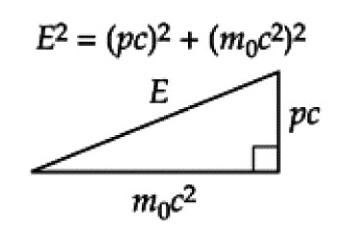
\includegraphics[scale=0.6]{./image/General/Einstein.jpg}
		\caption*{\cite{book-2}}
		\label{Einstein}
	\end{figure}
\end{minipage}
\newline
\vspace{.6cm}
\newline
\begin{minipage}[!b]{.5\textwidth}
	\section*{Energia Cinética [Joule]}
	\Large
	$\begin{array}{ l l l }
		E_{c} & = & \frac{1}{2} \; m \; v^{2}
	\end{array}$
\end{minipage}
\begin{minipage}[!b]{.5\textwidth}
	\section*{Energia Potencial [Joule]}
	\Large
	$\begin{array}{ l l l }
		E_{p} & = & \; m \; g \; h
	\end{array}$
\end{minipage}
\newline
\vspace{.6cm}
\newline
\begin{minipage}[l]{\textwidth}
	\section*{Energia Térmica}
	\Large
	$\begin{array}{ l l l l }
		Q - Heat \quad energy & & & \\
		Q_{(t)} - temperature & & & \\
		R - heat \quad resistance & & & \\
		& Q & = & \frac{Q_{1(t)} - Q_{2(t)}}{R}
	\end{array}$
\end{minipage}
%%%%%%%%%%%%%%%%%%%%%%%%%%%%%%%%%%%%%%%%%%%%%%%%%%%%%%%%%%%%%%%%
%%%%%%%%%%%%%%%%%%%%%%%%%%%%%%%%%%%%%%%%%%%%%%%%%%%%%%%%%%%%%%%%
%%%%%%%%%%%%%%%%%%%%%%%%%%%%%%%%%%%%%%%%%%%%%%%%%%%%%%%%%%%%%%%%
\begin{comment}
\newline
\vspace{1cm}
\newline
$\frac{A \times B}{C}\times D \approx E$,
\newline
\begin{minipage}{0pt}
	$$\begin{array}{l | l}
		\text{Média aritmetica dados classificados} & \text{Variância de uma amostra dados classificados} \\
		\overline{x} = \frac{1}{n}\sum_{i=1}^cx_in_i = \sum_{i=1}^cx_if_i & s^2 = \frac{1}{n-1}\sum_{i=1}^c (x_i-\bar{x})^2 n_i
	\end{array}$$
\end{minipage}
\newline
\vspace{1cm}
\newline
$IC_{1-\alpha}=\left[ A, B\right]$ ; para $1-\alpha = 0.95$, $\alpha=0.05$, $\frac{\alpha}{2}=0.025$
\newline
\vspace{1cm}
\newline
Zona critica $Z_c=Z_{1-\frac{\alpha}{2}}=\Phi^{-1}(0.975) \cong 1.96$
\newline
\vspace{1cm}
\newline
$P\left( A \leqslant \mu \leqslant B \right) = 1-\alpha$ \\
$\triangle=Z_c\times\frac{\delta}{\sqrt{n}}$ \\
$A = \bar{x}-\triangle \qquad and \qquad B = \bar{x}+\triangle$ \\
$\therefore$\\
$IC_{A_{0.95}}=\left[ \; 18.8877 \: , \: 21.1956 \; \right]$ \hspace{1cm} and \hspace{1cm} $IC_{B_{0.95}}=\left[ \; 20.4519 \: , \: 22.6314 \; \right]$
\newline
\vspace{1cm}
\newline
$\left[ \; \mu \; \right]$
\newline
\vspace{1cm}
\newline
$\bar{y}_{A_0}$ = 6,6111 \qquad $\bar{y}_{B_0}$ = 7,5111 \qquad $n=90$ \\
$\delta_A$ = 2,3112 \qquad $\delta_B$ = 2,5140
\newline
\vspace{1cm}
\newline
$P(Y_A < 6)=P(Y_A \leqslant 5)=F_{i_B}(5) \cong 0,3677 $  \quad e \quad $P(Y_B < 6)=P(Y_B \leqslant 5)=F_{i_B}(5) \cong 0,2444$ \\
\newline
\vspace{1cm}
\newline
$\hat{P_A}-\hat{P_B} \sim N \left( p_A - p_B ; \frac{p_A\:q_A}{n_A} + \frac{p_B\:q_B}{n_B}\right)$ \hspace{1cm}
$\triangle=z_{(1-\frac{\alpha}{2})} \;\sqrt{\frac{\hat{p_A} \: \hat{q_A}}{n_A}+\frac{\hat{p_B} \: \hat{q_B}}{n_B}}$ \hspace{1cm} $q=(1-p)$
\newline
\vspace{1cm}
\newline
$IC_{97\%}(\hat{P_A}-\hat{P_B})=\left[(\hat{p_A}-\hat{p_B})-\triangle \: ; \: (\hat{p_A}-\hat{p_B})+\triangle \right]$
\newline
\vspace{1cm}
\newline
$\hat{P_A}-\hat{P_B} \sim N \left( 0,1233 \; ; \; 0,02788\right)$ \hspace{1cm}
$z_{(1-\frac{\alpha}{2})}=\phi^{-1}(0,985)=2,1701$
\newline
\vspace{1cm}
\newline
Recorrendo a calculadora casio $fx-9860GII$ :
\newline
\vspace{1cm}
\newline
$\triangle= InvNorm(0.985)\sqrt{\frac{0.3677(1-0.3677)}{90}+\frac{0.2444(1-0.2444)}{90}}\: \cong \:0.3677$
\\
$\therefore$
\\
$IC_{97\%}(\hat{P_A}-\hat{P_B})=\left[ \; (\hat{p_A}-\hat{p_B}) \:-\: 0,3624 \: ; \: (\hat{p_A}-\hat{p_B}) \:+\: 0,3624 \; \right]$
\newline
\vspace{1cm}
\newline
\begin{minipage}[l]{0pt}
	$$\left\lbrace\begin{array}{l}
		H_0: \quad \mu_A-\mu_B=0 \\
		\\
		H_1: \quad \mu_A-\mu_B<0
	\end{array}\right.$$
\end{minipage}
\newline
\vspace{1cm}
\newline
\begin{minipage}[l]{0pt}
	$$\left\lbrace\begin{array}{c}
		\mu \;=\; 0 \\
		\delta \;=\; s \\
	\end{array}\right.$$
\end{minipage}
\hspace{3cm} $\Longrightarrow$ \hspace{1cm}
\begin{minipage}[l]{0pt}
	\[\bar{X}=\bar{X}_A-\bar{X}_B \quad \backsim N \left( 0\:,\: \frac{\delta_A^2}{n_A}+\frac{\delta_B^2}{n_B} \right) \quad ; \quad \frac{\delta_A^2}{n_A}+\frac{\delta_B^2}{n_B}\;\cong0.6558 \]
\end{minipage}
\newline
\vspace{1cm}
\newline
$P(\bar{X}_{H_0} \leqslant C)=0.05 \quad \implies \quad RC_X\left] -\infty \:,\: -1.332 \right] \qquad \bar{x}_A-\bar{x}_B=-1.5 \in RC_X $
\newline
\vspace{1cm}
\newline
\begin{minipage}[l]{0pt}
	\[  z_0\:=\: \frac{\bar{x}_A-\bar{x}_B}{\sqrt{\frac{\delta_A^2}{n_A}+\frac{\delta_B^2}{n_B}}}\:\cong\: -1.8523 \qquad
	RC_z \:=\: \left] -\infty \:,\: -1.6448 \right]  \qquad
	pvalue \:=\: P(Z<z_0) \:=\: 0.032 \]
\end{minipage}
\newline
\vspace{1cm}
\newline
\hspace*{5cm} \underline{Condição NEE:}\\
\begin{minipage}[l]{0pt}
	$$\left\lbrace\begin{array}{c}
		\mu \;=\; 0 \\
		\delta \;=\; s \\
	\end{array}\right.$$
\end{minipage}
\hspace{3cm} $\Longrightarrow$ \hspace{1cm}
\begin{minipage}[l]{0pt}
	\[ \bar{Y}=\bar{Y_A}-\bar{Y_B} \quad \backsim N \left( 0\:,\: \frac{\delta_A^2}{n_A}+\frac{\delta_B^2}{n_B} \right) \quad ; \quad \frac{\delta_A^2}{n_A}+\frac{\delta_B^2}{n_B} \; \cong 0.1296 \]
\end{minipage}
\newline
\vspace{1cm}
\newline
$P(\bar{Y}_{H_0} \leqslant C)=0.05 \quad \implies \quad RC_Y\left] -\infty \:,\: -0.5921 \right] \qquad \bar{y}_A-\bar{y}_B=-0.9 \in RC_Y $
\newline
\vspace{1cm}
\newline
\begin{minipage}[l]{0pt}
	\[  z_0\:=\: \frac{\bar{y}_A-\bar{y}_B}{\sqrt{\frac{\delta_A^2}{n_A}+\frac{\delta_B^2}{n_B}}}\:\cong\: -2.5 \qquad
	RC_z \:=\: \left] -\infty \:,\: -1.6448 \right]  \qquad
	pvalue \:=\: P(Z<z_0) \:=\: 0.0062 \]
\end{minipage}
\newline
\vspace{1cm}
\newline
\begin{minipage}[l]{0pt}
	$$\left\lbrace\begin{array}{l}
		H_0: X \backsim N (20.0417\;,\;6.4494^2) \\
		\\
		H_1: X \nsim N (20.0417\;,\;6.4494^2)
	\end{array}\right.$$
\end{minipage}
\newline
\vspace{1cm}
\newline
\hspace*{5cm} \underline{NEE Região B:} \\
\begin{minipage}[l]{0pt}
	$$\left\lbrace\begin{array}{l}
		H_0: X \backsim N (7.5111\;,\;2.5140^2) \\
		\\
		H_1: X \nsim N (7.5111\;,\;2.5140^2)
	\end{array}\right.$$
\end{minipage}
\newline
\vspace{1cm}
\newline
$q_0=\sum_{i=1}^n \frac{(n_i-e_i)^2}{e_i} \;\backsim\; \chi_{(k-m-1)}^2$
\newline
\vspace{1cm}
\newline
$RC_{\chi^2}=\left[ \: InvChiCD(0.05,5) \:,\: +\infty \; \right] \quad \rightarrow \quad RC_{\chi_2}=\left[ \: 11.0705 \:,\: +\infty \; \right]$
\newline
\vspace{1cm}
\newline
$q_0=8.5532$ < 11.0705
\newline
\vspace{1cm}
\newline
$\left[ \; \mu \; \right]$
\newline
\vspace{1cm}
\newline
$\bar{y}_{A_0}$ = 6,6111 \qquad $\bar{y}_{B_0}$ = 7,5111 \qquad $n=90$ \\
$\delta_A$ = 2,3112 \qquad $\delta_B$ = 2,5140
\newline
\vspace{1cm}
\newline
$P(Y_A < 6)=P(Y_A \leqslant 5)=F_{i_B}(5) \cong 0,3677 $  \quad e \quad $P(Y_B < 6)=P(Y_B \leqslant 5)=F_{i_B}(5) \cong 0,2444$
\newline
\vspace{1cm}
\newline
$\hat{P_A}-\hat{P_B} \sim N \left( p_A - p_B ; \frac{p_A\:q_A}{n_A} + \frac{p_B\:q_B}{n_B}\right)$ \hspace{1cm}
$\triangle=z_{(1-\frac{\alpha}{2})} \;\sqrt{\frac{\hat{p_A} \: \hat{q_A}}{n_A}+\frac{\hat{p_B} \: \hat{q_B}}{n_B}}$ \hspace{1cm} $q=(1-p)$
\newline
\vspace{1cm}
\newline
$IC_{97\%}(\hat{P_A}-\hat{P_B})=\left[(\hat{p_A}-\hat{p_B})-\triangle \: ; \: (\hat{p_A}-\hat{p_B})+\triangle \right]$
\newline
\vspace{1cm}
\newline
$\hat{P_A}-\hat{P_B} \sim N \left( 0,1233 \; ; \; 0,02788\right)$ \hspace{1cm}
$z_{(1-\frac{\alpha}{2})}=\phi^{-1}(0,985)=2,1701$
\newline
\vspace{1cm}
\newline
Recorrendo a calculadaora casio $fx-9860GII$ :
\newline
\vspace{1cm}
\newline
$\triangle= InvNorm(0.985)\sqrt{\frac{0.3677(1-0.3677)}{90}+\frac{0.2444(1-0.2444)}{90}}\: \cong \:0.3677$
\\
$\therefore$
\\
$IC_{97\%}(\hat{P_A}-\hat{P_B})=\left[ \; (\hat{p_A}-\hat{p_B}) \:-\: 0,3624 \: ; \: (\hat{p_A}-\hat{p_B}) \:+\: 0,3624 \; \right]$
\newline
\vspace{1cm}
\newline
\begin{minipage}[l]{0pt}
	$$\left\lbrace\begin{array}{l}
		H_0: \quad \mu_A-\mu_B=0 \\
		\\
		H_1: \quad \mu_A-\mu_B<0
	\end{array}\right.$$
\end{minipage}
\newline
\vspace{1cm}
\newline
\begin{minipage}[l]{0pt}
	$$\left\lbrace\begin{array}{c}
		\mu \;=\; 0 \\
		\delta \;=\; s \\
	\end{array}\right.$$
\end{minipage}
\hspace{3cm} $\Longrightarrow$ \hspace{1cm}
\begin{minipage}[l]{0pt}
	\[\bar{X}=\bar{X}_A-\bar{X}_B \quad \backsim N \left( 0\:,\: \frac{\delta_A^2}{n_A}+\frac{\delta_B^2}{n_B} \right) \quad ; \quad \frac{\delta_A^2}{n_A}+\frac{\delta_B^2}{n_B}\;\cong0.6558 \]
\end{minipage}
\newline
\vspace{1cm}
\newline
$P(\bar{X}_{H_0} \leqslant C)=0.05 \quad \implies \quad RC_X\left] -\infty \:,\: -1.332 \right] \qquad \bar{x}_A-\bar{x}_B=-1.5 \in RC_X $
\newline
\vspace{1cm}
\newline
\begin{minipage}[l]{0pt}
	\[  z_0\:=\: \frac{\bar{x}_A-\bar{x}_B}{\sqrt{\frac{\delta_A^2}{n_A}+\frac{\delta_B^2}{n_B}}}\:\cong\: -1.8523 \qquad
	RC_z \:=\: \left] -\infty \:,\: -1.6448 \right]  \qquad
	pvalue \:=\: P(Z<z_0) \:=\: 0.032 \]
\end{minipage}
\newline
\vspace{1cm}
\newline
\hspace*{5cm} \underline{Condição NEE:}\\
\begin{minipage}[l]{0pt}
	$$\left\lbrace\begin{array}{c}
		\mu \;=\; 0 \\
		\delta \;=\; s \\
	\end{array}\right.$$
\end{minipage}
\hspace{3cm} $\Longrightarrow$ \hspace{1cm}
\begin{minipage}[l]{0pt}
	\[ \bar{Y}=\bar{Y_A}-\bar{Y_B} \quad \backsim N \left( 0\:,\: \frac{\delta_A^2}{n_A}+\frac{\delta_B^2}{n_B} \right) \quad ; \quad \frac{\delta_A^2}{n_A}+\frac{\delta_B^2}{n_B} \; \cong 0.1296 \]
\end{minipage}
\newline
\vspace{1cm}
\newline
$P(\bar{Y}_{H_0} \leqslant C)=0.05 \quad \implies \quad RC_Y\left] -\infty \:,\: -0.5921 \right] \qquad \bar{y}_A-\bar{y}_B=-0.9 \in RC_Y $
\newline
\vspace{1cm}
\newline
\begin{minipage}[l]{0pt}
	\[  z_0\:=\: \frac{\bar{y}_A-\bar{y}_B}{\sqrt{\frac{\delta_A^2}{n_A}+\frac{\delta_B^2}{n_B}}}\:\cong\: -2.5 \qquad
	RC_z \:=\: \left] -\infty \:,\: -1.6448 \right]  \qquad
	pvalue \:=\: P(Z<z_0) \:=\: 0.0062 \]
\end{minipage}
\newline
\vspace{1cm}
\newline
\begin{minipage}[l]{0pt}
	$$\left\lbrace\begin{array}{l}
		H_0: X \backsim N (20.0417\;,\;6.4494^2) \\
		\\
		H_1: X \nsim N (20.0417\;,\;6.4494^2)
	\end{array}\right.$$
\end{minipage}
\newline
\vspace{1cm}
\newline
\hspace*{5cm} \underline{NEE Região B:} \\
\begin{minipage}[l]{0pt}
	$$\left\lbrace\begin{array}{l}
		H_0: X \backsim N (7.5111\;,\;2.5140^2) \\
		\\
		H_1: X \nsim N (7.5111\;,\;2.5140^2)
	\end{array}\right.$$
\end{minipage}
\newline
\vspace{1cm}
\newline
$q_0=\sum_{i=1}^n \frac{(n_i-e_i)^2}{e_i} \;\backsim\; \chi_{(k-m-1)}^2$
\newline
\vspace{1cm}
\newline
$RC_{\chi^2}=\left[ \: InvChiCD(0.05,5) \:,\: +\infty \; \right] \quad \rightarrow \quad RC_{\chi_2}=\left[ \: 11.0705 \:,\: +\infty \; \right]$
\newline
\vspace{1cm}
\newline
$q_0=8.5532$ < 11.0705
\newline
\vspace{1cm}
\newline
\begin{minipage}[l]{0pt}
	$$\left\lbrace\begin{array}{l}
		H_0: \bar{X}_{H_0} \backsim N (0 \;,\; 0.6558) \\
		\\
		H_1: \bar{X}_{H_1} \backsim N (-1.5 \;,\; 0.6558)
	\end{array}\right.$$
\end{minipage}
\newline
\vspace{1cm}
\newline
$\beta=P(Aceitar H_0 | H_0 é Falsa)$ \\
$\beta=(\bar{X}_{H_1} \:>\: -1.332)$	\\
$\beta=NormCD(-1.332,99999999,\sqrt{0.6558},-1.5)=0.4178$ \\
Potência do teste \\
$1-\beta=P(Rejeitar H_0 | H_0 é Falsa)=0.5822$
\newline
\vspace{1cm}
\newline
NEE Região B:\\
\begin{minipage}[l]{0pt}
	$$\left\lbrace\begin{array}{l}
		H_0: \bar{Y}_{H_0} \backsim N (0 \;,\; 0.1296) \\
		\\
		H_1: \bar{Y}_{H_1} \backsim N (-0.9 \;,\; 0.1296)
	\end{array}\right.$$
\end{minipage}
\newline
\vspace{1cm}
\newline
$\beta=P(Aceitar H_0 | H_0 é Falsa)$ \\
$\beta=(\bar{Y}_{H_1} \:>\: -0.5921)$	\\
$\beta=NormCD(-0.5921,99999999,\sqrt{0.1296},-0.9)=0.1962$ \\
Potência do teste \\
$1-\beta=P(Rejeitar H_0 | H_0 é Falsa)=0.8038$
\newline
\vspace{1cm}
\newline
$\chi^2$
\end{comment}
%%%%%%%%%%%%%%%%%%%%%%%%%%%%%%%%%%%%%%%%%%%%%%%%%%%%%%%%%%%%%%%%

\label{anexo-physics-1}
%%%%%%%%%%%%%%%%%%%%%%%%%%%%%%%%%%%%%%%%%%%%%%%%%%%%%%%%%%%%%%%%

	% Uncomment the lines as you write the appendices,
%\include{chapters/appendixB}	% or comment the lines if not used
%%%%%%%%%%%%%%%%%%%%%%GLOSSARY%%%%%%%%%%%%%%%%%%%%%%%%%%%%
\newpage
\footnote{Apontamento}
%%%%%%%%%%%%%%%%%%%%%%%%%%%%%%%%%%%%%%%%%%%%%%%%%%%%%%%%%%
\end{document}
%%%%%END%%%%%END%%%%%END%%%%%END%%%%%END%%%%%%%%%%%%%%%%%%
%%%%%%%%%%%%%%%%%%%%%%COMMENTS%%%%%%%%%%%%%%%%%%%%%%%%%%%%
%%%%%%%%%%%%%%%%%%%%%%%%%%%%%%%%%%%%%%%%%%%%%%%%%%%%%%%%%%